\documentclass[12pt]{article}
\usepackage{geometry}
\geometry{left=1in,right=0.75in,top=1in,bottom=1in}
\newcommand{\Problem}{E}
\newcommand{\Team}{2523245}
\usepackage{newtxtext}
\usepackage{amsmath,amssymb,amsthm}
\usepackage{newtxmath} % must come after amsXXX
\usepackage[pdftex]{graphicx}
\usepackage{xcolor}
\usepackage{fancyhdr}
\usepackage{booktabs}
\usepackage{changepage}
\usepackage{enumitem}
\usepackage{subcaption}
\usepackage{makecell}
\usepackage{multirow}
\usepackage{algorithm}
\usepackage{caption}
\usepackage{pdfpages}
\usepackage{algpseudocode}
\captionsetup{skip=0.05cm}
\lhead{Team \Team}
\rhead{}
\cfoot{}
\newtheorem{theorem}{Theorem}
\newtheorem{corollary}[theorem]{Corollary}
\newtheorem{lemma}[theorem]{Lemma}
\newtheorem{definition}{Definition}
\begin{document}
\graphicspath{{.}}  % Place your graphic files in the same directory as your main document
\DeclareGraphicsExtensions{.pdf, .jpg, .tif, .png}
\thispagestyle{empty}
\vspace*{-16ex}
\centerline{\begin{tabular}{*3{c}}
	\parbox[t]{0.3\linewidth}{\begin{center}\textbf{Problem Chosen}\\ \Large \textcolor{red}{\Problem}\end{center}}
	& \parbox[t]{0.3\linewidth}{\begin{center}\textbf{2025\\ ICM\\ Summary Sheet}\end{center}}
	& \parbox[t]{0.3\linewidth}{\begin{center}\textbf{Team Control Number}\\ \Large \textcolor{red}{\Team}\end{center}}	\\
	\hline
\end{tabular}}
%%%%%%%%%%%%%%% 环境配置结束 %%%%%%%%
%%%%%%%%%%% Summary开始 %%%%%%%%%%%
\setcounter{page}{1}
\begin{center}
\Large{\textbf{Stop the Expands, Preserve the Lands!}}
\vspace{0.2cm}


\large{\textbf{Summary}}
\vspace{-0.4cm}
\end{center}

Agricultural ecosystems are complicated. In this paper, we integrate diverse methodologies to quantify and visualize the evolution pace of agricultural ecosystems at different stages.


For task 1, Elementary Ecology Interaction Model (\textbf{EEIM}) and its corresponding destroyer model (\textbf{EEDM}) are proposed to constitute the basic food web model, respectively representing \textbf{natural evolution processes excluding human factors} and \textbf{human-induced disturbances to ecosystems}. Firstly, we assume an ideal elementary food web. Based on \textbf{Food Web Dynamics}, we modified \textbf{Lotka-Volterra} basic model to describe relationships of species in our agricultural ecosystem without any intervention. Then, we take agricultural cycle and season into consideration and obtain the comprehensive biomass. Using \textbf{Shannon Index}, we calculate species richness. 
EEDM is built on a \textbf{Multi-layer Perceptron} which reaches an accuracy of \textbf{91.3\%} on validation datasets. It calculates how humans' overuse of chemicals deteriorates biodiversity and ecosystem stability. EEDM reveals that \textbf{the loss of species richness} triggered by chemicals is likely to \textbf{reach its peak value 27.66\% in year 2027} then shrinks at an extremely slow ratio.

For task 2, firstly, we propose a \textbf{Generalized Pascal's Triangle }which successfully portraits \textbf{the dynamic process} on the reemergence of native species and \textbf{visualizes its deeper mechanisms}. Then we introduce \textbf{Resilience Stability and Resistance Stability Models} to quantify the effects of native species' reemerging behavior and explain its \textbf{inner ecological mechanisms} from another perspective.

For task 3, we firstly determine the effects of herbicide removal using the food web model and conclude that: \textbf{Chemicals' removal is merely a short-term solution} to stabilize agricultural ecosystems, which \textbf{may trigger an unstable system due to soaring weeds} and other competitors against native crops. The \textbf{long-term solution is to introduce bats and other higher-level predators} (e.g., grass snakes). Then we employ the \textbf{convolution model} to visualize and quantify bats' interaction with other creatures, namely the \textbf{Bats Kernels}. We further discover that \textbf{a higher biodiversity does not necessarily contributes to a stable ecosystem}. Ratherly, only when species richness falls within the scope of \textbf{[22\%,75\%]} can it truly stabilizes. By integrating Broadened Pascal's Triangle, convolution models and Resistance Stability Model, we comprehensively evaluate bats' influence on overall ecosystem stability. \textbf{Grass Snake} is chosen as the comparison creature, where we discover that although both snakes and bats contribute to stability from a macro perspective, \textbf{their deeper mechanisms differ significantly}. As a higher-level consumer, grass snake keeps the stability by \textbf{preying on lower-level predators}. Contrarily, bats, as lower-level consumers, contribute to stability directly by \textbf{controlling pest population}.  

For task 4, we integrate initiatives associated with organic farming, establish a \textbf{multi-objective programming model}, and utilize the \textbf{simulated annealing algorithm} to determine the optimal implementation effects of organic farming methods. We also focus on exploring the impacts of organic farming across multiple dimensions, progressively analyzing how these initiatives achieve the best outcomes.

Finally, the \textbf{Monte Carlo Algorithm} is applied to verify the robustness of our model, acquiring a mean loss of \textbf{0.03123} and standard deviation loss  of \textbf{0.00917}, demonstrating the robust feature of  models. 


\textbf{Keywords: }Lotka-Volterra Model; Multi-layer Perceptron; Generalized Pascal's Triangle; Resistance Stability; Convolution Kernel; Multi-objective Programming; Simulated Annealing Algorithms.





%%%%%%%%%%% Summary结束 %%%%%%%%%%%
%%%%%%%%%%%% 生成目录 %%%%%%%%%%%%
\clearpage
\pagestyle{fancy}
\tableofcontents 
\newpage
\rhead{Page \thepage\ }
%%%%%%%%%%% 生成目录结束 %%%%%%%%%%%%%
%%%%%%%%%% 正文开始 %%%%%%%%%%%%%%
\section{Introduction}
\subsection{Problem Background}
\hspace{1.5em}\textit{``Where is our home?''asked the honeybee.``It's lost, forever.''}--an excerpt from the \textit{Aseop's Fables}.

Humans are top consumers in food webs. Although the prosperity of contemporary industries has witnessed a flourished human society, it also beholds our relentless pursuit of gain. Like a ceaseless dance with shadows, every step forward casts a deeper shadow upon the soul, and yet the thirst for more never finds its quenching.  Pests invade, lands deteriorate$\dots$ The once thriving forests shift into farmlands, but humans seem to be never satisfied. We turn to chemicals, trying to make up for the damages we've caused. Pesticides, herbicides, fertilizers$\dots$. Making rooms for agriculture in itself is not a matter of reproach, the key is, how we perceive it. Stability, biodiversity, species richness, few of them are considered before a land is exploited, but now, it's time. A comprehensive food web model could get us through the darkness, a complete assessment system lifts us to a brighter future. It's our mission, it's the world's mission.
\begin{figure}[h]
	\centering
	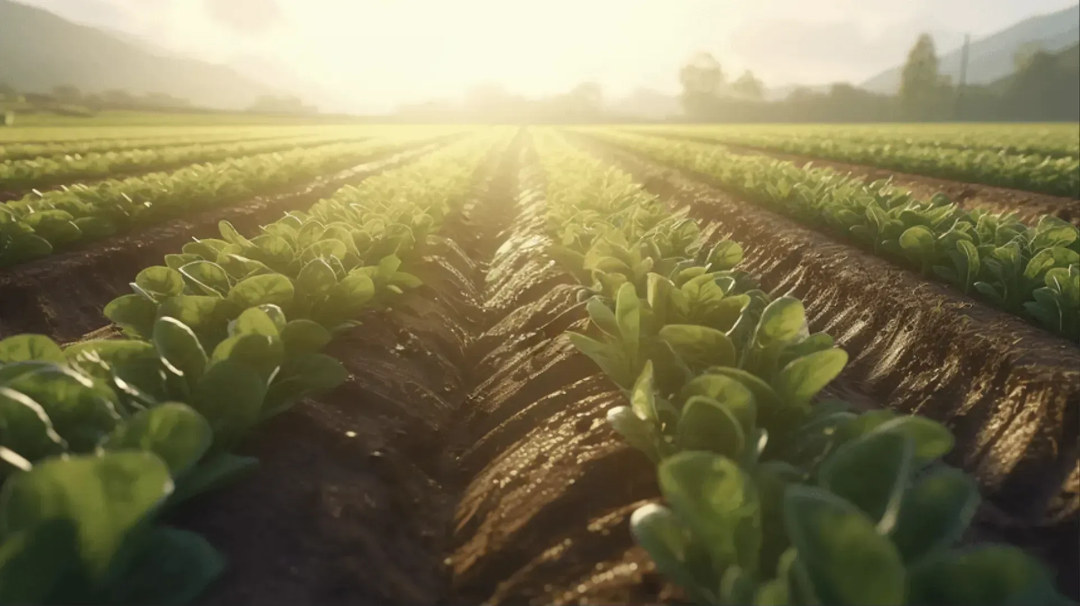
\includegraphics[width=0.4\textwidth,trim=0cm 5cm 0cm 0.2cm, clip]{./figures/intro.png}
	\caption{Forest-to-farm agricultural ecosystem}
\end{figure}
\subsection{Restatement of the Problems}
\hspace{1.5em}The primary goal of modelling process is to track habitat change from forest-to-farm where diverse indicators ought to be considered. Firstly, establish a food web model considering both natural and human factors, including food chain components, seasonal characteristics, chemical usages, etc. Their corresponding impacts on the ecosystem stability is required to be analyzed.
Secondly, analyze the influence of native species' reemergence and their interactions with environments,  using two species as the case study.
Thirdly, consider the impacts on ecosystem stability when herbicide is removed. Describe how introduced bats interact with environments and identify a similar species.
Finally, analyze the multiple implications of organic agriculture and evaluate different scenarios incorporating varying components of organic farming.

\subsection{Overview of Our Works}
\hspace{1.5em}To avoid over-complicated descriptions, we intuitively present our work in flowcharts, as is illustrated in figure \ref{dianluban}.
\begin{figure}[h]
    \centering
    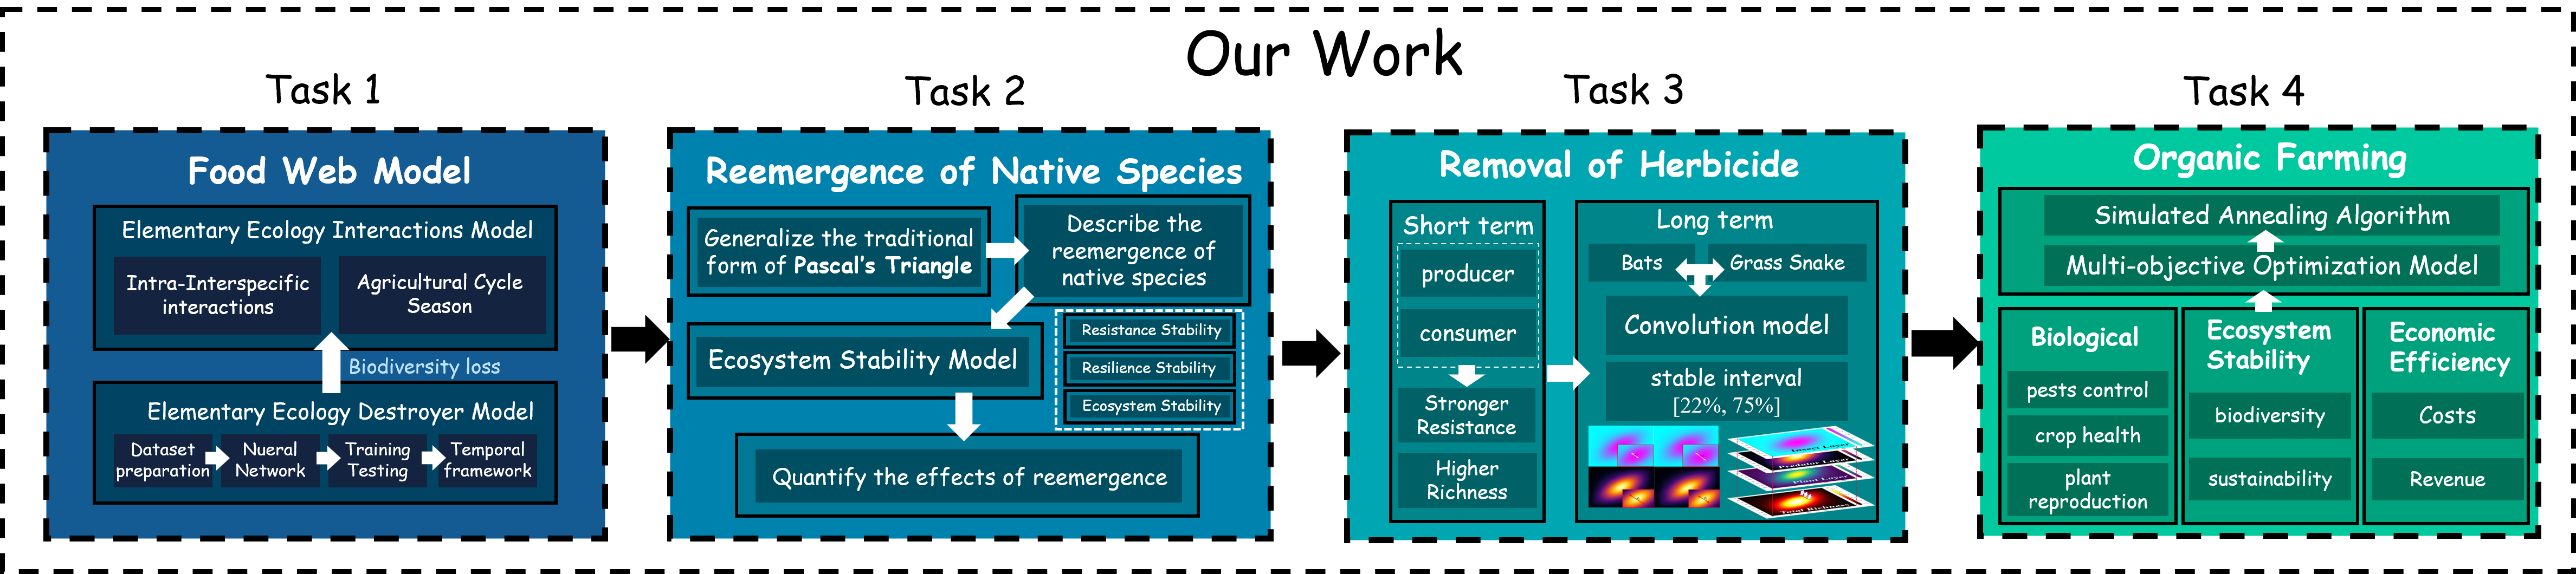
\includegraphics[width=\textwidth]{./figures/dianluban.png}
    \caption{Overview of our work.}
    \label{dianluban}
\end{figure}

\section{Assumptions and Justification}
\hspace{1.5em}\textbf{Assumption 1: }Total biomass and species quantity of living creatures in agricultural ecosystems follow a distribution strictly based on a certain proportion during specified periods.

\textbf{Justification 1: }Biomass and species richness are generally  influenced by factors including resource availability, human interventions and other climate-related elements, all of which operate within a predictable temporal and spatial framework. They constrain the evolution process of ecosystems, leading to a forseeable species distribution and biomass accumulation during specific periods. 

\textbf{Assumption 2: }In the primary stage of agricultural ecosystem evolution, biodiversity and species richness are positively proportional to ecosystem stability.

\textbf{Justification 2: }Existing researches \cite{1} \cite{2} \cite{3} have revealed that either low or high phylogenetic diversity enhances stability directly.

\textbf{Assumption 3: }The agricultural ecosystem under study is relatively stable, with no major natural disasters or human-induced disturbances during the research period. The ecosystem is influenced solely by its internal dynamics, agricultural cycles, and human activities.

\textbf{Justification 3: }Ecosystems are highly complex systems influenced by multiple factors. By excluding extreme external disturbances and analyzing the primary factors, the analytical process could be simplified, while also enhancing the generalization of our conclusions.



\section{Notations}
\hspace{1.5em}Key variables of the paper are listed in table \ref{notations}. Specific sub-variables which merely occur in corresponding sections are defined at the beginning of each chapter.  
\begin{table}[h]
    \centering
    \setlength{\tabcolsep}{45pt}
    \begin{tabular}{cc}
    \toprule[2pt]
    \textbf{Notations} & \textbf{Explanations (units)} \\
    \midrule[1pt]
        $LSR$ & Loss of Species Richness (\%).\\
        $RTS^{*}$ & Resistance Stability of ecosystems (/).\\
         $RLS^{*}$ & Resilience Stability of ecosystems (/).\\
         $TES^{*}$ & Total Ecosystem Stability (/). \\
         $B_i$ & Biomass of Species $i$ \ ($kg/m^2$) \\
         $K_i$ & Maximum Carrying Capacity for Species $i$ (/)\\
         $a_{i-j}$ & Efficiency of species $i$ preying on species $j$ (/)\\
         $\beta_{i-j}$ & Efficiency of species $j$ captured by species $i$ (/)\\
    \bottomrule[2pt]
    \end{tabular}
    \caption{Key notations of the paper, where * represents that the variable is a dimensionless quantity which qualitatively describe the extent of corresponding subjects.}
    \label{notations}
\end{table}


\section{Establishment of the Food Web Model}
\hspace{1.5em}Food webs are sophisticated. Before humans get involved, a majority of ecosystems evolve in their exclusive dynamics. Noticing such natural characteristic, we separate the food web into two sub-models. 

Firstly, We propose the Elementary Ecology Interaction Model (EEIM) to simulate natural processes of ecosystem evolution excluding human factors (e.g., chemical pollution). Then we design the Elementary Ecology Destroyer Model (EEDM) to introduce human interference into ecosystem evolution. Finally, the Food Web Model is established by integrating EEIM and EEDM, which comprehensively interprets the evolution dynamics of forest-to-farm agricultural ecosystems.
\subsection{Elementary Ecology Interaction Model, EEIM}
\subsubsection{Food Web Dynamics}
\hspace{1.5em}Food web dynamics serves to describe trends of interactions among species and the energy flow in ecosystems. Absorbing energies from the circumstances, producers pass them to consumers. Then via the metabolism of consumers and decomposers, the energies return to external surroundings. Considering that the forest is newly converted to agricultural use, biomass of the chief species (e.g., crops, insects and birds) is bound to change. Therefore, we introduce the Food Web Dynamics. Let a community nourishes $n$ species, the dynamics of such region can be described by multiple differential equations:
\begin{equation}
    \frac{dB_i}{dt}=f_i(B)\hspace{1em}(i=1,2,...,n)
    \label{Bi}
\end{equation}

\subsubsection{Intra-Interspecific Interactions Among Species}
\hspace{1.5em}We primarily focus on intraspecific interactions and feeding relationship in the area, of which intraspecific interactions depend solely on the environment and biomass of population itself, while the feeding relationship is additionally influenced by the species that it interacts with. The latter can be referred to as Consumer-Resource(C-R) interactions[7].Therefore, equation \eqref{Bi} can be optimized into:
\begin{equation}
    \frac{dB_i}{dt}=f_i(B_i)+\sum_{j=1,j\neq i}^n f_{ij}(B_i,B_j)-\sum_{k=1,k\neq i}^n f_{ki}(B_i,B_k)\hspace{1em}(i=1,2,...,n)
\end{equation}
where $f_i(B_i)$ is intraspecific interaction term for species $i$, $f_{ij}(B_i,B_j)$ is resource contributions to $i$, and $f_{ik}(B_i,B_k)$ is loss caused by predator $k$.

\begin{figure}
    \centering
    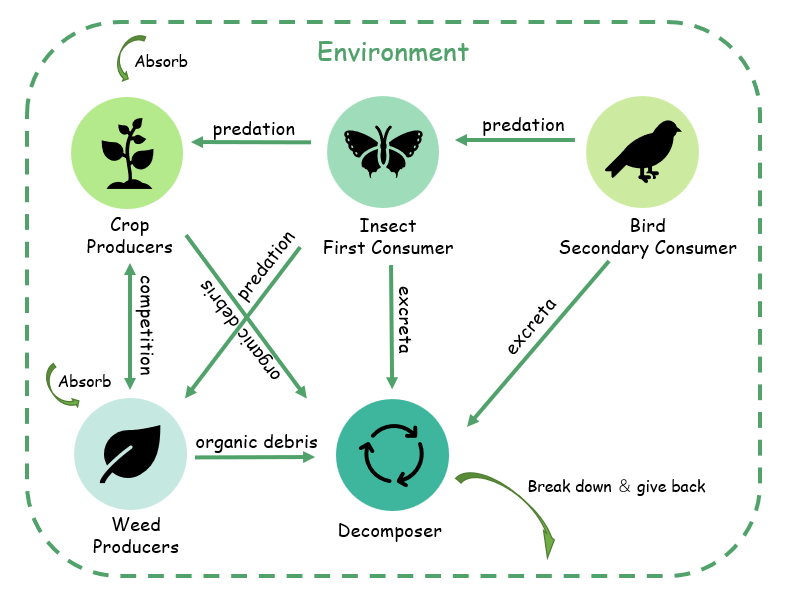
\includegraphics[width=0.395\textwidth]{./figures/elementary_ecosystem}
    \caption{Elementary Ecosystem Diagram}
\end{figure}

\textbf{For producers}, we classify them into crops and weeds. During natural cycle, The increase of biomass relies on photosynthesis, the decrease is made up of inter-specific competition, primary consumers' depletion and non-natural death. Chemical factors such as herbicides are analyzed in section 4.2. Hence, the dynamic equation for producers can be expressed as:
\begin{equation}
    \frac{dB_i}{dt}=r_iB_i(1-\frac{1}{K}\sum_{producer}B_k)-\beta_{pest-i}B_{pest}B_i-d_iB_i
    \label{original}
\end{equation}
where $r_i$ is the intrinsic productivity of crops or weeds, $d_i$ is crops' or weeds' mortality.
To better understand crop-weed competition, we modify the Logistic Equation and acquire:
\begin{equation}
    \begin{cases}
        \frac{dB_{crop}}{dt}=r_{crop}B_{crop}(1-\frac{B_{crop}}{K_{crop}}-\sigma_1\times \frac{B_{weed}}{K_{weed}})\\
        \frac{dB_{weed}}{dt}=r_{weed}B_{weed}(1-\frac{B_{weed}}{K_{weed}}-\sigma_2\times \frac{B_{crop}}{K_{crop}})
        \label{comp}
    \end{cases}
\end{equation}

\textbf{The consumers' perspective}. Pests, as primary consumers, increase by digesting consumers and decrease due to being preyed upon and respiration, which can be quantificationally expressed as:
\begin{equation}
    \frac{dB_{pest}}{dt}=r_{pest}B_{pest}(1-\frac{B_{pest}}{K_{pest}})+a_{pest-crop}B_{pest}B_{crop}+a_{pest-weed}B_{pest}B_{weed}-\beta_{bird-pest}B_{bird}B_{pest}
    \label{insect}
\end{equation}
where $r_{pest}$ is the respiration ratio of pests. Considering that in newly converted forest, ecosystems are uncomplicated,  so we can temporarily ignore the impacts of birds being preyed. Therefore we have:
\begin{equation}
    \frac{dB_{bird}}{dt}=r_{bird}B_{bird}(1-\frac{B_{bird}}{K_{bird}})+a_{bird-pest}B_{bird}B_{pest}
    \label{bird}
\end{equation}

Since \textbf{Decomposers} ($decomp.$ for short) feed on organic debris from producers, excreta from consumers and diminish owing to predators, we have equation \eqref{decomp.}. We as well assume that there already exists a finite amount of biomass, which will alter dynamically in a fashion demonstrated in figure \ref{Biomass}.
\begin{equation}
    \frac{dB_{decomp.}}{dt}=a_{decomp.-crop}B_{crop}+a_{decomp.-weed}B_{weed}+a_{decomp.-bird}B_{bird}-x_{decomp.}B_{decomp.}-\beta'
    \label{decomp.}
\end{equation}

\subsubsection{Impacts of Agricultural Cycle and Season}
\hspace{1.5em}We incorporate the significant impacts of agricultural cycles and seasonal transitions into system dynamics. To better illustrate our model, Region $Q$ is selected as our baseline, a city situated within the temperate monsoon climate zone of Northern Hemisphere. Winters in $Q$ feature harsh conditions, whereas summers marked by high temperature and precipitation. Cropping intensity in $Q$ allows for two harvests annually. These climatic conditions exert a significant influence on the biodiversity.
\begin{figure}[h]
    \centering
    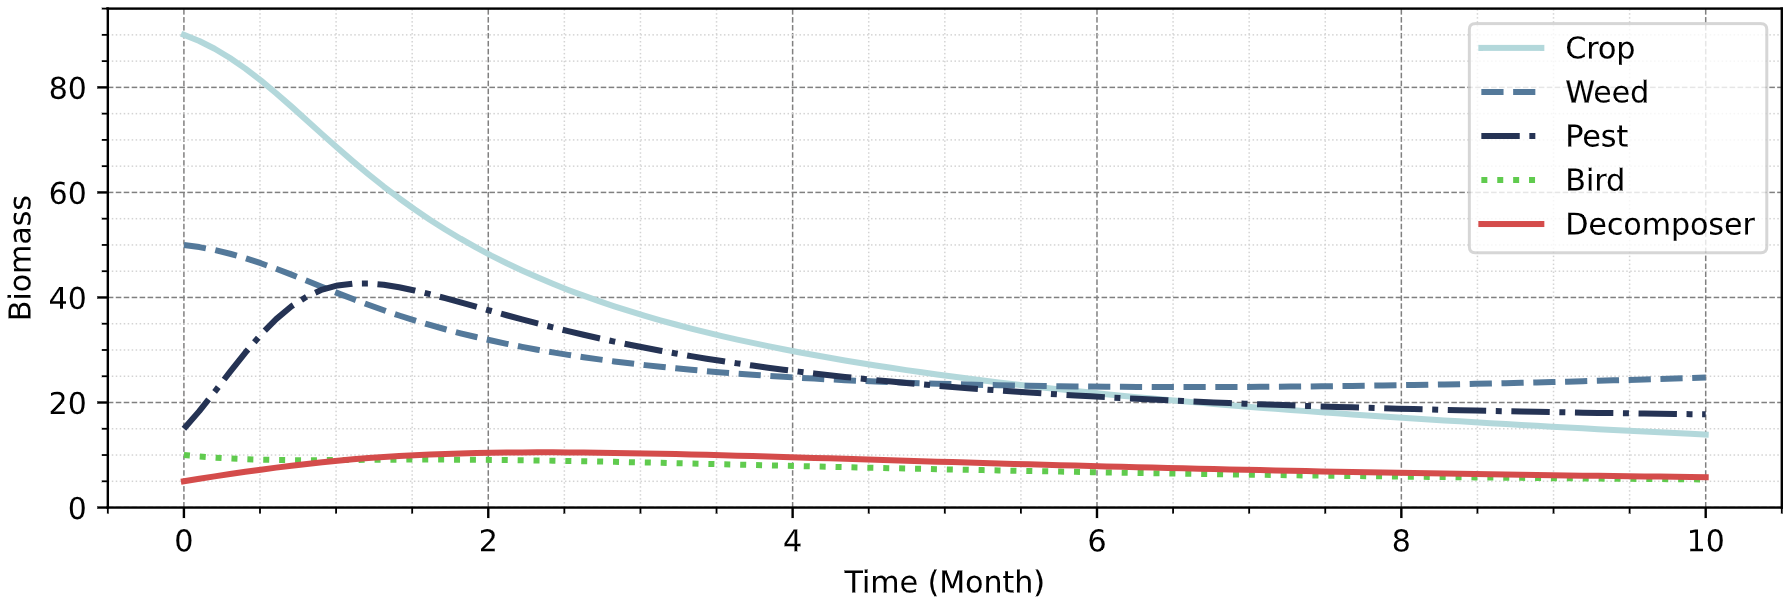
\includegraphics[width=0.8\textwidth]{./figures/biomass.png}
    \caption{Change of biomass without any intervention}
    \label{Biomass}
\end{figure}

To quantify the combined effects of multiple factors, we draw inspiration from the Superposition Principle in Circuits Analysis. Firstly, impacts of agricultural cycles and seasonal factors are set to zero to derive the relationship between population biomass and time. Then, only agricultural cycles and seasonal factors are considered to obtain the correlation between biomass and time. Finally, by summing these two relationships, we determine the comprehensive relationships between biomass and time. Considering agricultural cycles and seasonal factors, we describe the variation of biomass over time as $P_x(t)$.
\begin{equation}
    P_{x}(t)=P_{xmin}+k_{x}(P_{xmax}-P_{xmin})[1-A(t)]S(t)sin(\omega t+\phi)
\end{equation}

Then, we acquire the complete biomass of each ecosystem component as $C_{x}(t)$.
\begin{equation}
    C_{x}(t)=B_{x}(t)+P_{x}(t)
\end{equation}
where $x$ respectively represents ``crop'', ``weed'', ``pests'', ``birds'' or ``decomposers'', $k$ refers to the impact degree on diverse species, $A(\cdot)$ stands for agricultural tillage intensity, $S(\cdot)$ as seasonal impact factor index. Eventually, the complete biomass is calculated as follows:
\begin{equation}
    C(t)=C_{producers}(t)+C_{consumers}(t)+C_{decomposers}(t)
\end{equation}

To further calculate the biodiversity index for specified region, we substitute biomass values obtained from previous analysis into the \textbf{Shannon Index} formula (equation \eqref{shannon}). 
Additionally, the Shannon diversity index is standardized to finish subsequent calculations (formula \eqref{3}).
\begin{equation}
    H' = - \sum_{i=1}^{S} p_i \ln(p_i)
    \label{shannon}
\end{equation}
where $H'$ is the diversity index; $S$ represents the total species quantity and $p_i=\frac{Ci}{C}$ the relative richness of species $i$.
\begin{equation}
    E = \frac{H'}{H_{\max}'} = \frac{H'}{\ln(S)}
    \label{3}
\end{equation}

EEIM embodies significant practical meaning considering its visualization in figure \ref{shiboqi}. It can be observed that our model reaches its peaks in April and September, respectively in spring and autumn. Spring is the season to seed while autumn to harvest, both of which feature rich biodiversity. Additionally, between June and August, the crops begin to grow, nourishing numerous creatures in fields which ultimately contributes to increases in species richness. When the temperature drops in January, the biodiversity reaches its minimum level due to harsh living conditions. 
% 第一题的示波器
\begin{figure}[t]
    \centering
    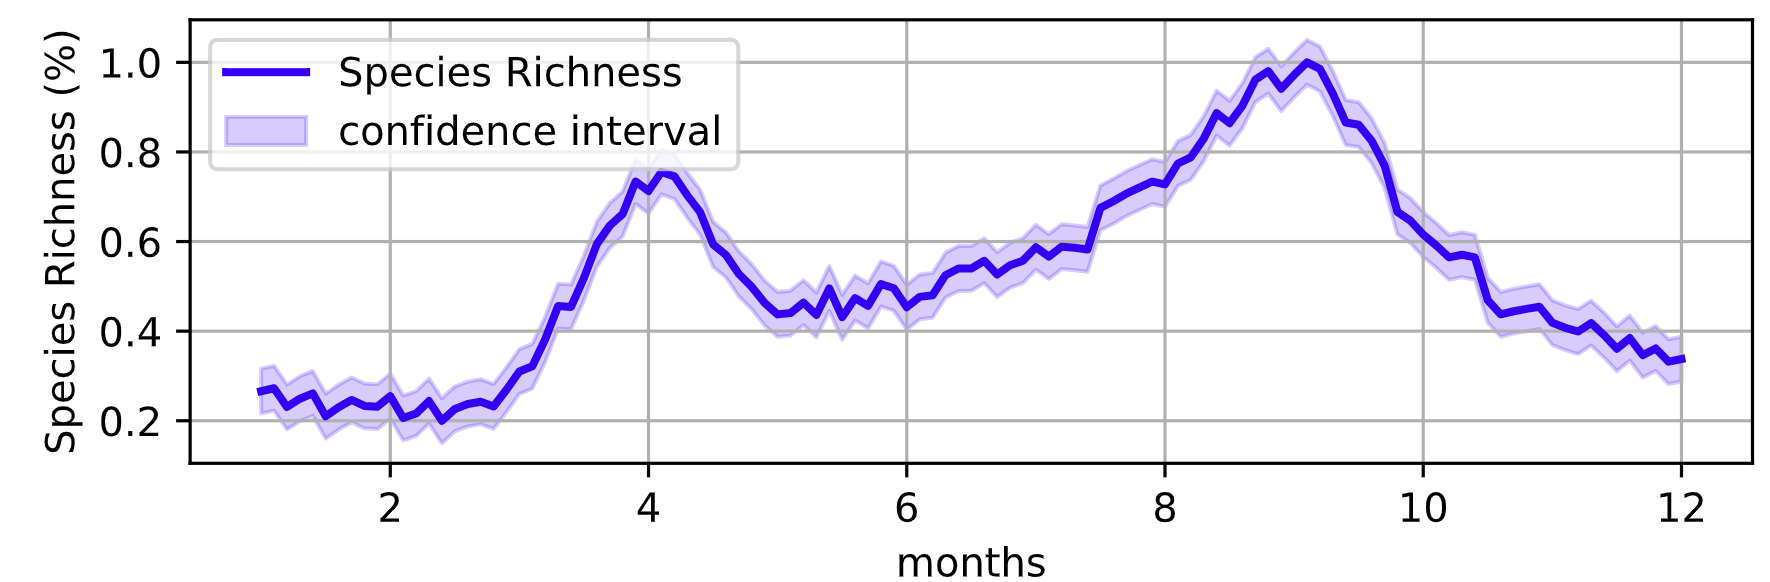
\includegraphics[width=0.7\textwidth]{./figures/basic_food_web_model_Species_Richness_Per_Year(task_1).png}
    \caption{Visualization of EEIM (in single year).}
    \label{shiboqi}
\end{figure}


\subsection{Elementary Ecology Destroyer Model, EEDM}
\hspace{1.5em}In section 4.1, we propose the EEIM to describe the food web under an ideal circumstance where chemical substances are excluded. In this section, we introduce the Elementary Ecology Destroyer Model (EEDM) to encompass humans' overuse of chemicals and corresponding negative effects on agricultural ecosystems. 
% 数据集构造思路
\begin{figure}[h]
	\centering
	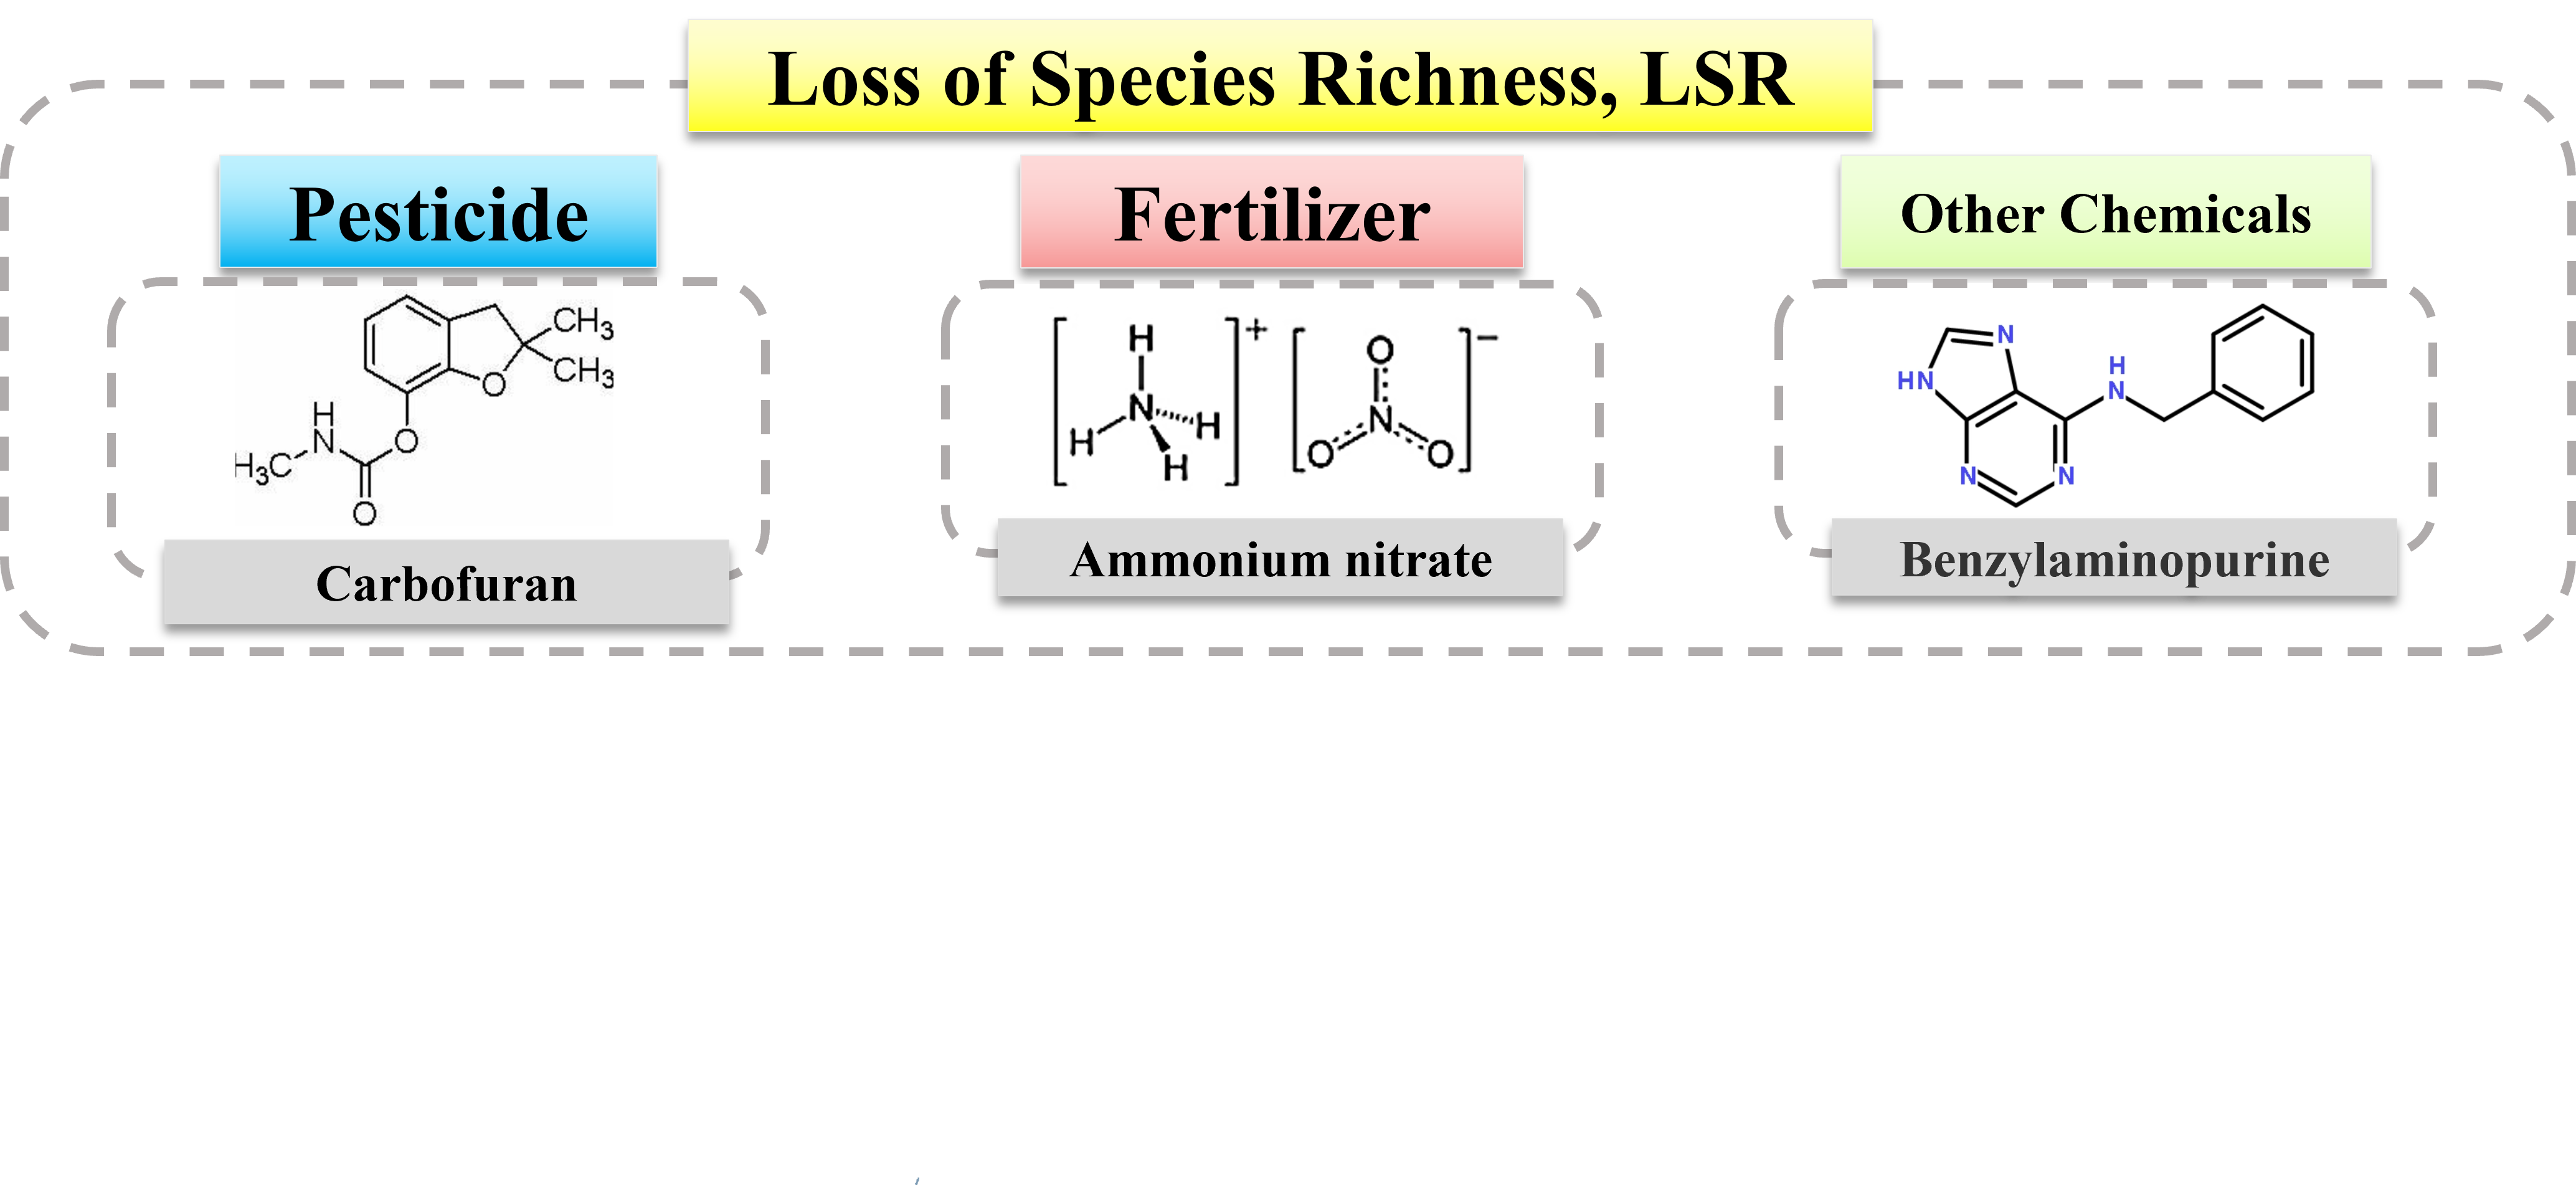
\includegraphics[width=0.8\textwidth,trim=0cm 6.2cm 0cm 0cm,clip]{./figures/dataset.png}
	\caption{Selected variables for the training dataset.}
	\label{dataset.}
\end{figure}

Researches have reported the complicated relationship between chemical usages and their corresponding effects. To simplify the process, we employ Multi-Layer-Perceptron (MLP) to better quantify the relationship between pivotal parameters and the loss of species richness ($LSR$). A rigorous procedure is followed to train our neural network, from dataset-preparation to robustness evaluation.


\textbf{Dataset Preparation. }Usages of pesticides ($Pest.$), fertilizers ($Fert.$) and other chemicals ($Oths.$) are selected to be the input features, since they are the major categories of agricultural chemicals. $LSR$ is chosen as the output label, illustrated in figure \ref{dataset.}. All the datas are collected from \cite{4}.
% MLP的构造思路
\begin{figure}[h]
	\centering
	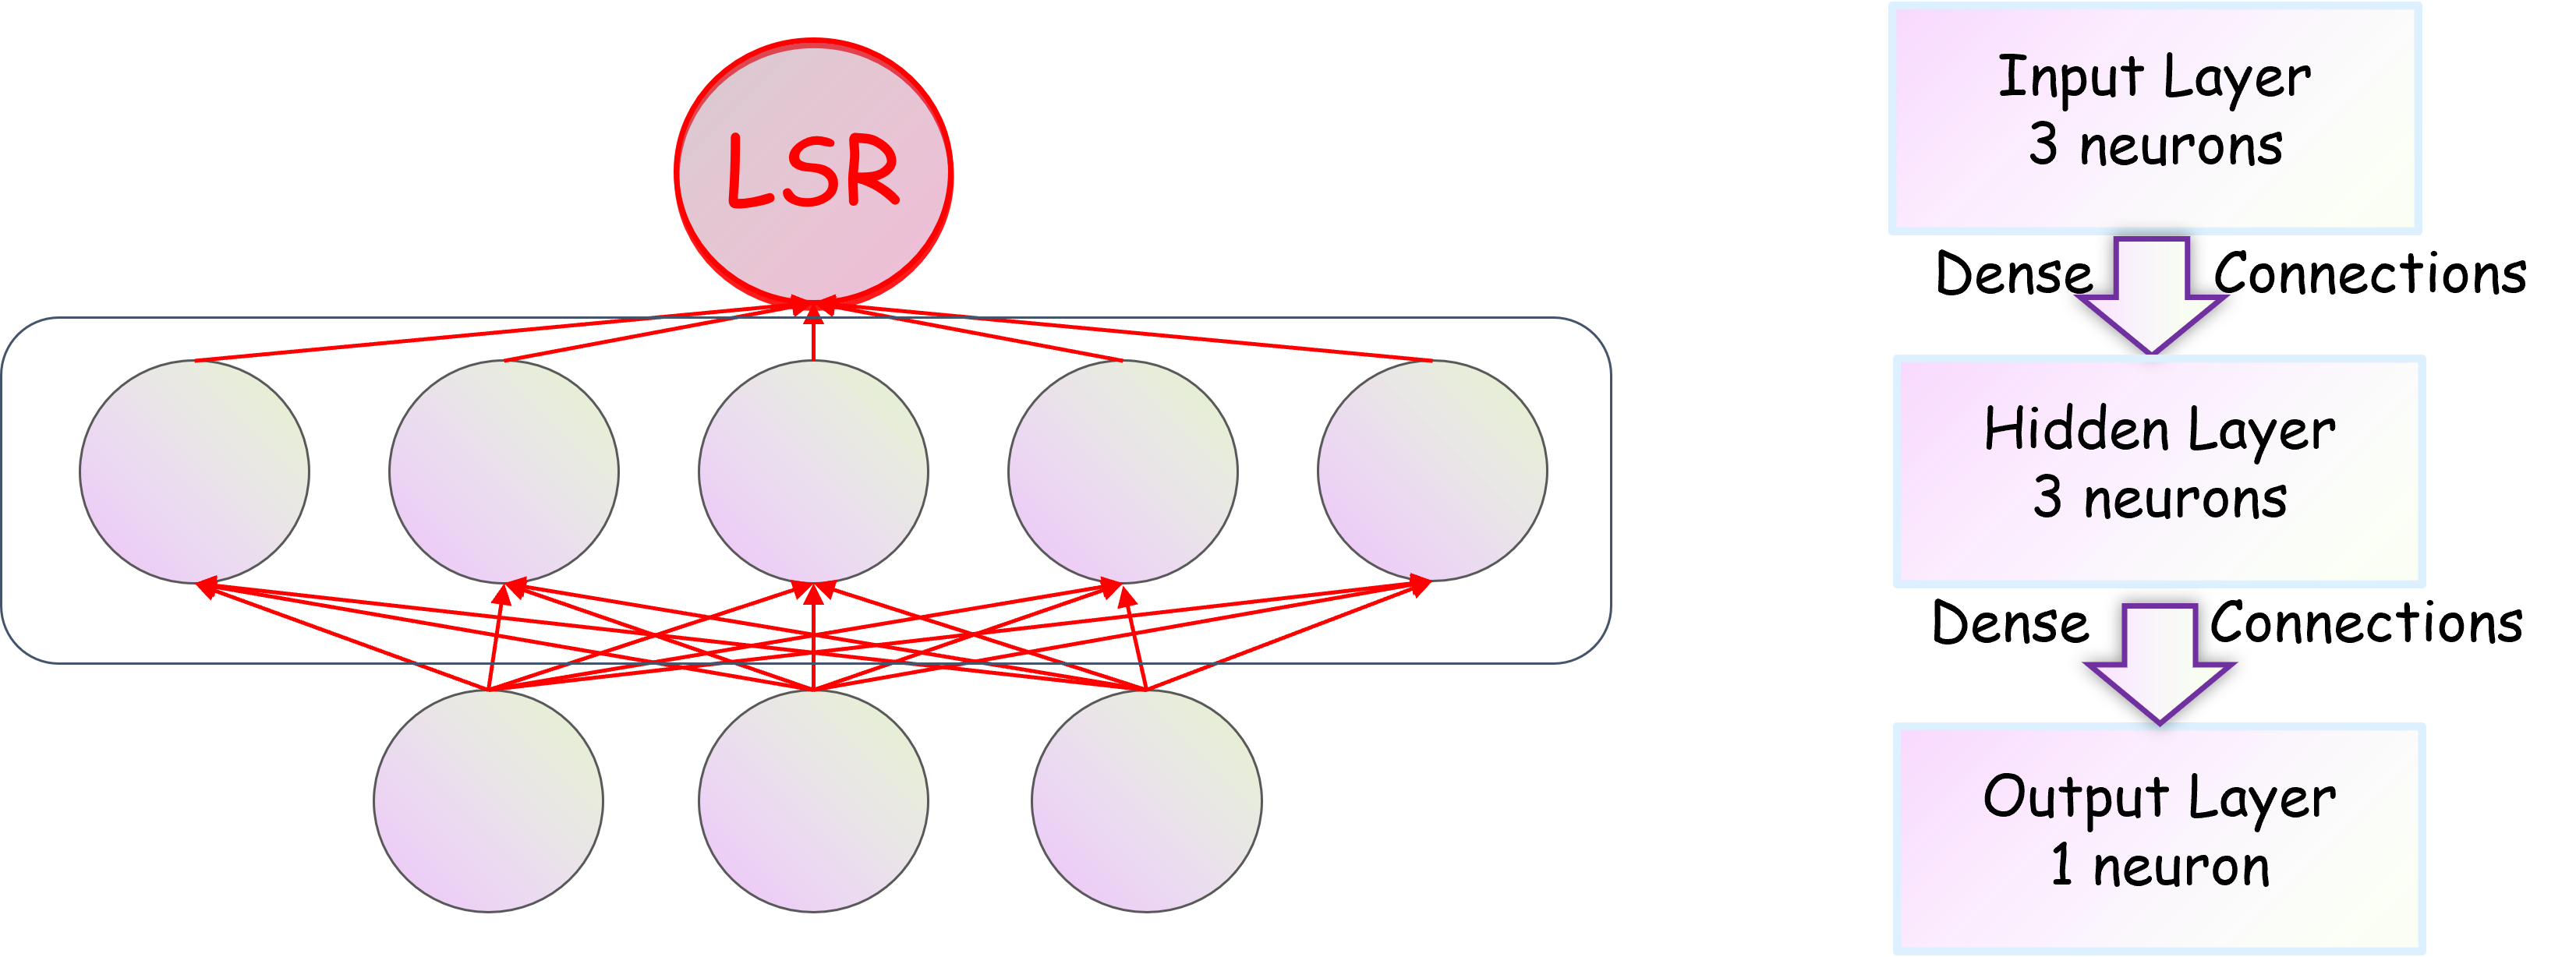
\includegraphics[width=0.6\textwidth]{./figures/MLP.png}
	\caption{Backbone MLP structure of the EEDM.}
	\label{MLP}
\end{figure}

\textbf{Experimental Configuration. }We applied one RTX 4060 GPU as hardware platform and the PyTorch Deep-Learning Framework. Mean Squared Loss (MSE) and Small Gradient Descents (SGD) are chosen as loss function and optimization algorithm (equation \ref{optimization}). Hyper-parameters are configured as: $batch\_size=16,\ epochs=125,\ learning\_rate=0.001$. Additionally, regularization techniques are employed to mitigate over-fitting: $dropout\_ratio=0.2$. Finally, we design a 3-3-1 neuron distribution for MLP (figure \ref{MLP}), which could be expressed as equation \ref{fp}, where $\textbf{W}_1\in\mathbb{R}^{3\times3},\textbf{W}_2\in\mathbb{R}^{1\times3},\textbf{b}_1\in\mathbb{R}^{3\times1},\textbf{b}_2\in\mathbb{R}^{1\times1},\sigma(\cdot)\in\mathbb{R}^{3\times3}$
% 损失函数和优化算法
\begin{equation}
	L(\textbf{w},b)=\frac{1}{n}\sum_{i=1}^{\mathbb{B}}\frac{1}{2}(\textbf{w}^T\textbf{x}^{(i)}+b-y^{(i)})^2,\hspace{0.3em}(\textbf{w},b)\leftarrow(\textbf{w},b)-\frac{\eta}{|\mathcal{B}|}\sum_{i\in\mathcal{B}}\partial_{(\textbf{w},b)}l^{(i)}(\textbf{w},b).
	\label{optimization}
\end{equation}
\begin{equation}
	LSR = \textbf{W}_{total}\cdot\textbf{X}+b_{total},\ \text{where}\ 
		\textbf{W}_{total} = \textbf{W}_2\cdot\sigma(x_i)\cdot\textbf{W}_1,\ 
		\textbf{b}_{total} = \textbf{W}_2\cdot\sigma(x_i)\cdot\textbf{b}_1 + \textbf{b}_2
	\label{fp}
\end{equation}

Through training (figure \ref{t}) we acquire $\textbf{W}_{total}=\begin{pmatrix}
    0.243 & 0.220 & 0.262
\end{pmatrix}$, $\textbf{b}_{total}=0.246$
and the original form of EEDM:
\begin{align}
LSR(\%) = 0.243\times Pest.(kg/ha) + 0.220\times Fert.(kg/ha) + 0.262\times Oths.(kg/ha) + 0.246
	\label{primitive}
\end{align}
where $LSR$ is the loss of species richness, $Pest.$, $Fert.$, $Oths.$ respectively stands for the quantity of used pesticides, fertilizers and other chemicals.
% 训练图
\begin{figure}[htbp]
	\centering
	\begin{subfigure}{0.46\textwidth}
		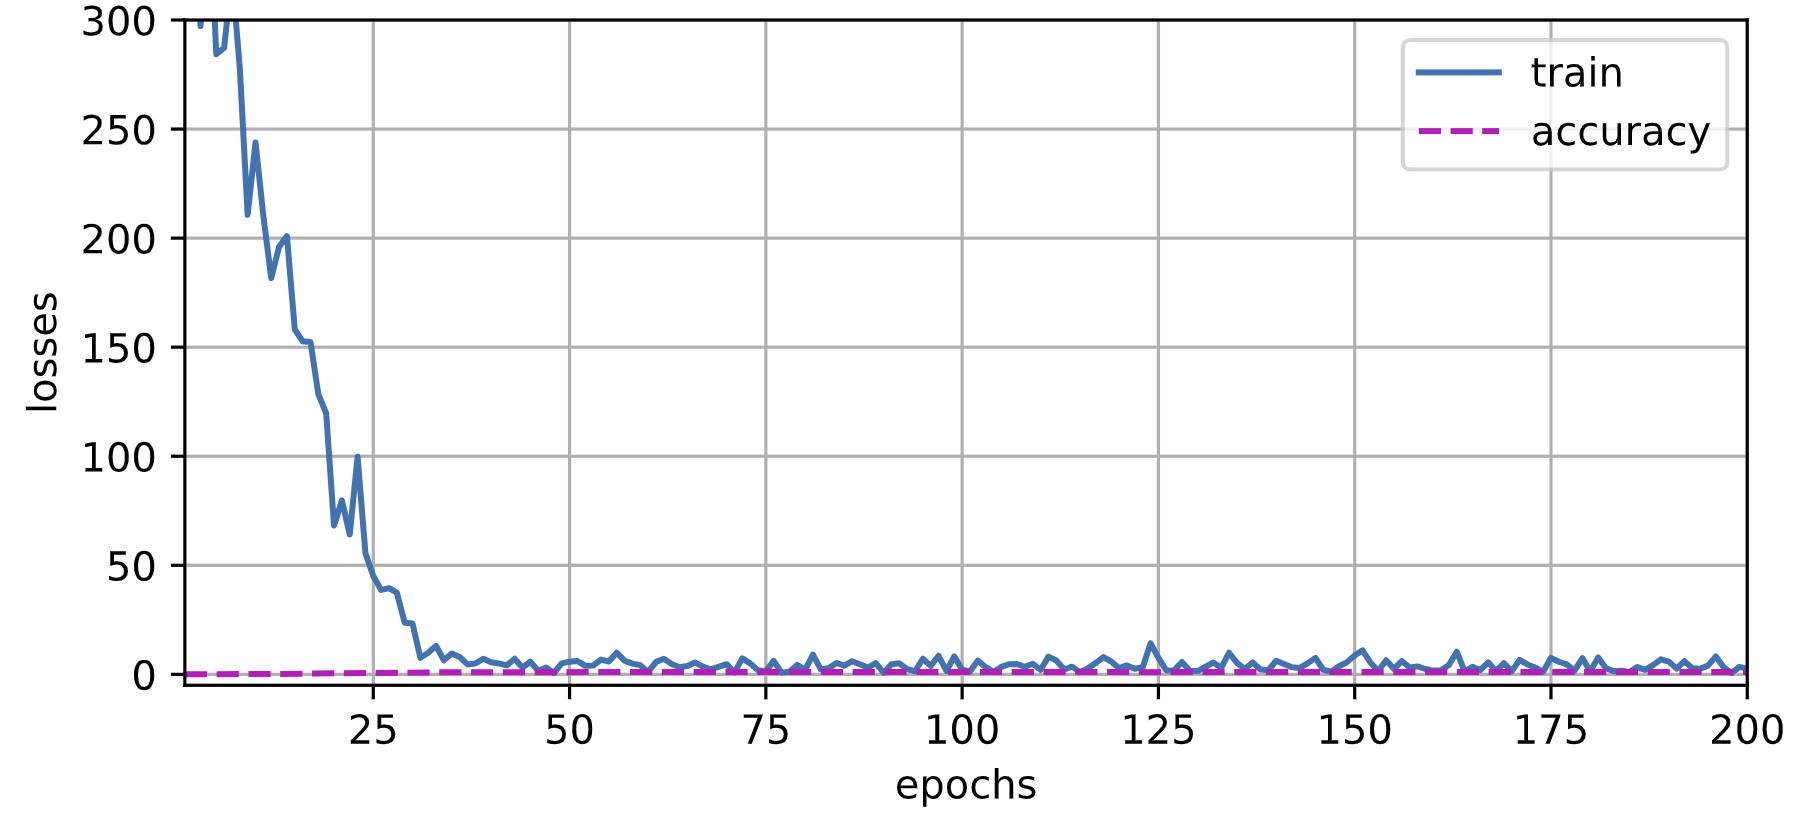
\includegraphics[width=\textwidth,trim=0cm 1.2cm 0cm 0cm,clip]{./figures/train.png}
		\label{train}
	\end{subfigure}
	\begin{subfigure}{0.46\textwidth}
		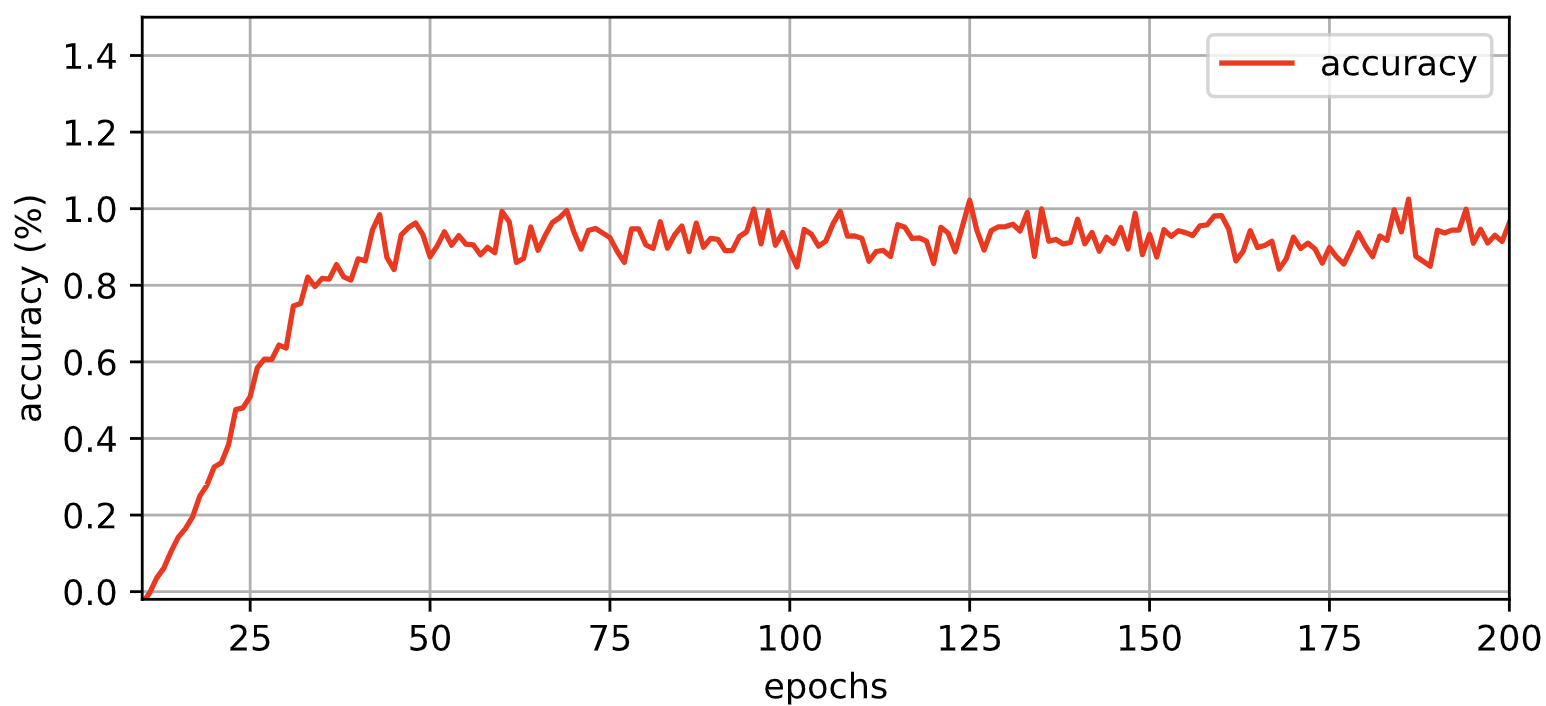
\includegraphics[width=\textwidth,trim=0cm 1.0cm 0cm 0cm,clip]{./figures/accuracy.png}
		\label{test}
	\end{subfigure}
	\caption{Our model-training process.}
	\label{t}
\end{figure}

A further transformation is conducted by mapping EEDM (equation \ref{primitive}) under temporal framework. Considering each of its sub-variables as functions correlated with time, we use \textbf{MATLAB} to fit each equation. We ultimately derive: $Pest.=-0.0012619\times t^2+5.1116424\times t-5176.717$, $Fert.=-0.06358907\times t^2+257.34633611\times t-260251.460$, $Oths.=-0.001238\times t^2+5.02035714\times t-5087.3170$, and a time-based EEDM (equation \ref{time}, figure \ref{ti}).
\begin{equation}
 LSR = -0.01462044487\times t^2+59.17365663\times t-59845.89449
	\label{time}   
\end{equation}

\begin{figure}[h]
	\centering
	\begin{subfigure}{0.44\textwidth}
	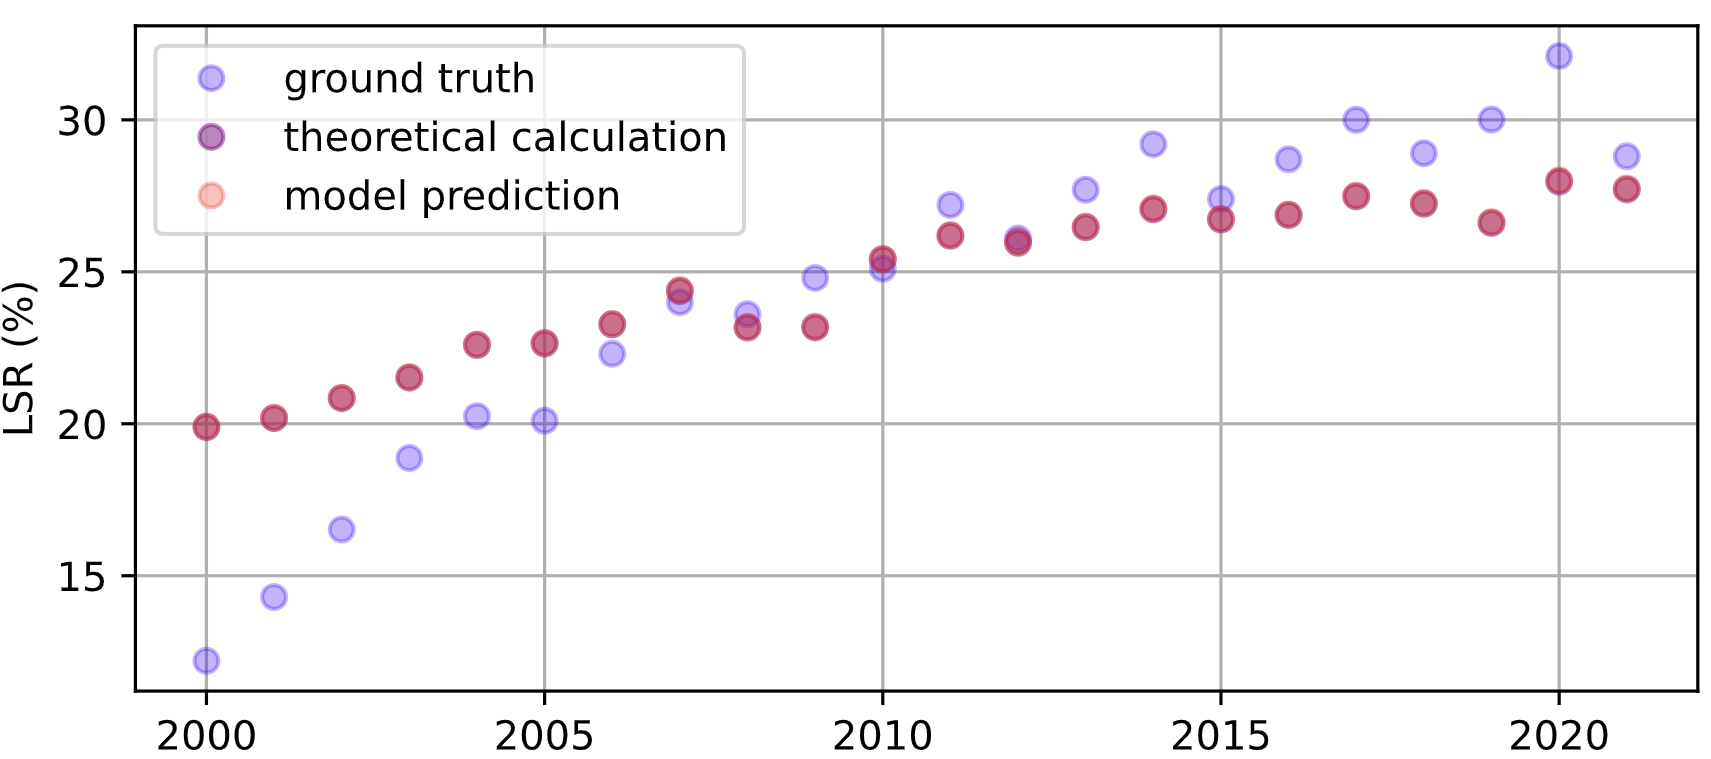
\includegraphics[width=\textwidth]{./figures/LSR_primitive_dimension.png}
\caption{Original Form.}
	\end{subfigure}
	\begin{subfigure}{0.46\textwidth}
		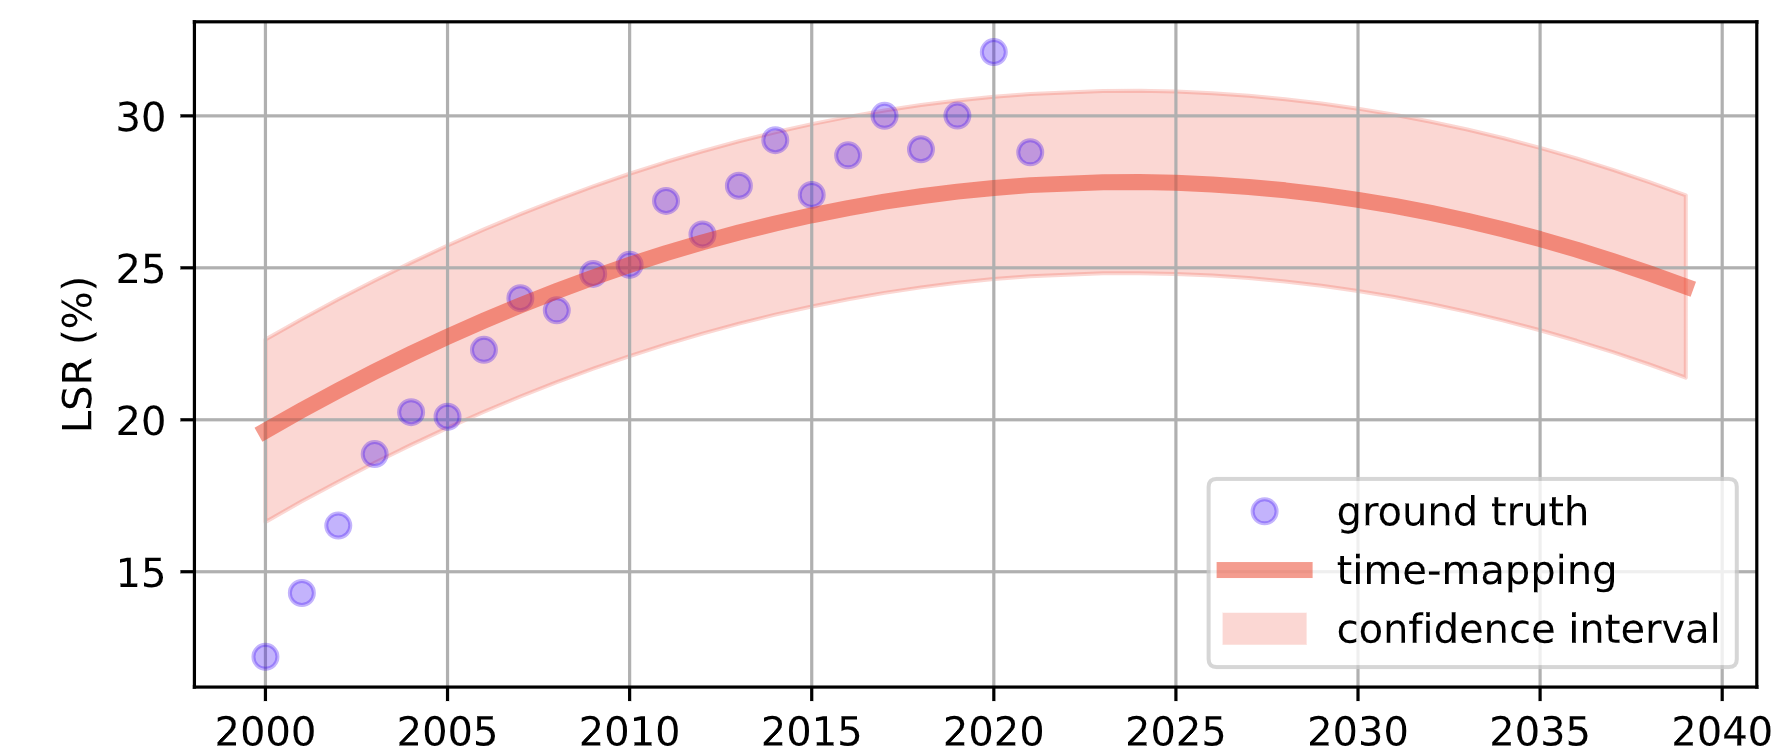
\includegraphics[width=\textwidth]{./figures/LSR_time_dimension.png}
		\caption{Temporal Form}
	\end{subfigure}
	\caption{Two forms of the EEDM: original and time-based respectively.}
	\label{ti}
\end{figure}

From figure \ref{t} it can be observed that our model reaches an accuracy of 91.3\% on validation dataset. We further verify our model by measuring the specific effects of chemical usages on birds population and the insects counterparts, as is illustrated in figure \ref{chemics}. It can be seen that overuse of chemicals contributes the greatest losses in plants richness, followed by pests, birds and other species. Such prediction aligns with reality since plants are the dominant creatures in agricultural ecosystems and insects are essential pollinators for crops.

\begin{figure}[h]
	\centering
	\begin{subfigure}[b]{0.36\textwidth}
		
\includegraphics[width=\textwidth,trim=0cm 1cm 0cm 0cm,clip]{./figures/chemics on eco(task 1).png}
		\caption{Agricultural ecosystem.}
		\label{hao}
	\end{subfigure}
	\begin{subfigure}[b]{0.45\textwidth}
		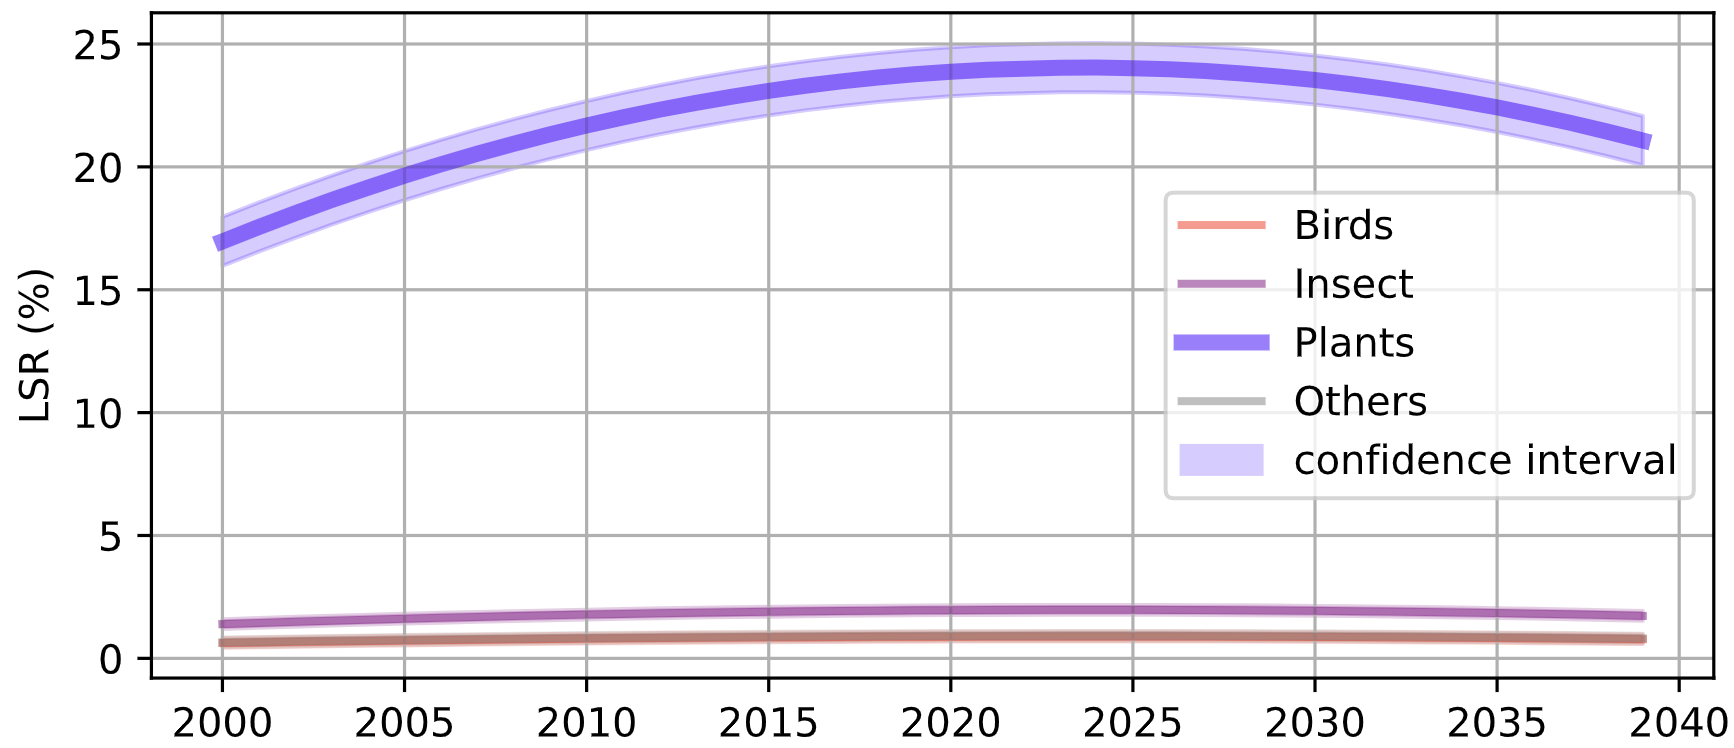
\includegraphics[width=\textwidth]{./figures/impacts_on_birds_etc(task 1)}
		\caption{Loss of species richness.}
	\end{subfigure}
	\caption{Effects of chemical usages on agricultural ecosystems, where datas in figure \ref{hao} stand for biomass proportions and are extracted from \cite{5}.}
	\label{chemics}
\end{figure}

\subsection{Food Web Model}
\hspace{2em}By combining EEIM and EEDM, we acquire the Food Web Model. Additionally, both sub-models exhibit dimensional consistency in calculated quantity while the mere difference lies in that EEIM calculates the species richness and EEDM the absolute value of lost richness caused by chemical usages. According to assumption 2, we define the Food Web Model as:\begin{equation}
	Food\ Web\ Model = EEIM - EEDM,\ \textbf{or}\ Stability/Richness=EEIM-EEDM
	\label{shiboqi_hetiban}
\end{equation}
where $Stability$ and $Richness$ are evaluated by a ratio regarding species biodiversity of unexploited regions as its baseline. From article \cite{4} we define ``unexploited regions'' as primary vegetation with low landscape cropland coverage and with minimal nitrogen fertilizer application rate (Zhao et al., 2024). Our 
Food Web Model is visualized by integrating figure \ref{shiboqi} and \ref{ti} on time-dimension referring to equation \eqref{shiboqi_hetiban}, as is illustrated in figure \ref{shiboqi_hetibian_detu}, where the shaded areas represent 95\% data confidence intervals and $Normalized\ Ratio$ stands for overall biodiversity ratio comparing to unexploited regions. Since the model takes all factors into consideration, it comprehensively reflects the primitive evolution dynamics of agricultural ecosystems and to what extent of damage humans have caused to existing regions. For instance, in figure \ref{shiboqi_hetibian_detu} we have $Total\ Species\ Richness=Net\ Species\ Richness-LSR$.
% 合体版示波器
\begin{figure}[h]
	\centering
	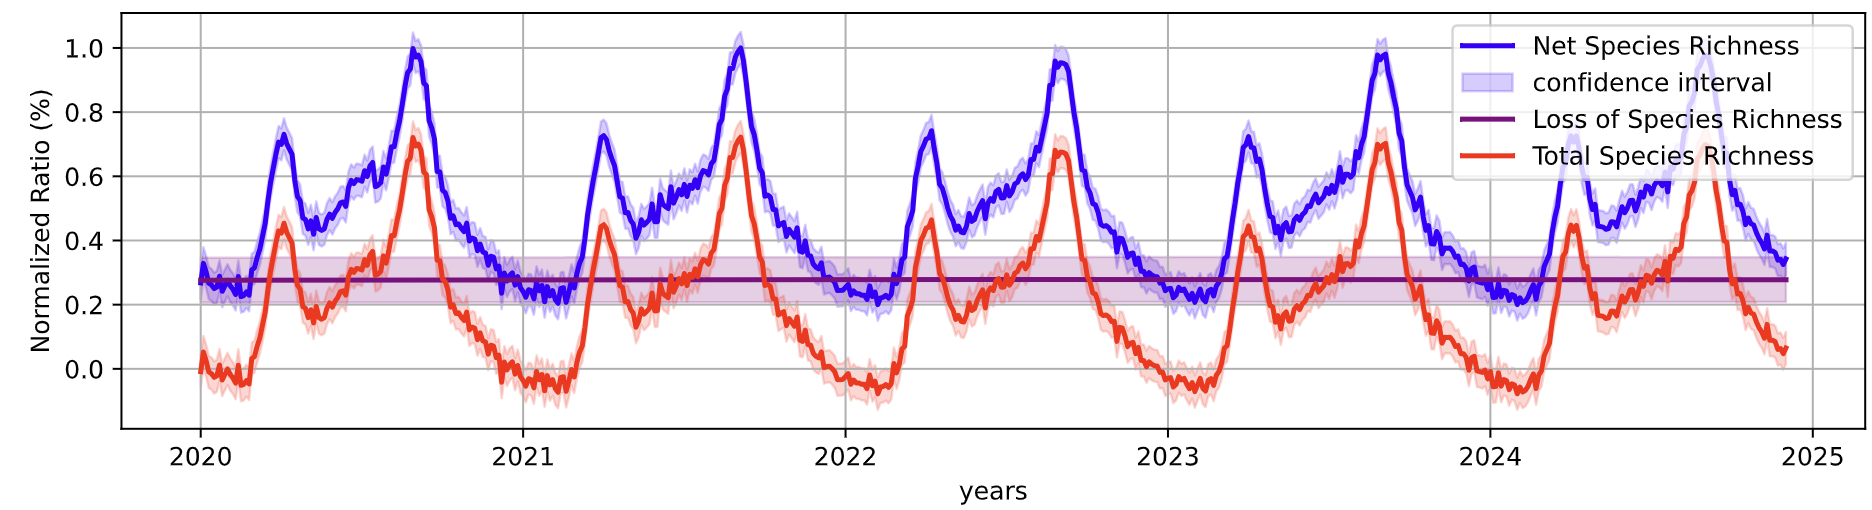
\includegraphics[width=0.95\textwidth]{./figures/shiboqi_hetiban(task1).png}
	\caption{Visualization of the Food Web Model.}
	\label{shiboqi_hetibian_detu}
\end{figure}



%%%%%%%%%%%%%%%%%%%%%%%%第二题
\section{Reemergence of native species}
\hspace{1.5em}Edge habitats sit in the buffer zone between farmlands and surrounding ecosystems. In this section, we propose the generalized Pascal's Triangle and Ecosystem Stability Model to evaluate impacts of native species' reemergence, which offer a dynamic view on the complete process of ecosystem evolution.
\subsection{Pascal's Triangle is all you need}
\hspace{1.5em}Native species are considered to have migrated into edge habits due to human exploits on the primary evolution stage of agricultural ecosystems. Therefore, they feature strong seasonal dynamics and geographical movements.

Pascal's Triangle is a triangular array of numbers widely used in algebra. Notice that the shape follows an increasing trend from inside out, we utilize this characteristic to demonstrate the geographical distributions of native species in terms of diverse evolution stages. By concatenating two triangles together into a square, we have the broadened Pascal's Triangle. For instance, equation \eqref{tong} provides a $4\times4$ triangle, which can be theoretically broadened to $n\times n$ dimension.
\begin{equation}
	\begin{matrix}
				& & & &1 & & & & \\
		& & &1&  &1& & & \\
		& &1& &2 & &1 & & \\
		&1& &3&  &3&  &1 & \\ 
	\end{matrix} \iff C(n,k)_x=C(n,k)_y=\frac{n!}{k!(n-k)!}\xrightarrow{ }\begin{pmatrix}
	C_x \\C_y
	\end{pmatrix}
	\label{tong}
\end{equation}

Similarly, by taking reciprocal on each value, we acquire another version of Generalized Pascal's Triangle which could explain the intermediate evolution periods when the majority of native species distribute in edge habitats: $\begin{pmatrix}
	\frac{1}{C_x} & \frac{1}{C_y}
\end{pmatrix}$. Visualization of both Pascal's Triangle is illustrated in figure \ref{tr}.
% 这是杨辉的两种形式
\begin{figure}[h]
	\centering
	\begin{subfigure}{0.25\textwidth}
		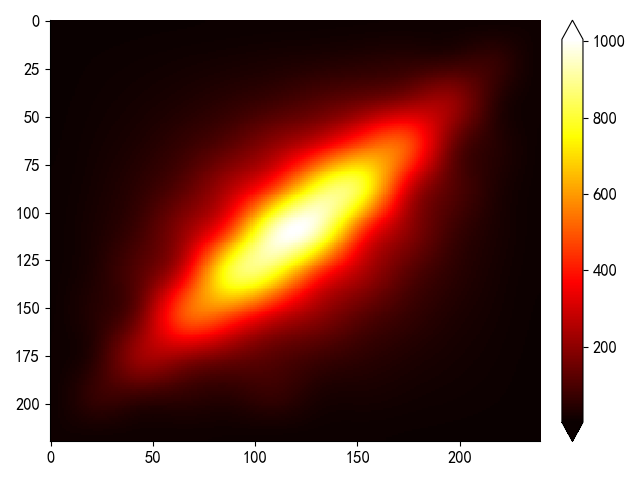
\includegraphics[width=\textwidth]{./figures/primitive triangle(task2).png}
		\caption{Original form.}
		\label{p}
	\end{subfigure}
	\begin{subfigure}{0.25\textwidth}
		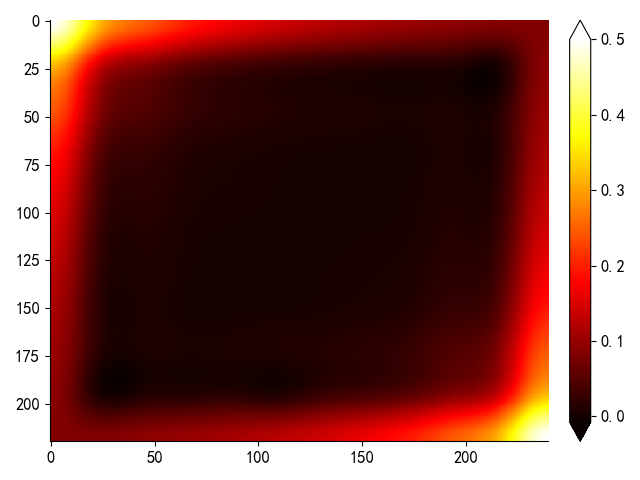
\includegraphics[width=\textwidth]{./figures/primitive reprocical triangle(task2)}
		\caption{Reciprocal form.}
		\label{wobuxiangxiele}
	\end{subfigure}
	\caption{Generalized Pascal's Triangle, where a brighter color indicates a larger species richness.}
	\label{tr}
\end{figure}

What differs figure \ref{p} and \ref{wobuxaingxiele} is their application scenarios. Figure \ref{p} describes the elementary stage of agricultural ecosystem evolution where the majority of native species distribute in central regions featuring sufficient living resources; Figure \ref{wobuxaingxiele} demonstrates the intermediate periods of evolution where the human exploits get involved and transform it into an agricultural ecosystem. Native species are accordingly compelled to migrate into edge habitats. 

\subsection{Impacts of Reemergence of Native Species}
\hspace{1.5em}The migration process is firstly simulated using our Generalized Pascal's Triangle. It's worth noting that, instead of choosing two specific species, we select symbolic creatures of two categories, namely $A$ and $B$, to generalize our model. Species $A$ is a native insect featuring dense population (such as \textit{Apis Mellifera}) while $B$ is a local animal with long lifespan but low population (such as \textit{Cervus Elaphus}). 

As is illustrated in figure \ref{mig}, the three stages of ecosystem evolution are demonstrated, including stage 1 (Natural Forest Area), stage 2 (Converted Agricultural System) and stage 3 (Mature Ecosystem). In stage 1, $A$ and $B$ settle in central regions; In stage 2, they migrate into edge habitats temporarily to escape human interference; In stage 3, due to a flourished and mature agricultural system, both species reemerge and relocate, sharing the living resources with human beings.
\begin{figure}[h]
	\centering
	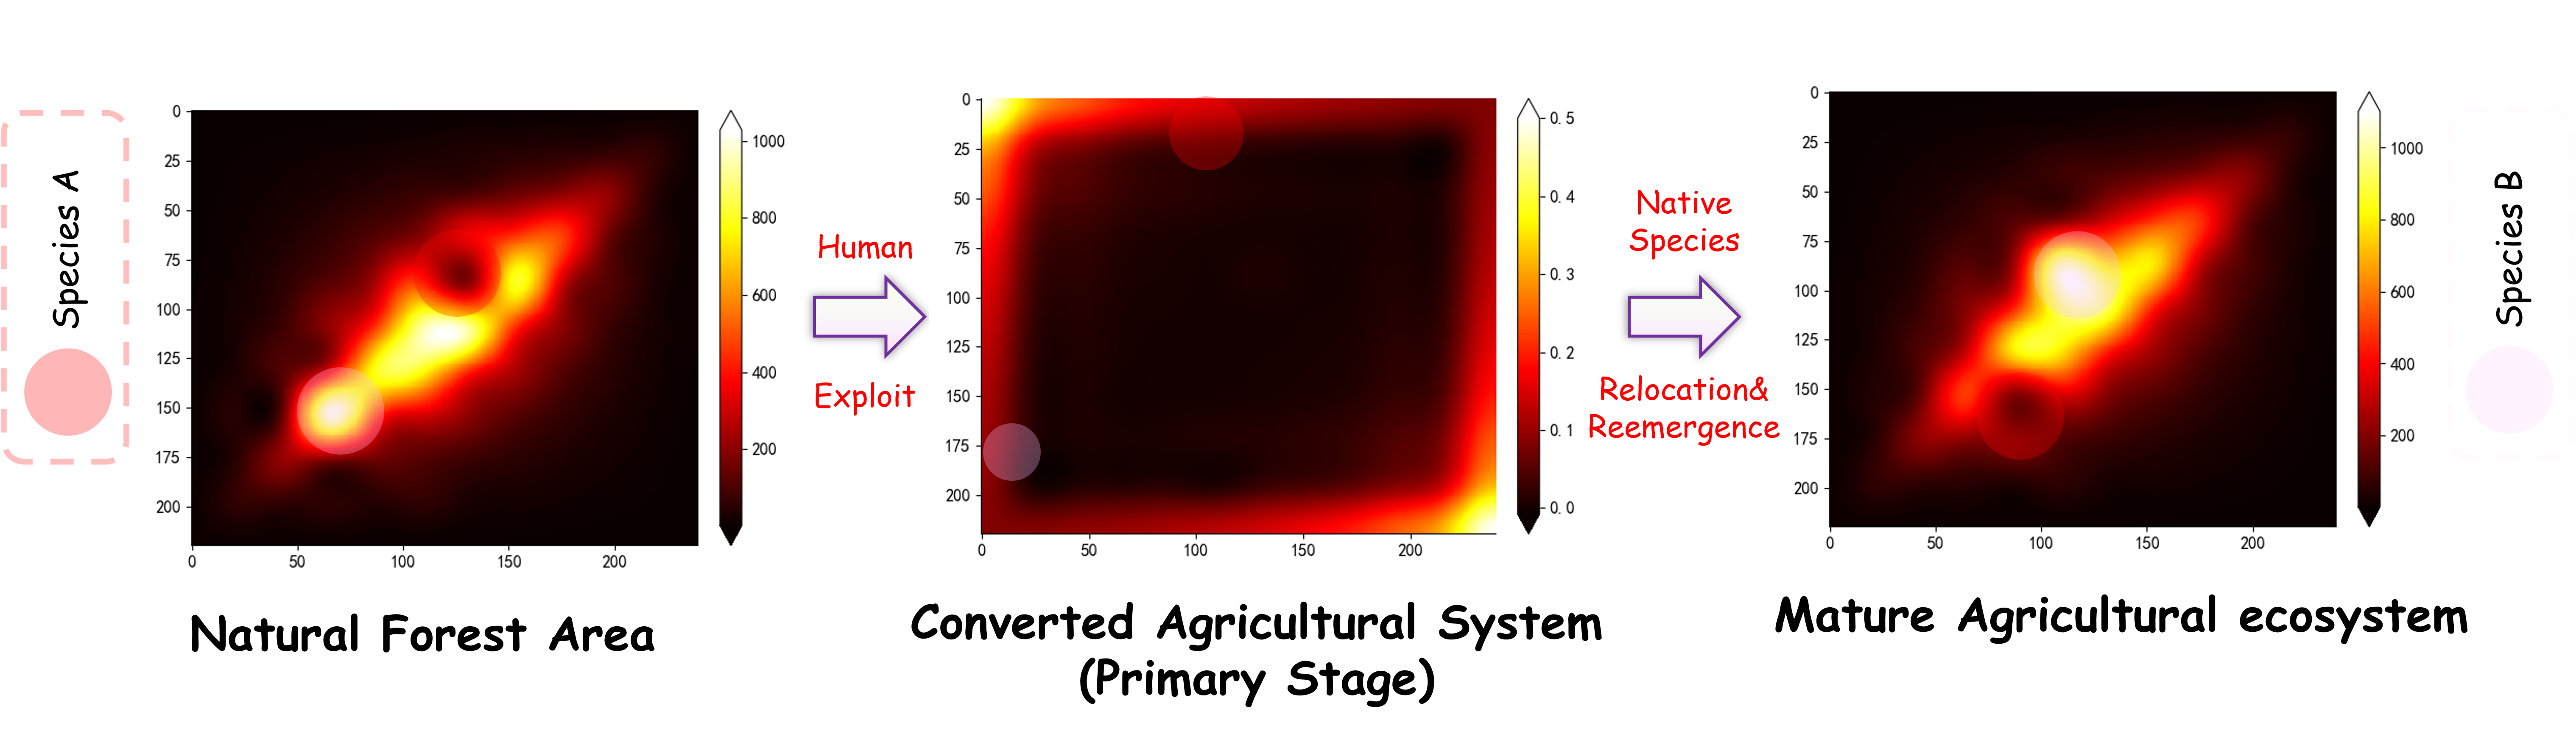
\includegraphics[width=\textwidth,trim=0cm 0cm 0cm 0.5cm,clip]{./figures/reemergence(task 2).png}
	\caption{A dynamic view of the three stages in ecosystem evolution and native species' reemergence.}
	\label{mig}
\end{figure}

While the Generalized Pascal's Triangle describes the dynamic reemergence of native species, the Ecosystem Stability Model (ESM) reveals the exact influence of species' reemergence on overall stability. ESM is composed of Resilience Stability ($RLS$) and Resistant Stability ($RTS$), both of which are correlated with species richness or diversity. Therefore, reemergence of  $A$ and $B$ benefits the ecosystem by impacting $RLS$ and $RTS$.

\begin{figure}[h]
	\centering
	\begin{subfigure}[b]{0.46\textwidth}
	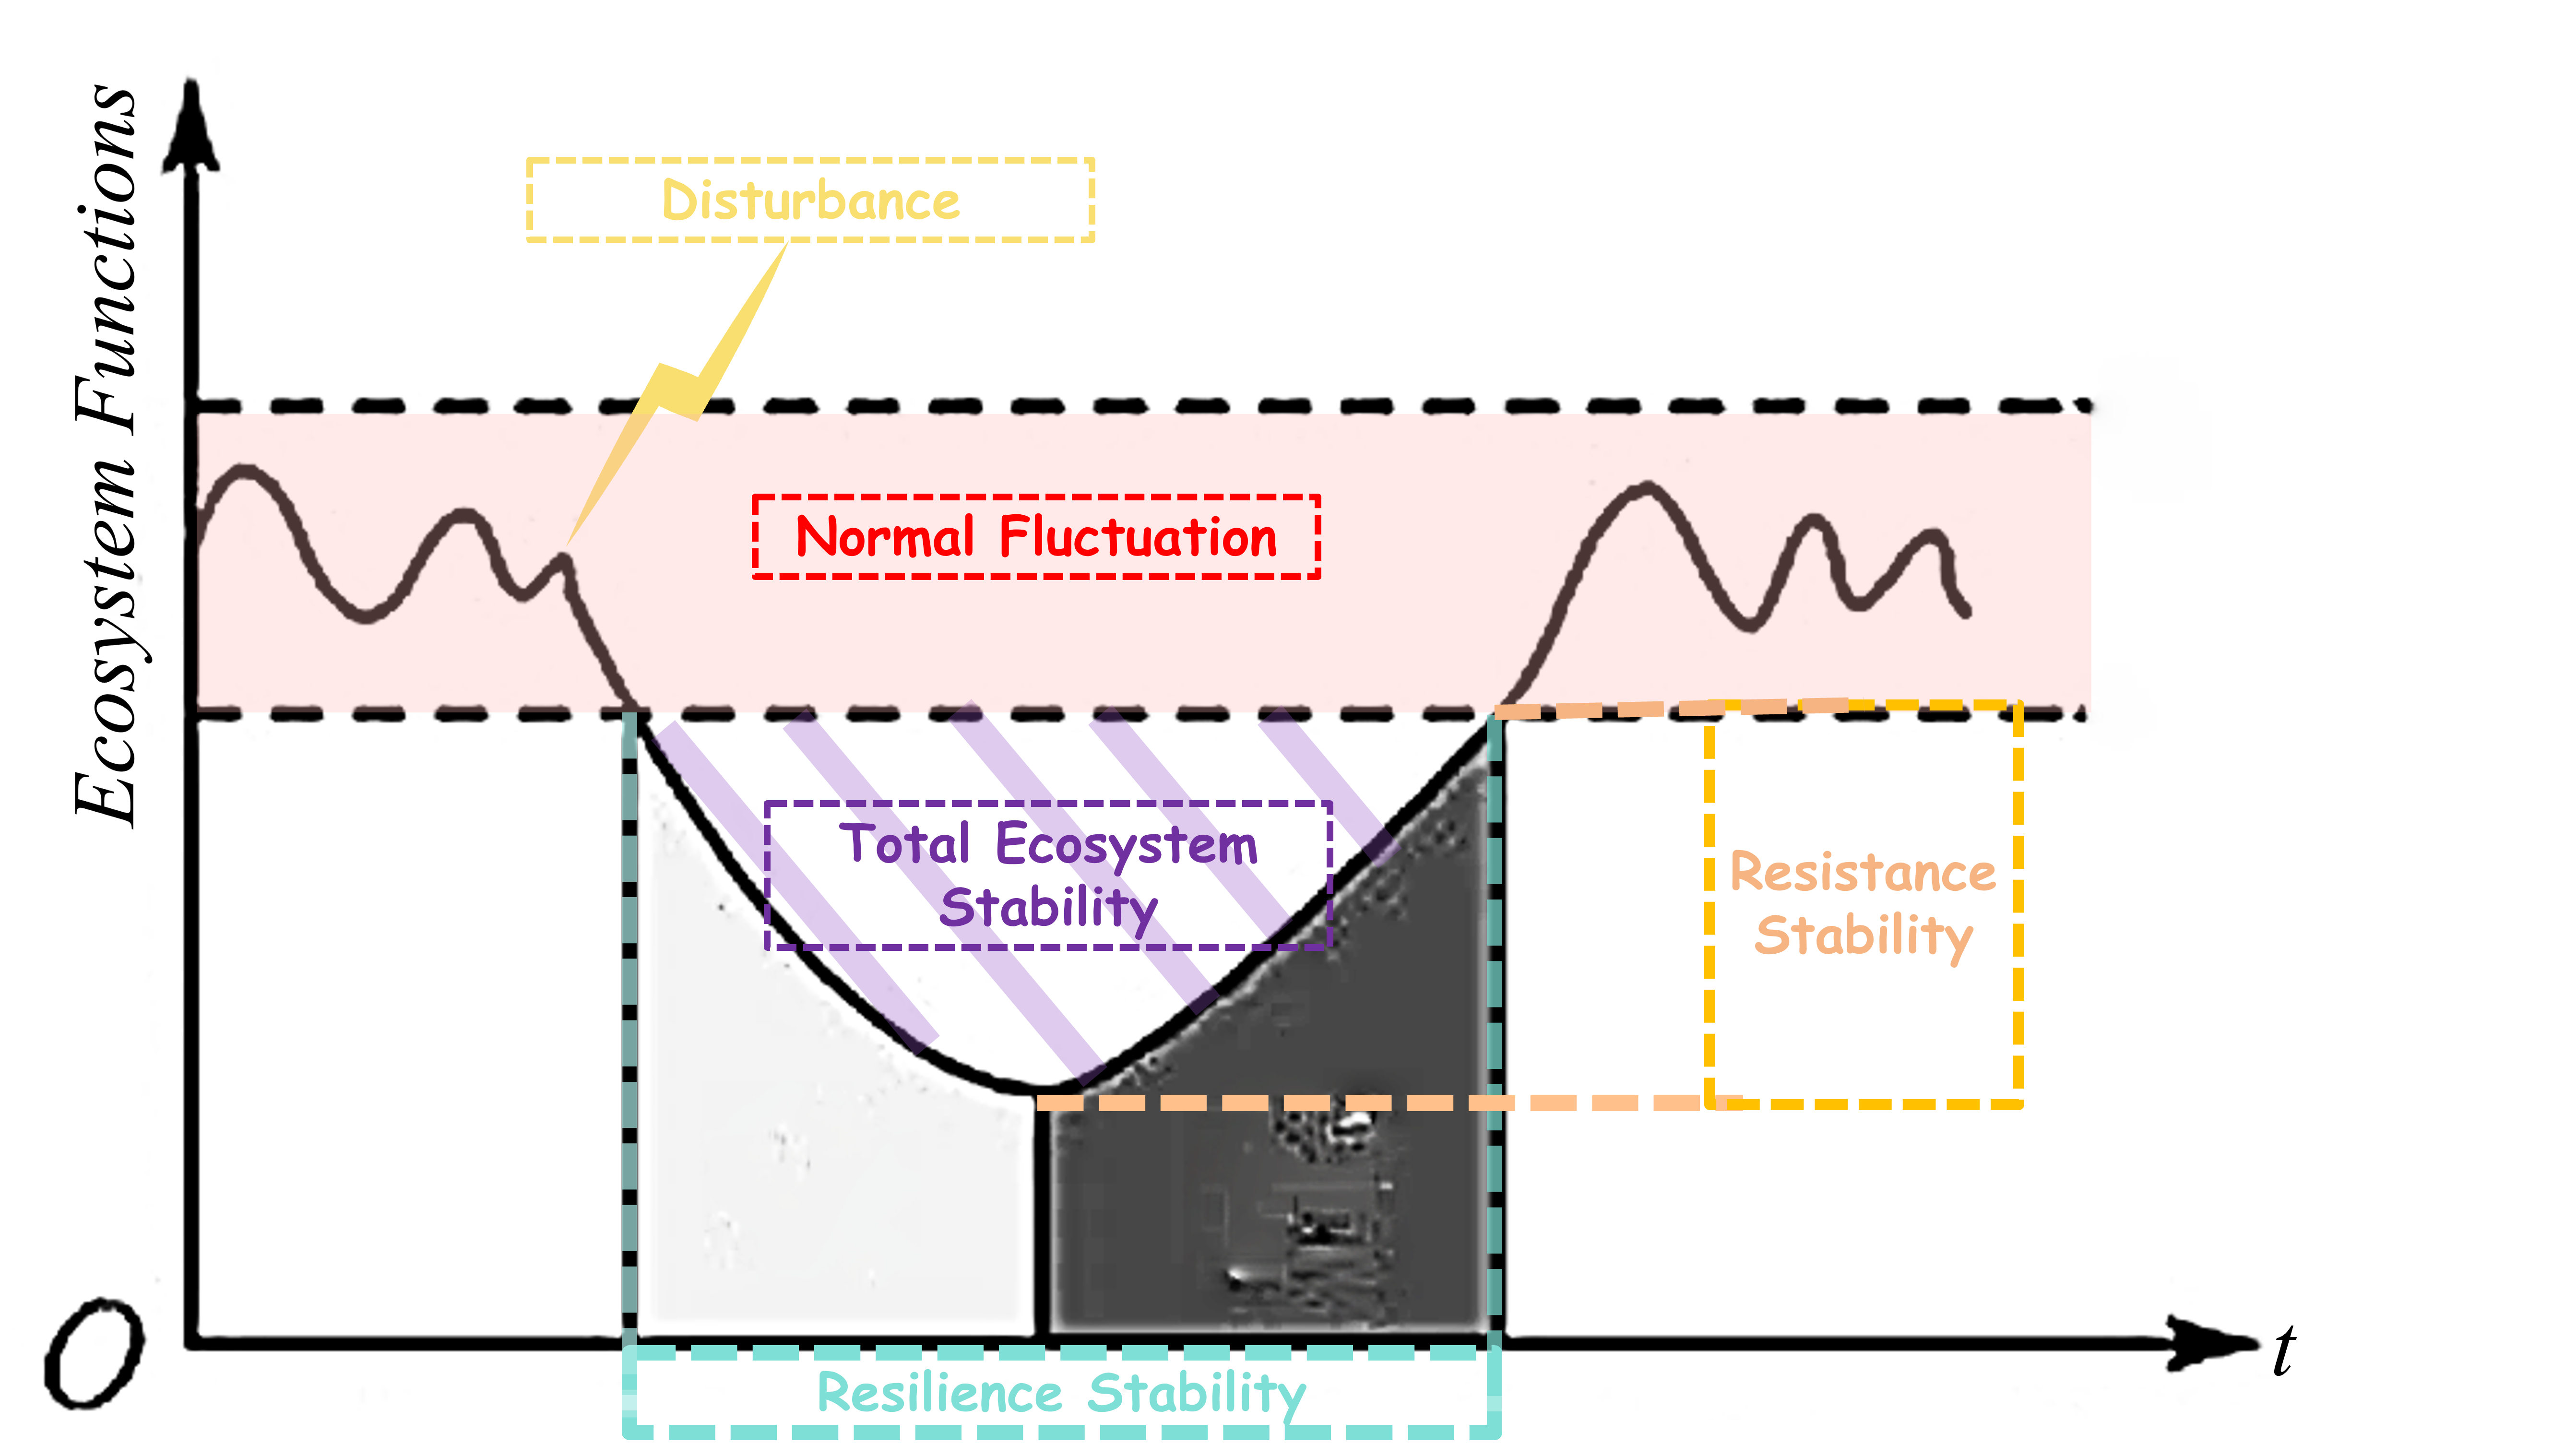
\includegraphics[width=\textwidth]{./figures/stability(task2).png}
	\caption{Ecosystem Stability Model (ESM).}
	\label{hhh}
	\end{subfigure}
	\begin{subfigure}[b]{0.37\textwidth}
		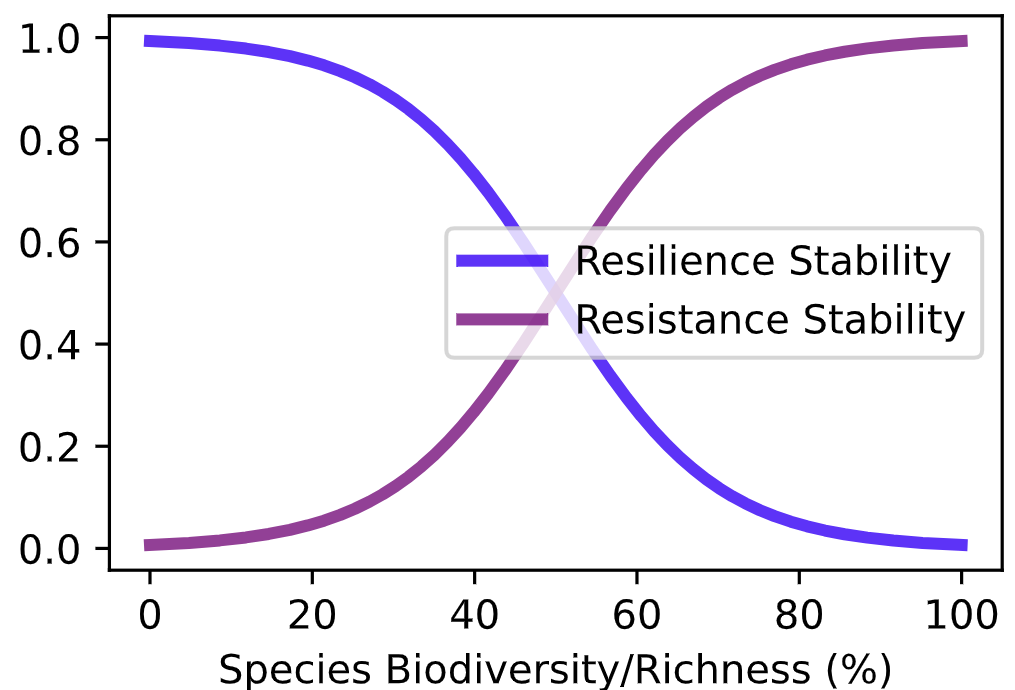
\includegraphics[width=\textwidth]{./figures/RSES(task 2).png}
		\label{x}
	\end{subfigure}
	\caption{Illustrations of the ESM Model.}
\end{figure} 

Let a sudden disturbance occur in ecosystem (given in figure \ref{hhh}). Define $Thresh_{min}$ as the minimum threshold of functional fluctuation in a stable ecosystem, while $F$ as ecosystems' function, $t_0$ and $t_1$ respectively the first, second time when $Thresh_{min}=F$. Therefore we have:
\begin{equation}
\begin{cases}
	TES = \int_{t_0}^{t_1}(Thresh_{min}-F) \\
	RTS = Thresh_{min} - \min{F},\ 	RLS = t_1 - t_0
\end{cases},\text{and}\ \begin{cases}
	Stability \propto \frac{1}{TES} \\
	RTS \propto Richness,\ 	RLS \propto \frac{1}{Richness}
\end{cases}
\label{rts}
\end{equation}

Assign $Richness_{before}$ to represent species richness before the reemergence of $A$ and $B$, while $Richness_{after}$ the opposite. Obviously we have: $Richness_{after}>Richness_{before}$, considering $Thresh_{min}$ as a constant, we have:
\begin{align*}
& 	RTS_{after}>RTS_{before},RLS_{after}<RLS_{before}  \xrightarrow{ }
	F_{after}>F_{before},
	(t_1-t_0)_{after}<(t_1-t_0)_{before} \\
& \xrightarrow{ }TES_{after}<TES_{before}\xrightarrow{ } Stability_{after}>Stability_{before}
\end{align*}

Therefore, we reach to the conclusion that reemergence of species $A$ and $B$ improved the overall stability of mature agricultural ecosystem. Additionally, our model explains the inner mechanism on detailed processes of how native species migrate during different evolution stages, offering new insights into animal-behavior-related ecosystem researches.

%%%%%%%%%%%%%%%%%%%%%%第三题
\section{Consequences of the Herbicide Removal}
\hspace{1.5em}As agricultural ecosystems mature, food webs become much more complex, and pests gradually develop resistance to pesticides. Consequently, farmers tend to reduce the use of chemicals. 
	
The reduction on herbicide may seem to provide a more stable ecosystem, from our analysis, however, it is not always the case. Time periods of herbicide removal have to be considered. In the short term, chemical reduction undoubtedly leads to higher richness (section 6.1.1) and stronger resistance (section 6.1.2). Oppositely, for the long run, reduction on chemicals may flourish weeds that are powerful competitors against crops in terms of finite nutrients. Under such circumstances, species richness may decline to its minimum quantity. Therefore, bats are introduced (section 6.2), which we call as ``the Biological Control''.
	\subsection{A Stable Ecosystem---A short term analysis}
	\subsubsection{Higher Richness}
\begin{figure}[h]
	\centering
	\begin{subfigure}{\textwidth}
		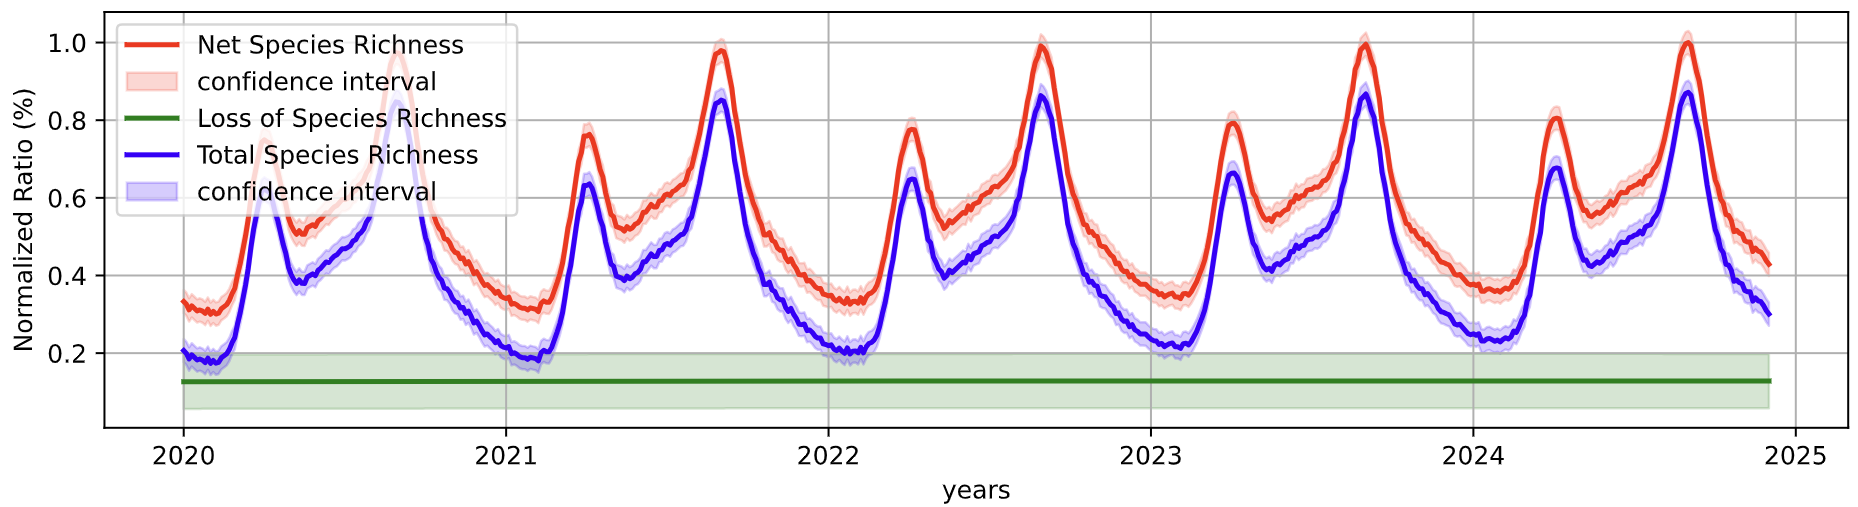
\includegraphics[width=0.9\textwidth, trim=0cm 0.5cm 0cm 0cm,clip]{./figures/shiboqi_hetiban(task3).png}
		\caption{Net \& Total Species Richness after herbicide removal.}
		\label{tk}
	\end{subfigure}
	\begin{subfigure}{\textwidth}
		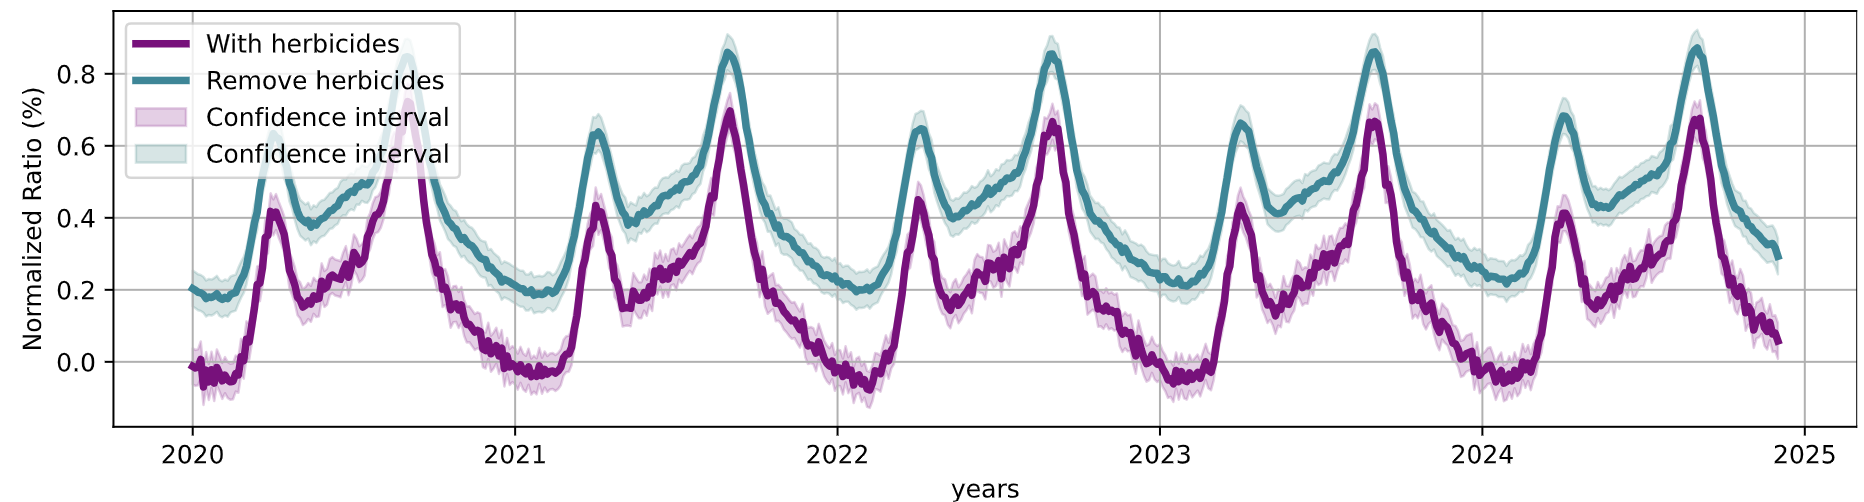
\includegraphics[width=0.9\textwidth,trim=0cm 0.6cm 0cm 0cm,clip]{./figures/shiboqi_Task3(1).png}
		\caption{Comparisons on total species richness before and after herbicide removal.}
		\label{2}
	\end{subfigure}
	\caption{Effects of herbicide removal on ecosystem stability and species richness.}
	\label{sbq}
\end{figure}
\hspace{1.5em}From the perspective of producers, when herbicide is removed, the growth rate of weeds will evidently increase, leading to a greater diversity of plant species. Additionally, the reduction in harmful chemicals entering soil promotes proliferation of soil microorganisms, enhancing fertility, boosting crop yields and the maximum environmental carrying capacity. However, increases in insect populations may cause limitations on plant growth, eventually reaching a new state of equilibrium. Therefore, equation \eqref{original} is optimized as: 
\begin{equation}
	\frac{dB_i}{dt}=\alpha_iB_i(1-\frac{1}{W}\sum_{producer}B_k+\theta_i)-f_{pest-i}B_{pest}B_i-\beta_iB_i
	\label{modified}
\end{equation}
where $\theta_i$ represents the growth-promoting effect of soil microorganisms on species $i$, and $\alpha_i=1.285r_i$, $W=1.697K$, $f_{ins-i}=1.276a_{ins-i}$, $\beta_i=0.649d_i$.

However,the aggressive spread of weeds will compete with crops for vital resources (e.g., water), resulting in substantial stress on crop growth. Therefore, \eqref{comp} is revised and we define  $q=\frac{\sigma_1}{\sigma_2}$   as the relative competition coefficient between weeds and crops. It is concluded that $q$, in the short term, initially increases over time, then decreases and finally stabilizes. This indicates that after the cessation of pesticide use, weeds exhibit a stronger competitive ability compared to crops, leading to vigorous growth. Subsequently, due to resource limitations in the environment, their competitive ability diminishes and eventually stabilizes. Yet still, the initial growth of weeds contributes to the biodiversity of the ecosystem.

From the perspective of consumers,  enhancements of plant diversity and biomass provides animals with richer food resources. The reduction of pesticide use has led to a significant increase in primary consumers' quantity, which in turn promotes the growth of secondary consumers. In other words, $r_{insects}$ and $r_{bird}$ will respectively increase in the formula \eqref{pest} \eqref{bird}. Additionally, diverse vegetation structures offer more complex habitats for various animal species, which contribute to the stable growth of animal populations. Overall improvements of ecological environment attract more species into the ecosystem, forming a more intricate food web. Such increased complexity significantly enhances the stability and resistance of ecosystems.

We further visualize the impacts of herbicides (and other chemical substances) removal by recalculating total species richness and aforementioned metrics referring to equation \eqref{shiboqi_hetiban}, with the results shown in figure \ref{sbq}. From figure \ref{tk} it can be concluded that, $LSR$ triggered by overuse of chemicals are mitigated but still having negative effects on ecosystem stability, while figure \ref{2} demonstrates that herbicide removal could directly contribute to higher biodiversity and stability, where the minimum value has been elevated to 19.8\%.

\subsubsection{Stronger Resistance}
\hspace{2em}According to equation \eqref{rts}, we conclude that biodiversity and species richness is positively proportional to ecosystem stability. Additionally, in formula \eqref{modified} we optimize \eqref{original} and infer the removal of herbicides positively facilitates biomass and biodiversity of either producers or consumers, indicating an increase in resistance stability and a decrease in resilience stability, as is illustrated in figure \ref{resistance}

\begin{figure}[h]
	\centering
	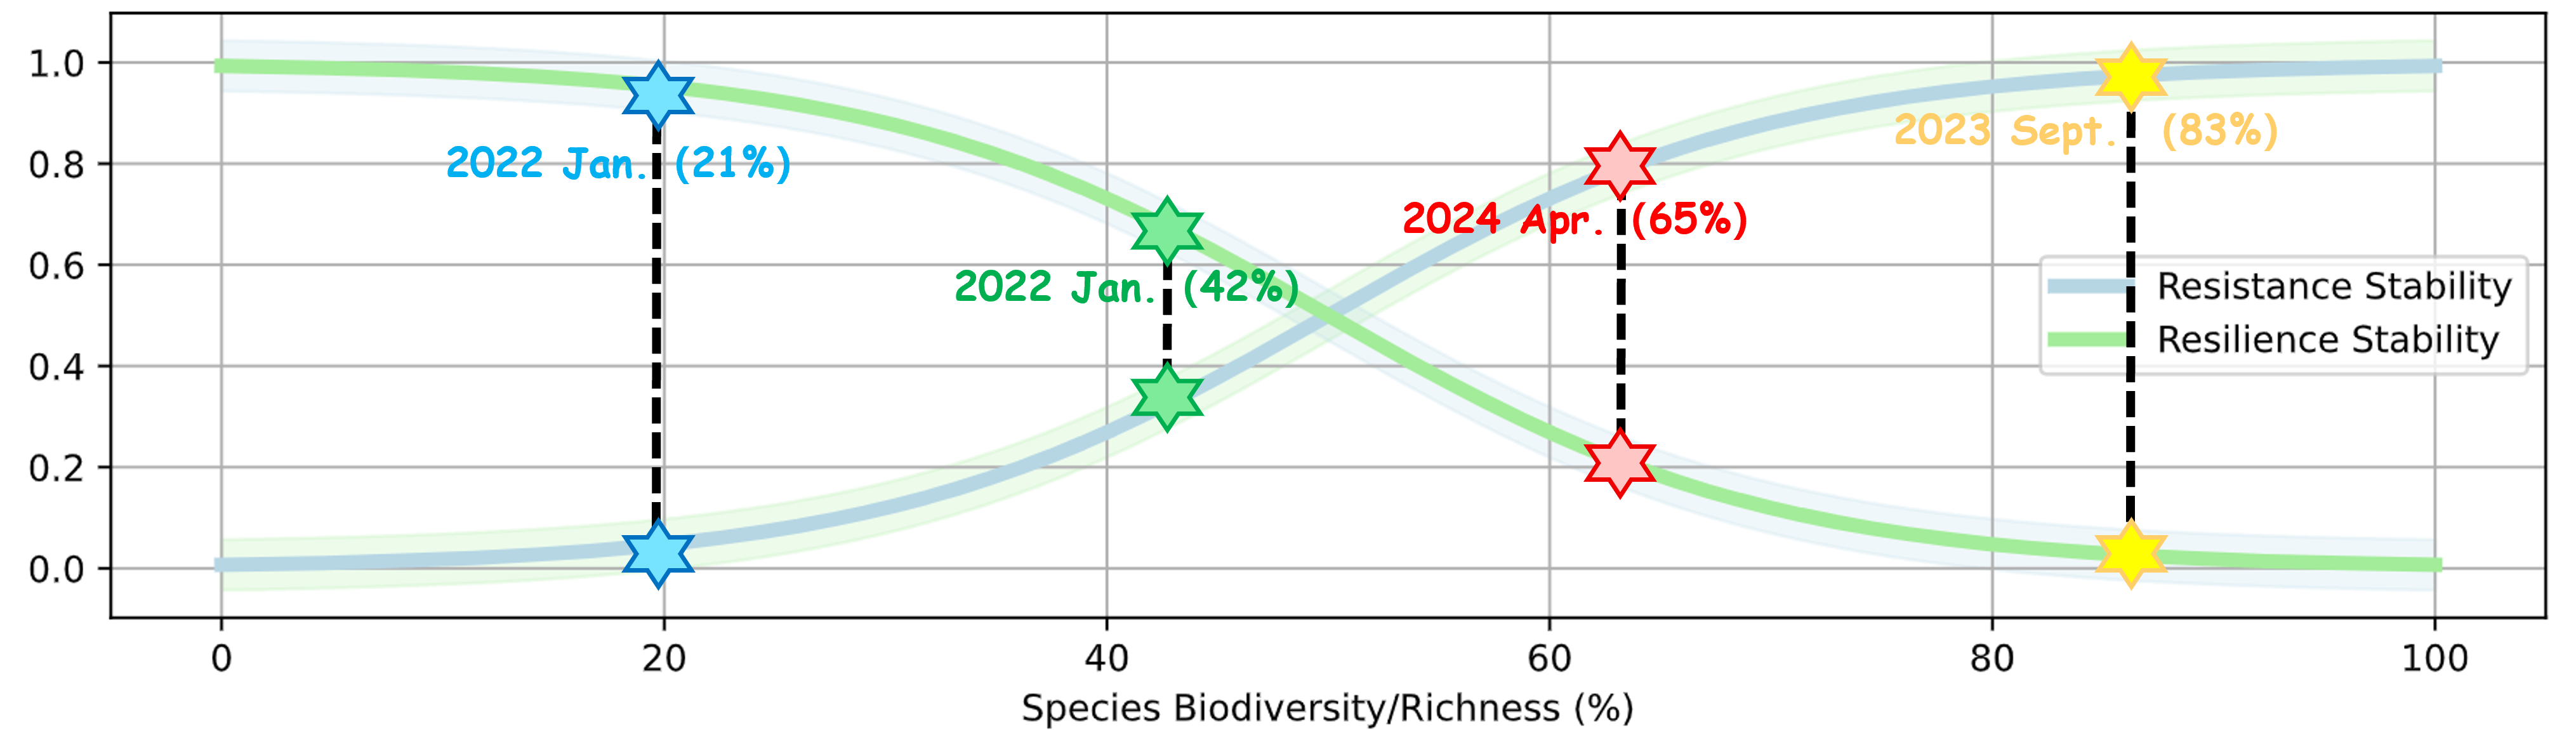
\includegraphics[width=0.8\textwidth]{./figures/resistance(task3).png}
	\caption{$RTS$ and $RLS$ when herbicide is removed. Datas are extracted from \cite{5}}
	\label{resistance}
\end{figure}

Similar to the stability analysis conducted in section 5.2, let footnote $IH$ stand for ``Including Herbicide'' and $EH$ for ``Excluding Herbicide'', from figure \ref{sbq} and \ref{resistance} we have:$$
\begin{cases}
	RTS_{EH}>RTS_{IH} \\
	RLS_{EH}<RLS_{IH}
\end{cases}\xrightarrow{ }\begin{cases}
	F_{EH}>F_{IH} \\
	(t_1-t_0)_{EH}<(t_1-t_0)_{IH}
\end{cases}\xrightarrow{ }TES_{EH}<TES_{IH}
\xrightarrow{ }Stability_{EH}>Stability_{IH}
$$

Therefore, considering the short term analysis where \textbf{the competitive impacts of weeds against crops are dismissed}, we reach to the conclusion that: When herbicide is removed, the ecosystem will become more stable. The deeper mechanism can be explained from two perspectives. On the one hand, removal of herbicide and other chemicals reduce $LSR$ by nourishing consumers and predators in food web (section 6.1.1), which in turn contributes to a higher biodiversity and system stability; On the other hand, removal of herbicide increases resistance stability and decreases resilience stability (section 6.2.2), which leads to an elevation in overall ecosystem stability. \textbf{However, the balance is doomed to break considering the drastic increase in weeds, powerful competitors against crops for nutrients.}

\subsection{Incorporation of Bats---A Long Term Solution}
\hspace{1.5em}In this section, we solve the ``weeds problems'' which inevitably destroy the ecological balance by introducing bats as the biological controlling methodology. Through integrating the Generalized Pascal's Triangle and convolution kernels, we manage to quantify and visualize the beneficial effects that bats bring to agricultural system and the interactions between bats, plants and predators. A similar species (Grass Snake) is found by rebuilding the kernels, whose impacts to the surrounding environments can be revealed in kernel's receptive fields.

\subsubsection{Bats' Interactions with Ecosystem}
\hspace{1.5em}\textbf{Review of core concepts.} Convolution kernel reveals the dynamic interactions between certain subjects and its surrounding environments, particularly when the effects of selected subject are required to be evaluated. 
For instance, let $K$ be the kernel with a receptive field of $3\times 3$, $I$ be the $10\times 10$ input convolution area, then we have equation \eqref{juanji}, where $i,j$ represent line and column index of output signal, and $m,n$ the counterparts of convolution kernel.  
\begin{equation}
	K=\begin{bmatrix}
	K_{11} & K_{12} & K_{13} \\
	K_{21} & K_{22} & K_{23} \\
	K_{31} & K_{32} & K_{33} 
\end{bmatrix},\ I=\begin{bmatrix}
	I_{11} & I_{12} & \dots & I_{19} \\
	I_{21} & I_{22} & \dots & I_{29} \\
	\vdots & \vdots & 		& \vdots \\
	I_{91} & I_{92} & \dots & I_{99} \\
\end{bmatrix},\ O=\sum_{m=1}^{3}\sum_{n=1}^{3}K_{mn}\cdot I_{i+m-1,j+n-1}
\label{juanji}
\end{equation}


Generalized Pascal's Triangle is proposed in section 5.1, where each value stands for the normalized ratio of total species richness.

\textbf{Model Establishment. }Considering that bats play a complicated role in food webs, we design three ``Bat Kernels'' respectively for insect layer, plant layer and predator layer. These layers represent biomass of respective creatures, calculated in the following fashion  where coefficients are extracted from figure \ref{chemics}.
\begin{equation}
	\begin{cases}
Plant\ Layer = 0.864\times Total\ richness, \\ Insect\ Layer = 0.071\times Total\ Richness, \\ Predator\ Layer = 0.065\times  Total\ Richness.
	\end{cases}\label{ca}
\end{equation}

Since bats are modeled as insectivores that control pest populations and flourish plants, convolution kernels are designed as figure \ref{kernel}. Each value in kernel is proposed through rigorous evaluations. Let $\omega_{ij}(i,j\in{1,2,3})$ stands for the numbers in kernels, we define $\omega_{ij}>1$ as ``bats support the objects' reproduction'' while $\omega_{ij}<1$ the opposite. Additionally, $\omega_{ij}\propto supporting\ extent$. Obviously, bats stimulate plant reproduction by clearing pests and certain competitor species, so $\omega_{ij}$ in plant layer kernel all surpass 1. In section 4.1, our EEIM model describes bats as predators to insects while competitors against other herbivores. Therefore, the majority of $\omega_{ij}$ in insect layer kernel and predator counterparts are less than 1, since the existence of bats worsens their living conditions.
Then the layers before introducing bat kernels are calculated based on equation \eqref{ca}, as is demonstrated in figure \ref{layers}. Finally, we convolve the kernels on corresponding layers (equation \eqref{juanji}, figure \ref{haokun}).
\begin{figure}[h]
	\centering
	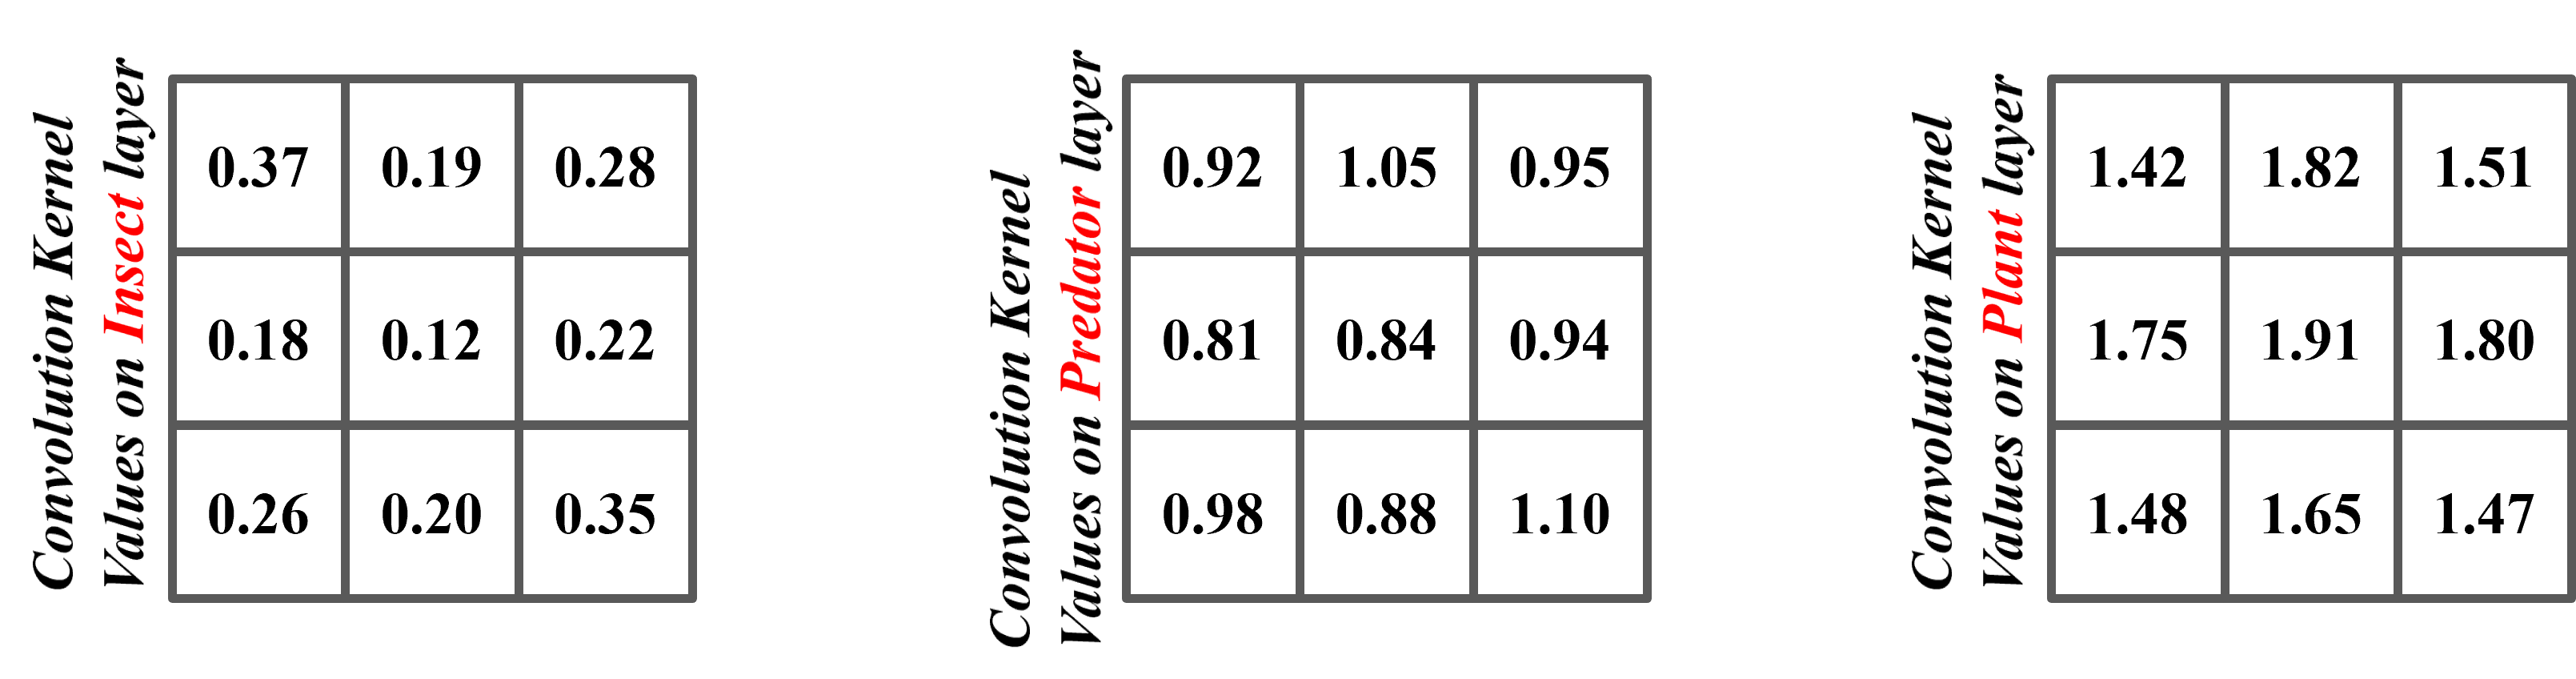
\includegraphics[width=0.8\textwidth,trim=0cm 0.3cm 0cm 0.5cm,clip]{./figures/kernel(task3).png}
	\caption{Three $3\times3$ convolution kernels for different layers, namely \textbf{Bats Kernels.}}
	\label{kernel}
\end{figure}
\begin{figure}[h]
	\centering
	\begin{subfigure}{0.22\textwidth}
		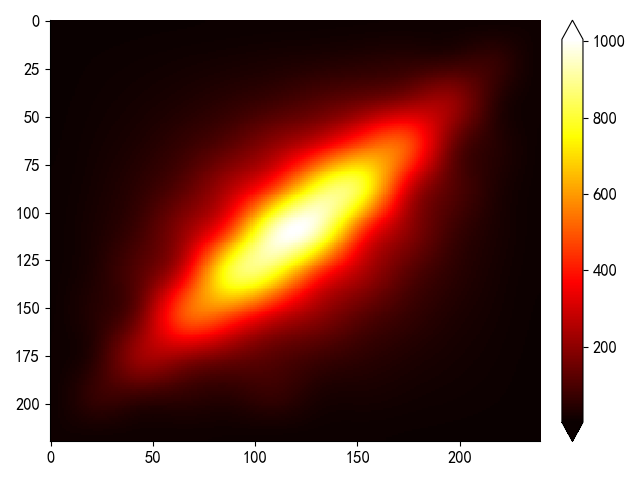
\includegraphics[width=\textwidth,trim=0cm 0.3cm 0cm 0.5cm,clip]{./figures/primitive(task3).png}
		\caption{Total Richness}
	\end{subfigure}
	\begin{subfigure}{0.22\textwidth}
		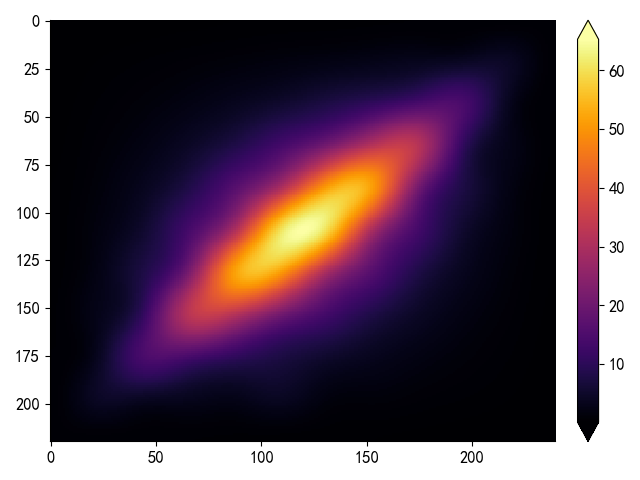
\includegraphics[width=\textwidth,trim=0cm 0.3cm 0cm 0.5cm,clip]{./figures/predator(task3).png}
		\caption{Predator Layer}
	\end{subfigure}
	\begin{subfigure}{0.22\textwidth}
		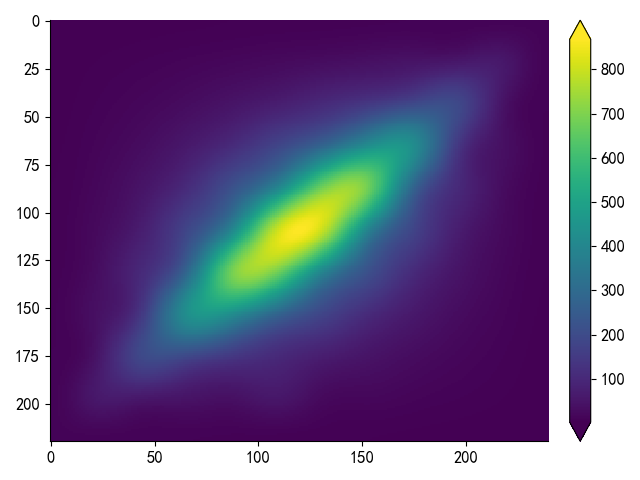
\includegraphics[width=\textwidth,trim=0cm 0.3cm 0cm 0.5cm,clip]{./figures/plant(task3).png}
		\caption{Plant Layer}
	\end{subfigure}
	\begin{subfigure}{0.22\textwidth}
		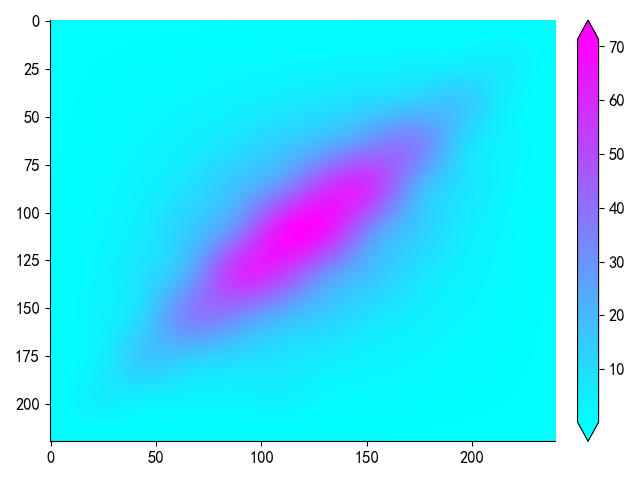
\includegraphics[width=\textwidth,trim=0cm 0.3cm 0cm 0.5cm,clip]{./figures/insect(task3).png}
		\caption{Insect Layer.}
	\end{subfigure}
	\caption{Calculation of Layers before bat kernel convolution.}
	\label{layers}
\end{figure}

\begin{figure}[h]
	\centering
	\begin{adjustwidth}{-0.115\textwidth}{}
			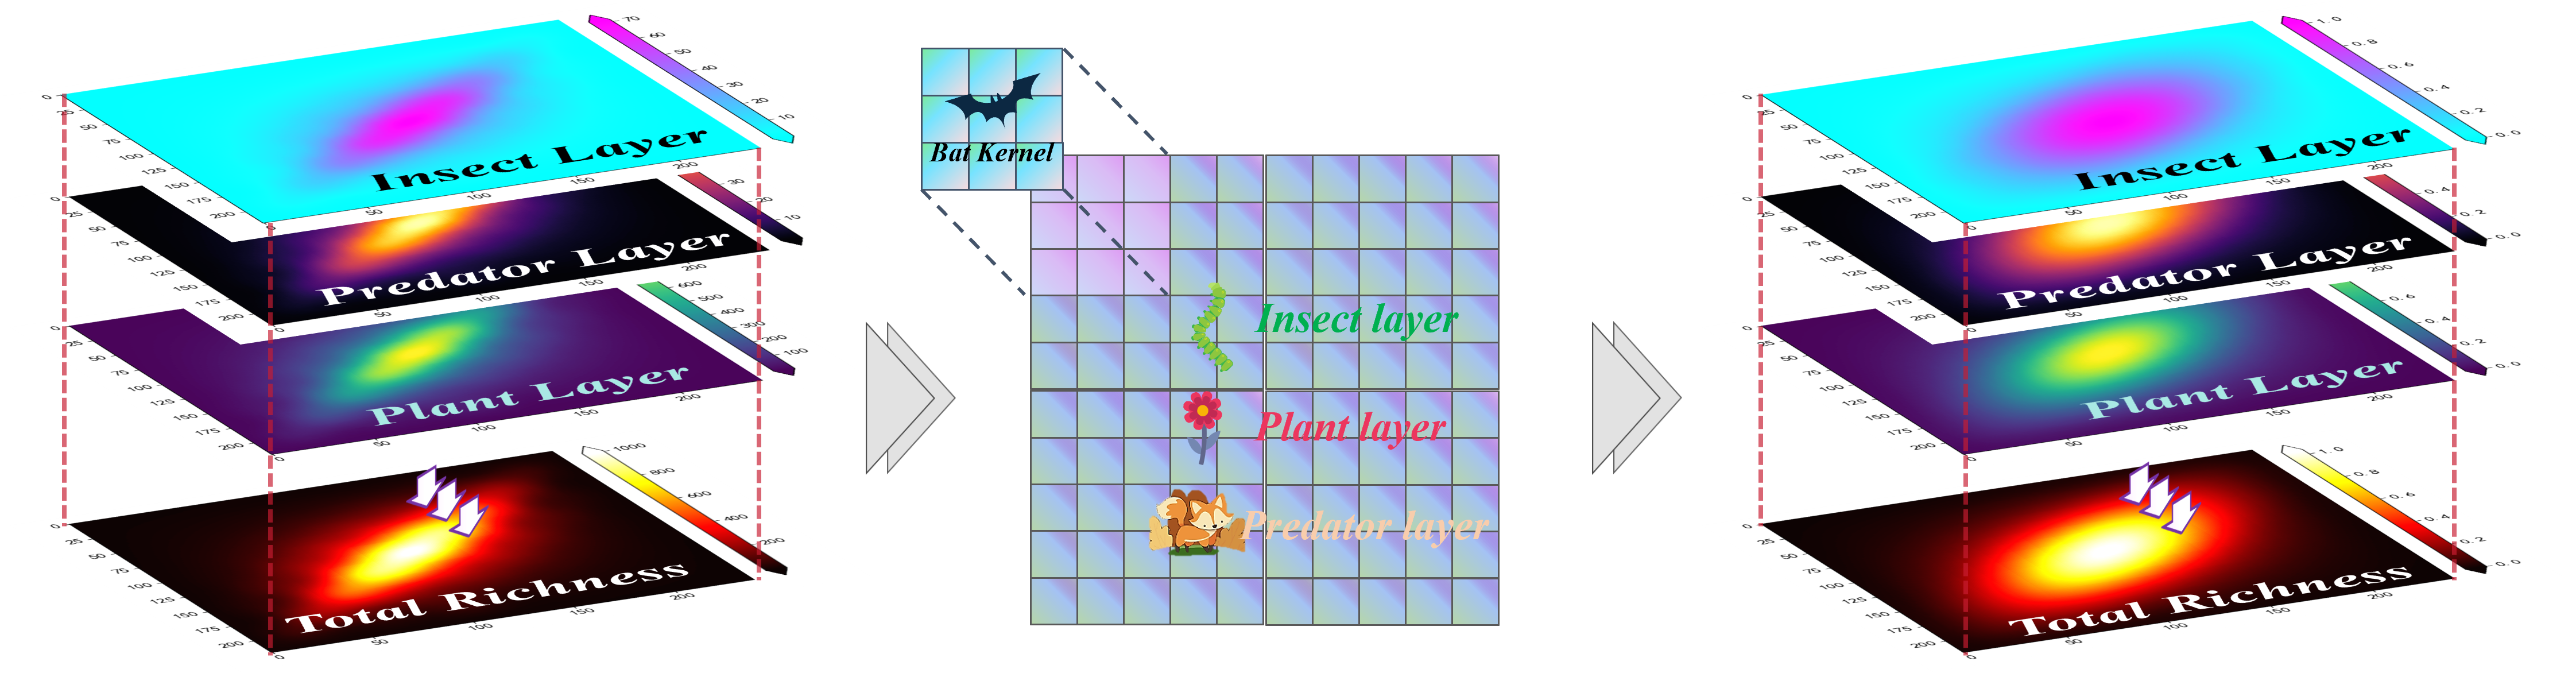
\includegraphics[width=1.2\textwidth]{./figures/convolve(task3).png}
	\end{adjustwidth}
	\caption{Bat kernel convolution on different layers and the integration of corresponding layers.}
	\label{haokun}
\end{figure}
\textbf{Explanations on Bats' Interaction with other creatures. }Take pests as the example. From figure \ref{haokun} it can be observed that pests and insects become more evenly distributed after the introduction of bats, which can be simulated by figure \ref{moni}.
\begin{figure}[h]
	\centering
	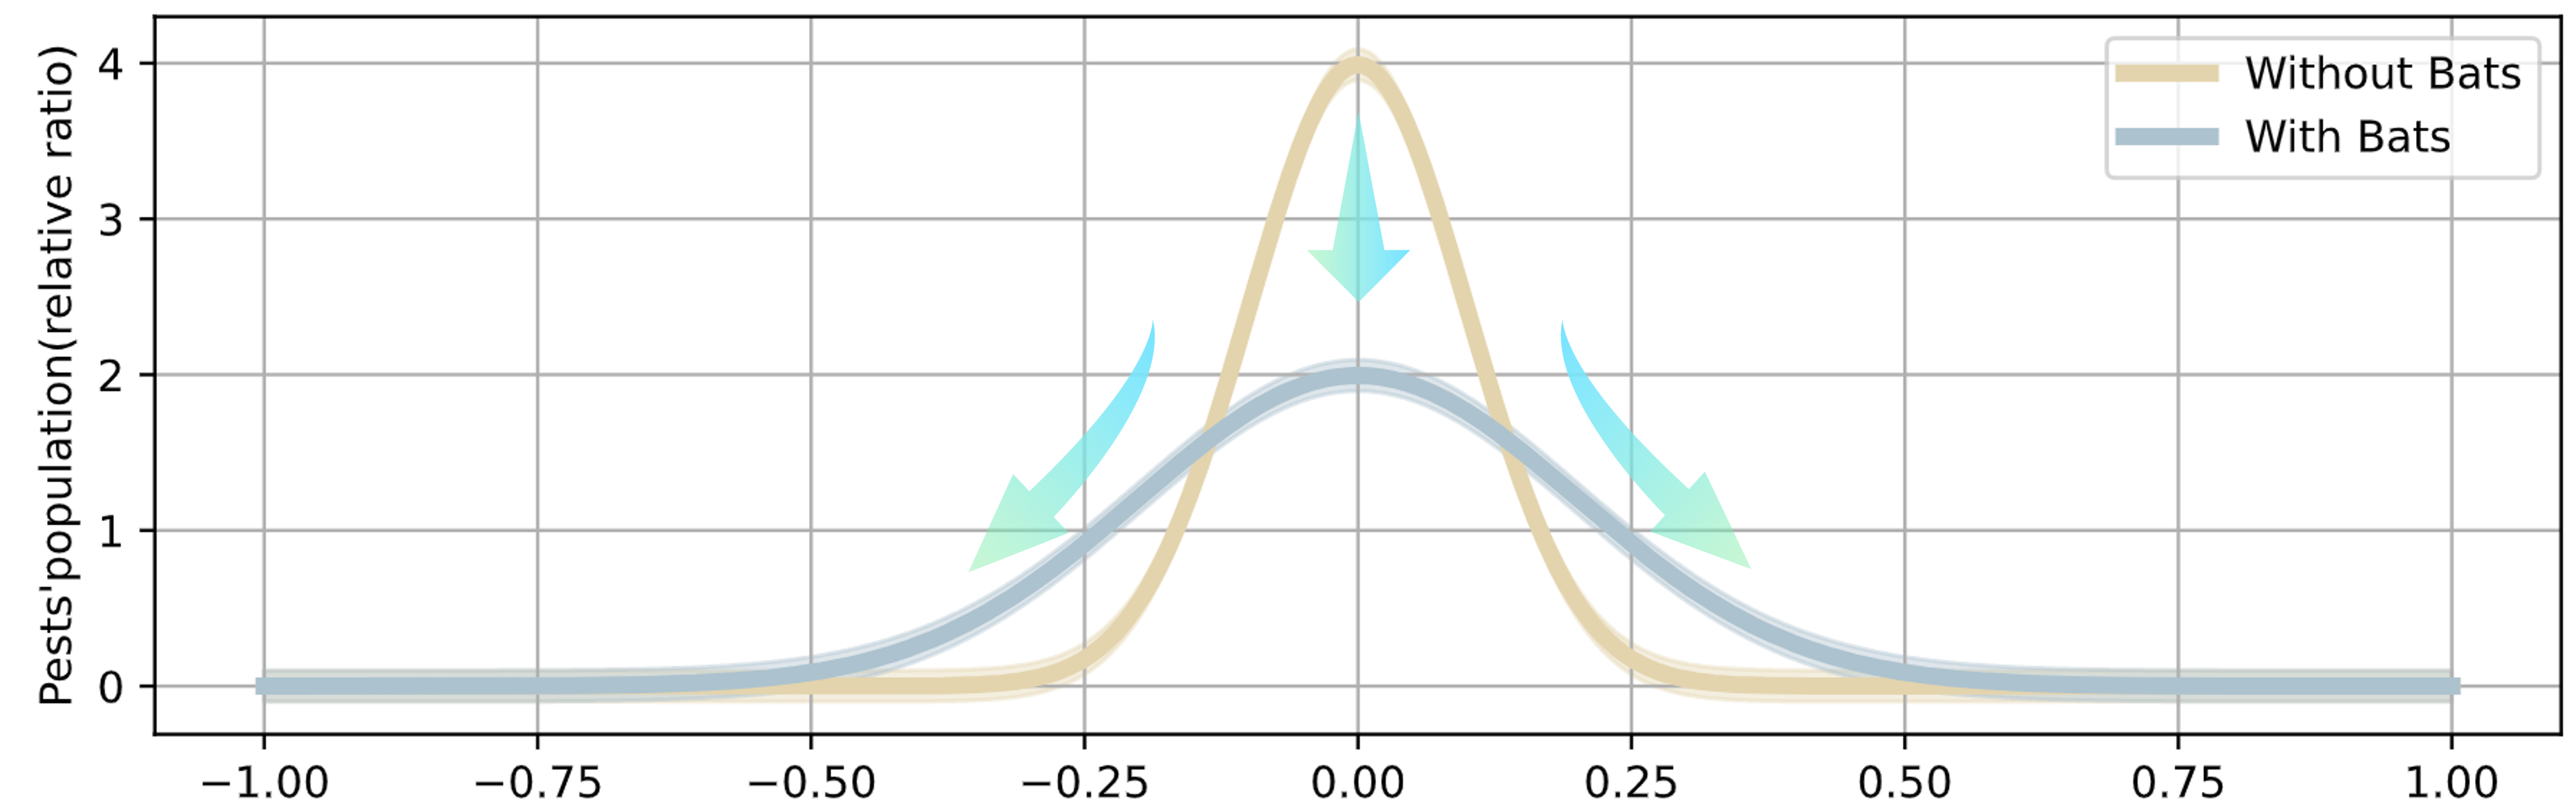
\includegraphics[width=0.82\textwidth]{./figures/Insects_expl(task 3).png}
	\caption{With and without bats considering geographical distribution of pests.}
	\label{moni}
\end{figure}
Before bats appear, pests and insects mainly survive in the central regions where crops flourish and nutrients are more than sufficient. The introduction of bats, however, turns the tables. Not only does the maximum population of pests deteriorate but they are also compelled to move into marginalized areas to escape the bats, leading to a evenly separated distribution that roughly satisfies $\mathcal{N}(0,0.2)$. Such phenomenon is also observed in figure \ref{haokun}, where the brightest areas of heat-map enlarges. Analysis alike could be conducted on predators and plants, culminating in similar conclusions which align with the results illustrated in figure \ref{haokun}.

\subsubsection{The Ecosystem Stability Outcome}
\hspace{2em}Although a prosperous biodiversity is gladly expected in mature agricultural ecosystems and we have analyzed that bats definitely contributes to such wishes, it does not, however, necessarily lead to the stability.

In section 5.2 we introduce the Ecosystem Stability Model which comprises three sub-variables: $RTS$, $RLS$ and $TES$. Considering the primary goal of agricultural ecosystems is to harvest, neither $RTS>>RLS$ or $RTS<<RLS$ is what we expect. For instance, when $RTS\to0$, the ecosystem is too weak to stand any disturbance (e.g., harsh winters); when $RLS\to0$, the ecosystem suffers severe economic losses when extreme weather events attack since the system is too complicated to recover. In figure \ref{resistance}, we correlate $RLS$ and $RTS$ with species richness, meaning that in order to maintain a stable agricultural ecosystem, species richness have to be confined within a finite range. 
\begin{figure}[h]
	\centering
	\begin{subfigure}[b]{0.3\textwidth}
		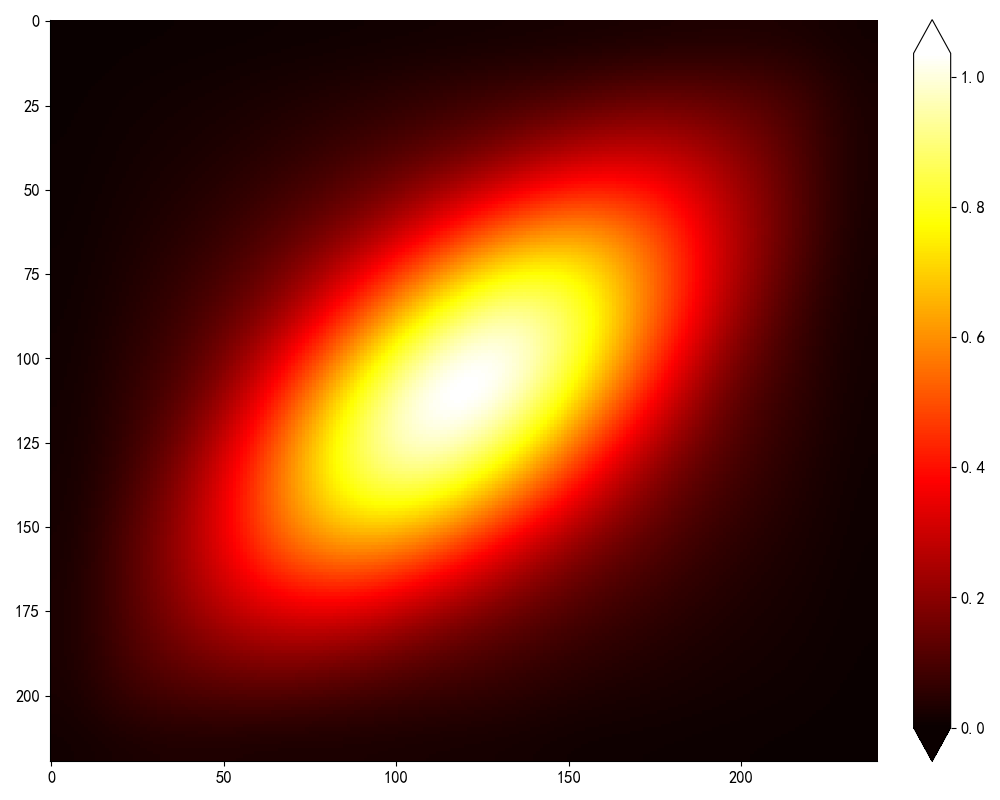
\includegraphics[width=\textwidth]{./figures/withbats(task3).png}
		\caption{Species Richness distribution.}
	\end{subfigure}
	\begin{subfigure}[b]{0.35\textwidth}
		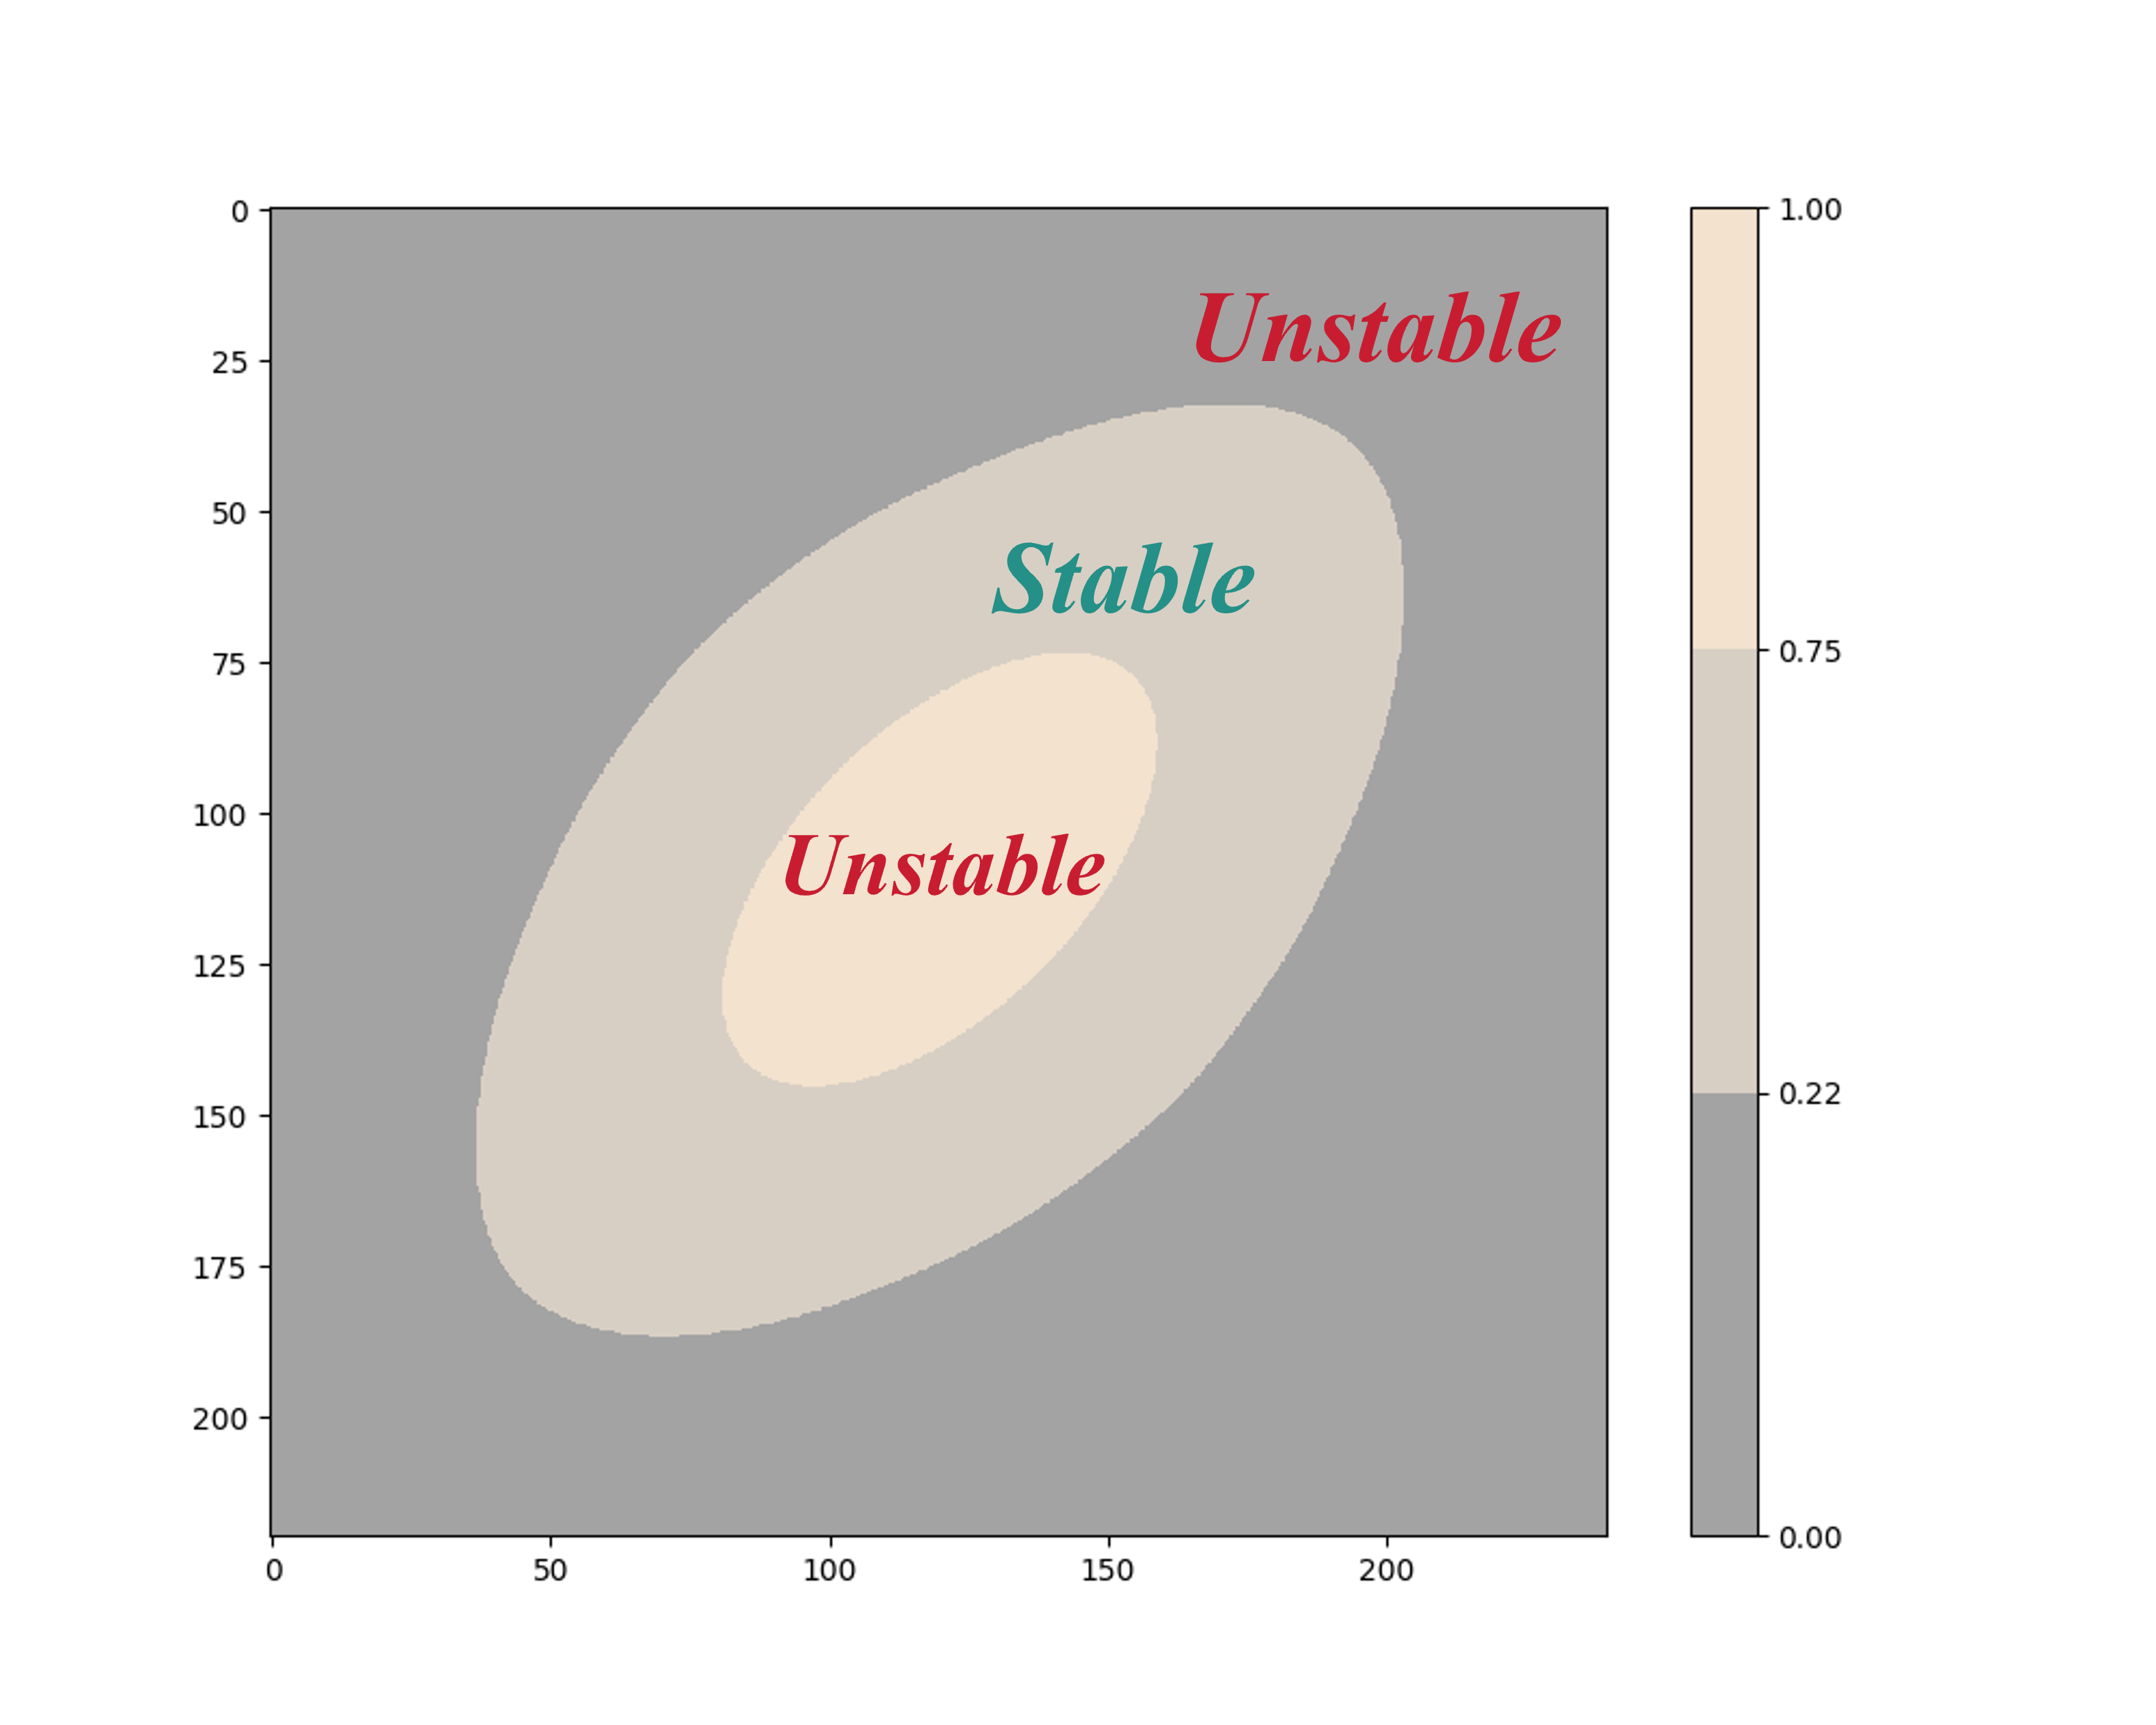
\includegraphics[width=\textwidth,trim=0cm 1.4cm 0cm 0cm, clip]{./figures/stability_interval(task3).png}
		\caption{Categories of stability}
	\end{subfigure}
	\caption{Ecosystem stability interval: $Species\ Richness\in[22\%,75\%]$ }
	\label{tong}
\end{figure}
Referring to figure \ref{tong} and \ref{resistance}, we acquire equation \eqref{cheng}, where $Species\ Richness$ corresponds to the $y$-coordinates of figure \ref{sbq}, namely our food web model output.
\begin{equation}
	\begin{cases}
		Species\ Richness\in[22\%,75\%]\xrightarrow{}\text{\textbf{Stable}} \\
		Species\ Richness\in[0\%,22\%)\cup(75\%,100\%]\xrightarrow{}\text{\textbf{Unstable}}
	\end{cases}
	\label{cheng}
\end{equation}

In summary, introducing bats does solve the ``weeds problem''. However, even though bats' positive interactions with plants, predators and insects do contribute to an increased species richness which seems to stabilize the ecosystem, datas demonstrate that only when richness falls within $[22\%,75\%]$ can an agricultural ecosystem authentically evolves into a stable one.

\subsection{Grass Snake, a Species Similar to Bats}
\hspace{1.5em}Grass Snake is a species commonly found in agricultural fields, feeding on frogs, small reptiles, etc. It is a carnivorous snake with negligible predation on insects, forming a striking contrast with bats whose major food resource is insects.

As a higher-level predator in food webs, grass snake brings ecosystems back into balance by preying on harmful animals (e.g., mice). However, it indirectly controls pest population, differing from bats. Therefore, we redesign the Snake Kernels, as is illustrated in figure \ref{snake}.
\begin{figure}[h]
	\centering
	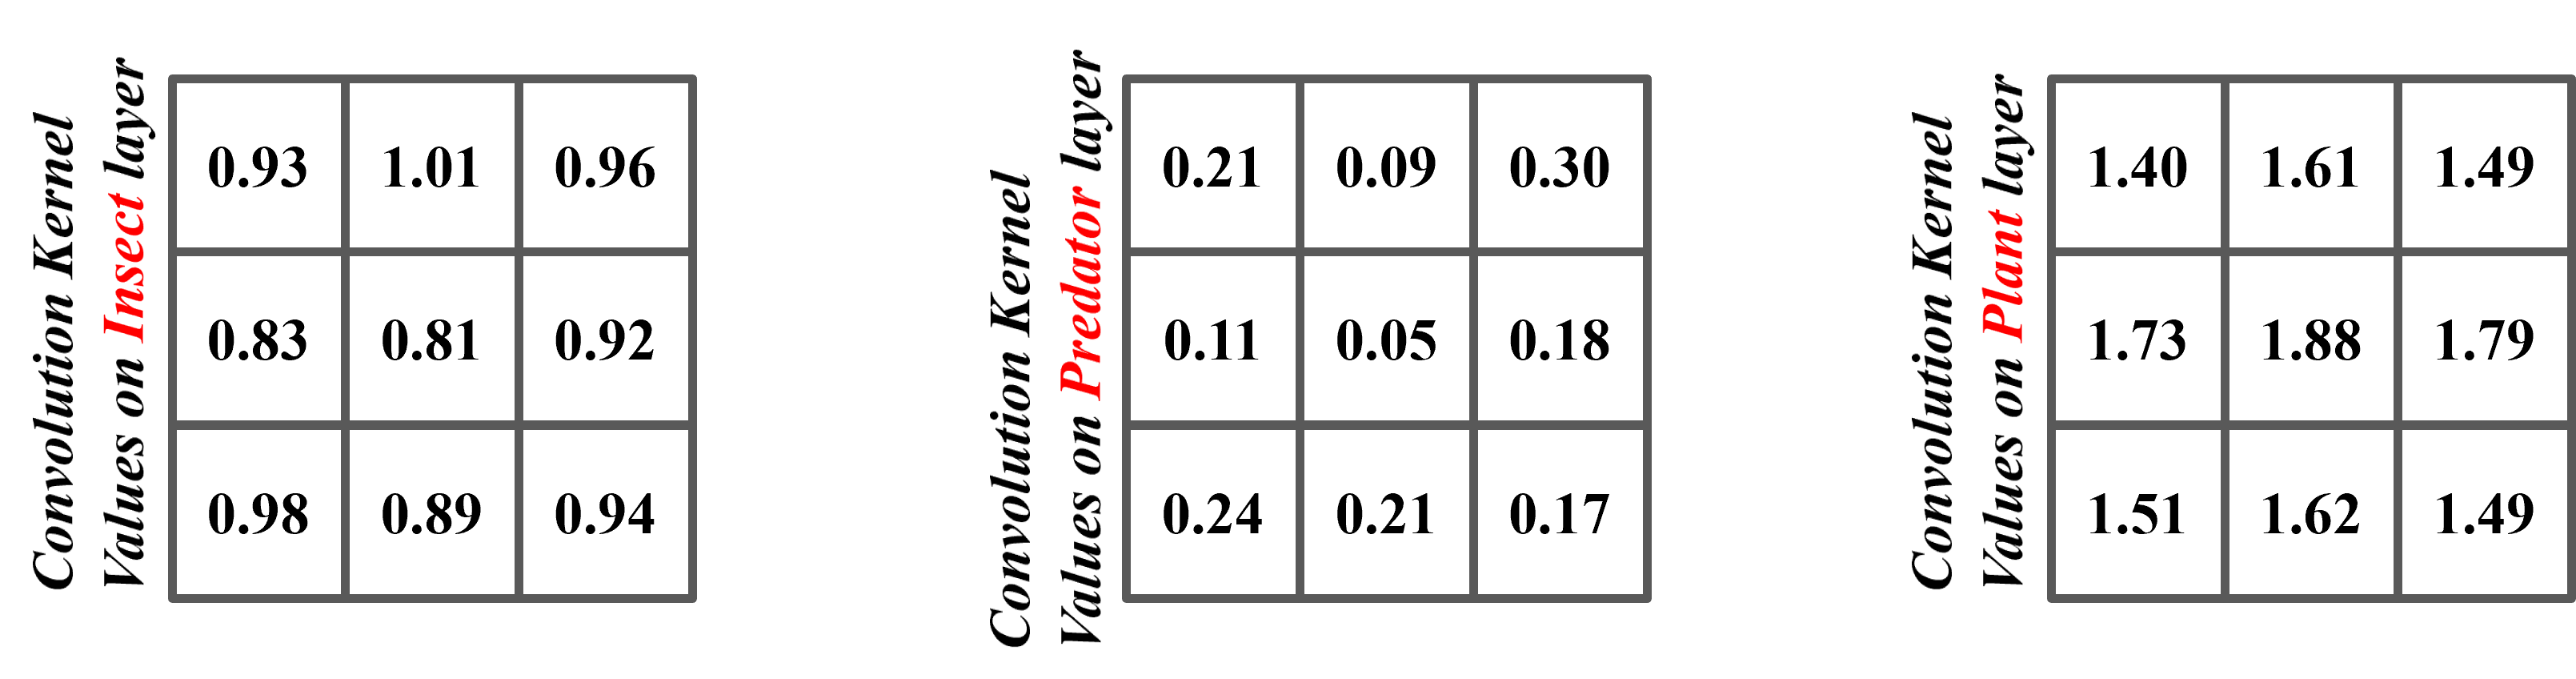
\includegraphics[width=0.9\textwidth,trim=0cm 0.3cm 0cm 0.5cm,clip]{./figures/snake_kernel(task3).png}
	\caption{Snake Kernel.}
	\label{snake}
\end{figure}
After the convolution calculations similar to figure \ref{haokun}, we further compare the differences between bat kernel results and snake kernel counterparts, which could reveal their discrepancy in essence, as is demonstrated in figure \ref{ch}. We quantificationally determine species richness by measuring the geological distance in graphs, acquiring: $c_1=c_2,\ d_1>d_2,\ b_1\approx b_2,\ a_1<a_2$. The results feature strong practical meaning.
\begin{figure}[h]
	\centering
	\begin{subfigure}{0.47\textwidth}
		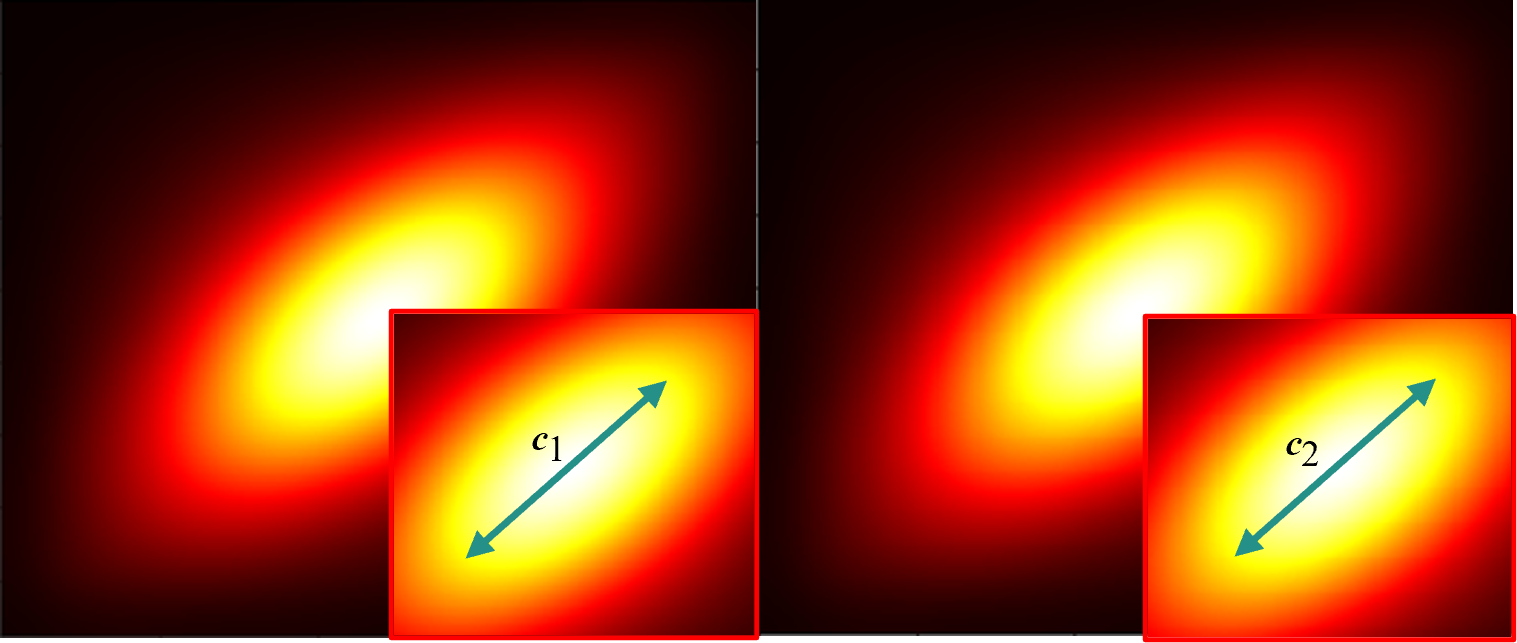
\includegraphics[width=\textwidth]{./figures/total(task3).png}
		\caption{Total Species Richness.}
	\end{subfigure}
	\begin{subfigure}{0.47\textwidth}
		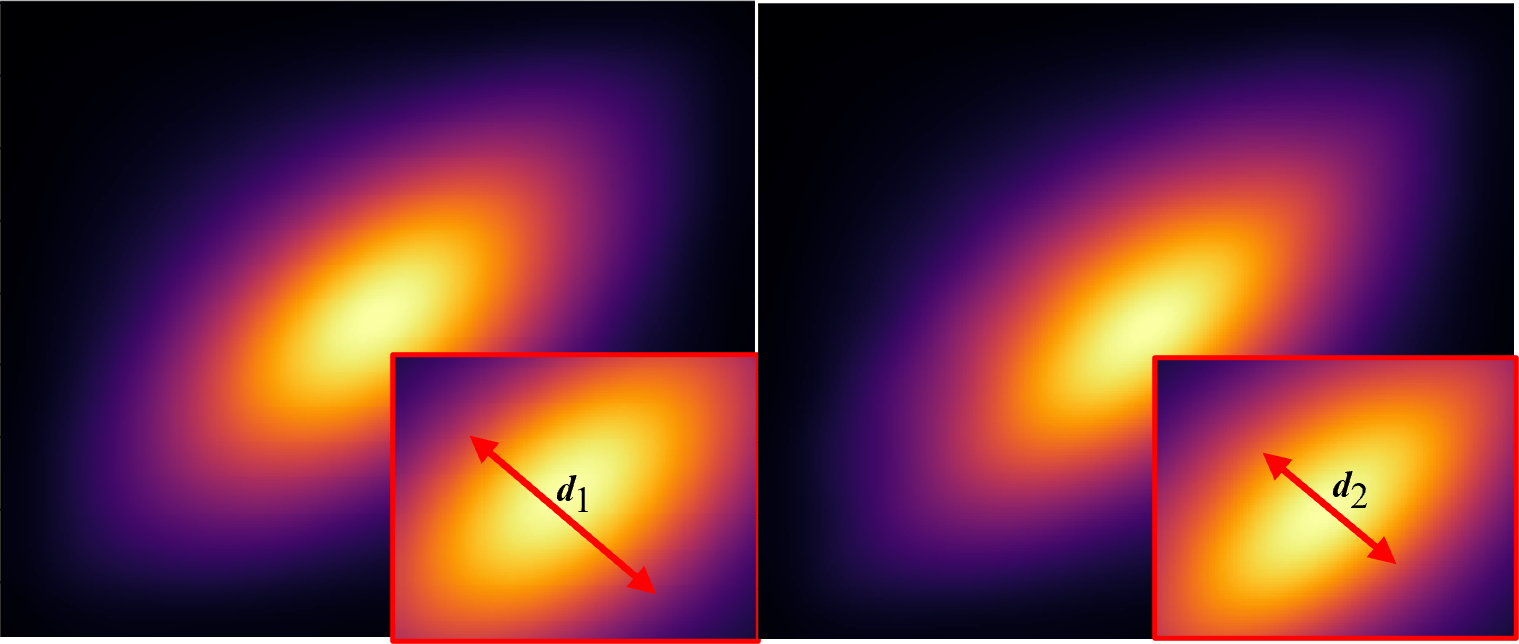
\includegraphics[width=\textwidth]{./figures/pred(task3).png}
		\caption{Predator Layer.}
		\label{pred}
	\end{subfigure}
	\begin{subfigure}{0.47\textwidth}
		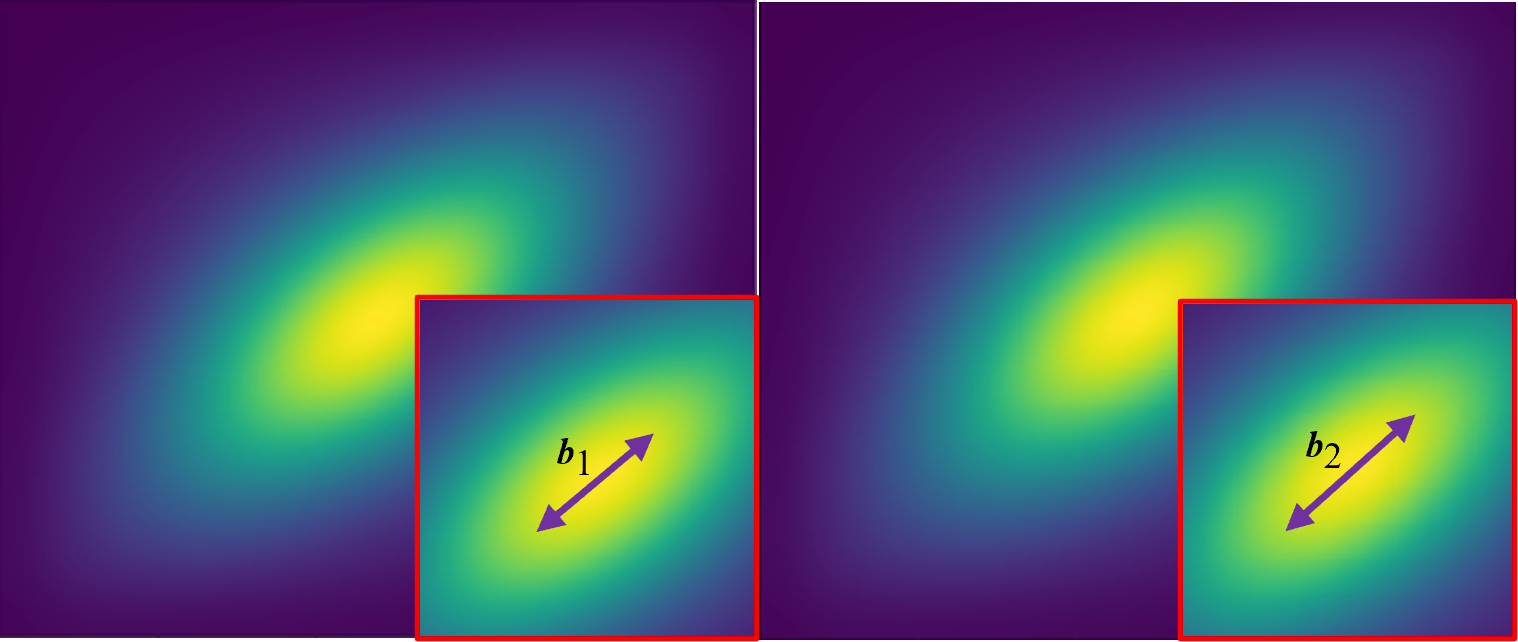
\includegraphics[width=\textwidth]{./figures/plt(task3).png}
		\caption{Plant Layer.}
		\label{zhiwu}
	\end{subfigure}
	\begin{subfigure}{0.47\textwidth}
		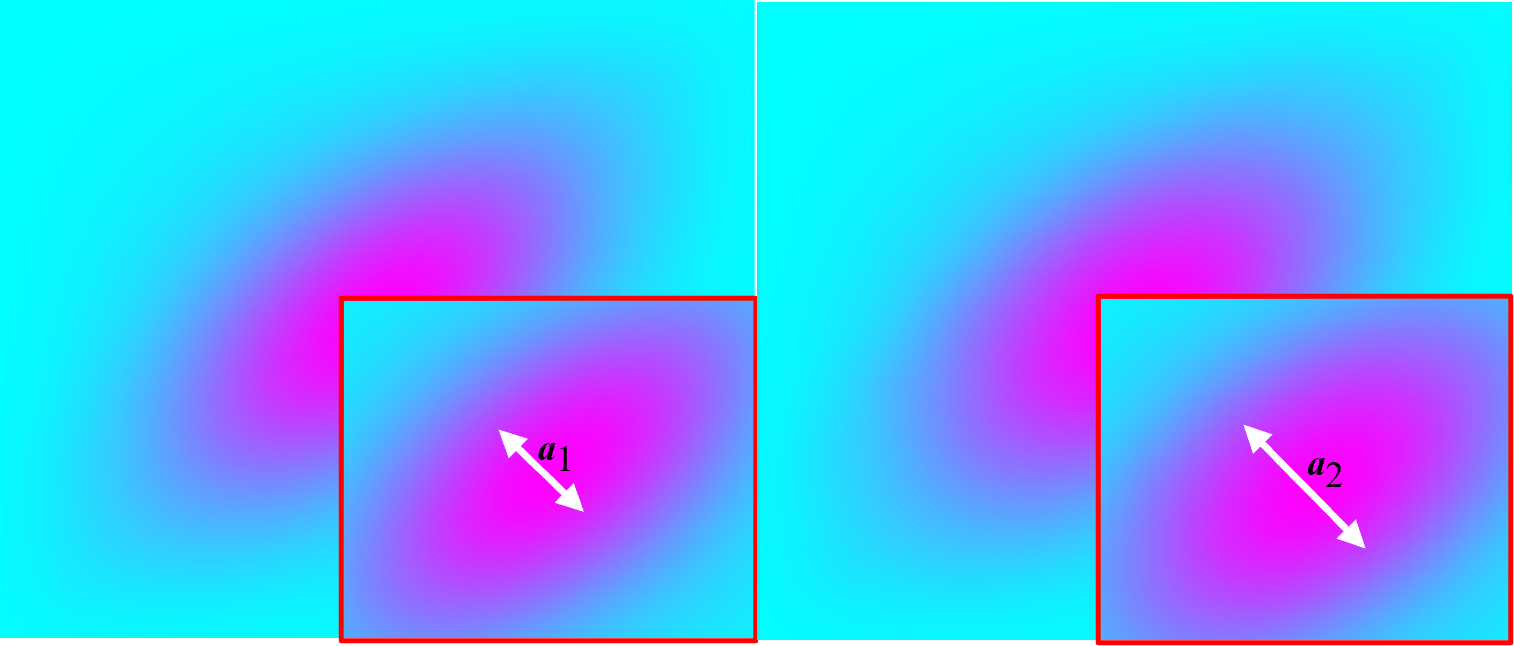
\includegraphics[width=\textwidth]{./figures/insec(task3).png}
		\caption{Insect Layer.}
		\label{chong}
	\end{subfigure}
	\caption{Comparisons between bats and snakes, where the left figures stand for snake kernels' convolution results and right ones represent bats (extracted from figure \ref{haokun}).}
	\label{ch}
\end{figure}

Firstly, from figure \ref{moni} and \ref{haokun} we reach to the conclusion that, if the animal being introduced facilitates ecosystem stability and drives the noxious creatures to marginal habitats, richness distribution becomes more even. In heat-maps such as figure \ref{tong}, the brightness area appears broader on the graph. In figure \ref{ch} from  $c_1=c_2$, we conclude that grass snakes and bats have similar impacts on ecosystem stability considering total species richness and biodiversity, while on the detailed food web components, two species differ. As a higher-level predator, grass snakes pose deeper impacts on other predators while bats don't, causing $d_1>d_2$ in figure \ref{pred}; Since both species all benefit agricultural system, the differences of their effects on plants and crops is negligible, resulting in $b_1\approx b_2$ in figure \ref{zhiwu}; As for the pests and other insects, bats influence more than grass snakes since bats are lower-level predators and could directly impact insect population through preying while grass snakes cannot, culminating in $a_2>a_1$ in figure \ref{chong}. 

In summary, grass snakes could facilitate the agricultural ecosystem stability just as bats do. However, their inner mechanisms contrast significantly. Bats, as lower-level predators, directly control pest population through preying  and have negligible impacts on trophic level consumers; Grass snakes, as higher-level predators, directly impact other consumers and indirectly control the pest population generally relying on the chain-reactions of food webs. Both species have similar effects on plants and crops, since the primary goal of an agricultural system is to harvest.

\section{Implications of Organic Farming}
\hspace{1.5em}Organic agriculture is a sustainable system based on ecological principles, emphasizing natural cycles and biodiversity. It avoids synthetic chemicals and employs biological control to enhance soil fertility and boost yields. This approach maintains ecosystem health while producing nutritious foods.

Due to the low nutrient content in soil and low biodiversity indices in the initial stages of agricultural ecosystem development, we have determined through reviews (\cite{8}) that it is not advisable to adopt organic farming practices during primary forest-to-farm stages. Therefore, we focus on mature agricultural ecosystems.

To analyze the impact of various measures compliant with organic farming standards on the ecosystem, the Multi-objective Optimization Model is employed. We decompose the major objectives into three  sub-ones: biological health, ecosystem stability, and economic efficiency. This allows us to build an objective optimization function. Simulated Annealing algorithm is then utilized to derive effective solutions for these sub-objectives, thereby identifying the most ideal goal achievable for agricultural ecosystems following the adoption of organic farming practices.

Therefore, a detailed analysis of how organic farming practices influence agricultural ecosystems is conducted. Our study clarifies the mechanisms of which practice of transforming farmlands could achieve a win-win solution in both ecological and economic situations.

\subsection{The Multi-objective Optimization Model}
\hspace{2em}Based on the principles of multi-objective programming models, we first analyze and determine the priorities of the aforementioned sub-objectives. For the biological health $P_1$, it encompasses the biomasses $x_i(i = 1,2,3,4)$ of various species, including pests, crops, etc. The ecosystem stability  $P_2$ is jointly represented by $RTS$ and $RLS$ of ecosystems. The economic efficiency $P_3$ is composed of crop revenue $x_5$ and total costs $x_6$ associated with planting and managing the farmland. We ultimately determine the priority sequence as $P_1 > P_3 > P_2$ referring to existing researches.
\begin{equation}
    MIN\;y=P_1d_1^-+P_2d_2^-+P_3d_3^-
\end{equation}

Datas from region $Q$ (section 4.1.3) are adopted and we introduce positive deviation variables $d_i^+$ and negative counterparts $d_i^-$ for the formulation of goal programming function.

To this end we have equation \eqref{opt} where $H$ represents the stability of the ecosystem prior to implementation of organic farming practices, $M$ denotes the previous agricultural yields from farmland, and $S_{Q}$ indicates the area of region $Q$.

In the multi-objective planning function $y$, all negative deviations from constraints should be measured and minimized to ensure that the objectives for implementing organic farming practices are achieved.

Among the constraints, it is evident that biomass of all species should not exceed the maximum environmental carrying capacity of agricultural ecosystem. Considering the beneficial practice in organic agriculture of introducing natural predators of pests, we assert that biomass of crops should not be less than the biomass of pests.
\begin{equation}
\text{s.t.} \\
  \begin{cases}
   x_1 + x_2 + x_3 + x_4 \leq K = 10^{k_0} \sum_{i=pro}B_i\\
   x_2 + x_3 + x_4 - x_1 + d_1^- - d_1^+ = 0 \\
   \int_{t_1}^{t_2} \sum\limits_{i=1}^{4} \left| g_1(t) - g_2(t) \right| \, dt + d_2^- - d_2^+ = 1.2H \\
   x_5 - x_6 + d_3^- - d_3^+ = M\\
   x_5 = 0.259x_2\times S_{Q} \\
   x_6 =S_{Q}\times (0.105x_2+ 0.119x_4)\\
   x_i,d_m^-,d_m^+\geq 0  (i=1,2,3,4,5,6;m=1,2,3)
\end{cases}  
\label{opt}
\end{equation}

Furthermore, through integrating the calculation methods for assessing stability of a mature farmland as outlined in section 5, the ecosystem's stability over a specified time period must be no less than 1.2 times its previous stability. 

To calculate the costs and benefits of agricultural production, we link crop yield with price by combining the definition of biomass, the annual average selling price of crops in region $Q$, and the cost of seeds. In particular, we account for the costs associated with soil fertility improvements after implementation of organic farming practices. This consideration leads to adjustments in the cost-constrained formula to better reflect real-world conditions. Then, profit constraints are imposed to ensure financial viability and sustainability.

Finally,we utilize the Simulated Annealing Algorithm for solving the problem, setting the maximum number of iterations to 3000 to ensure the validity and effectiveness of the obtained solution.

\begin{figure}[h]
    \centering
    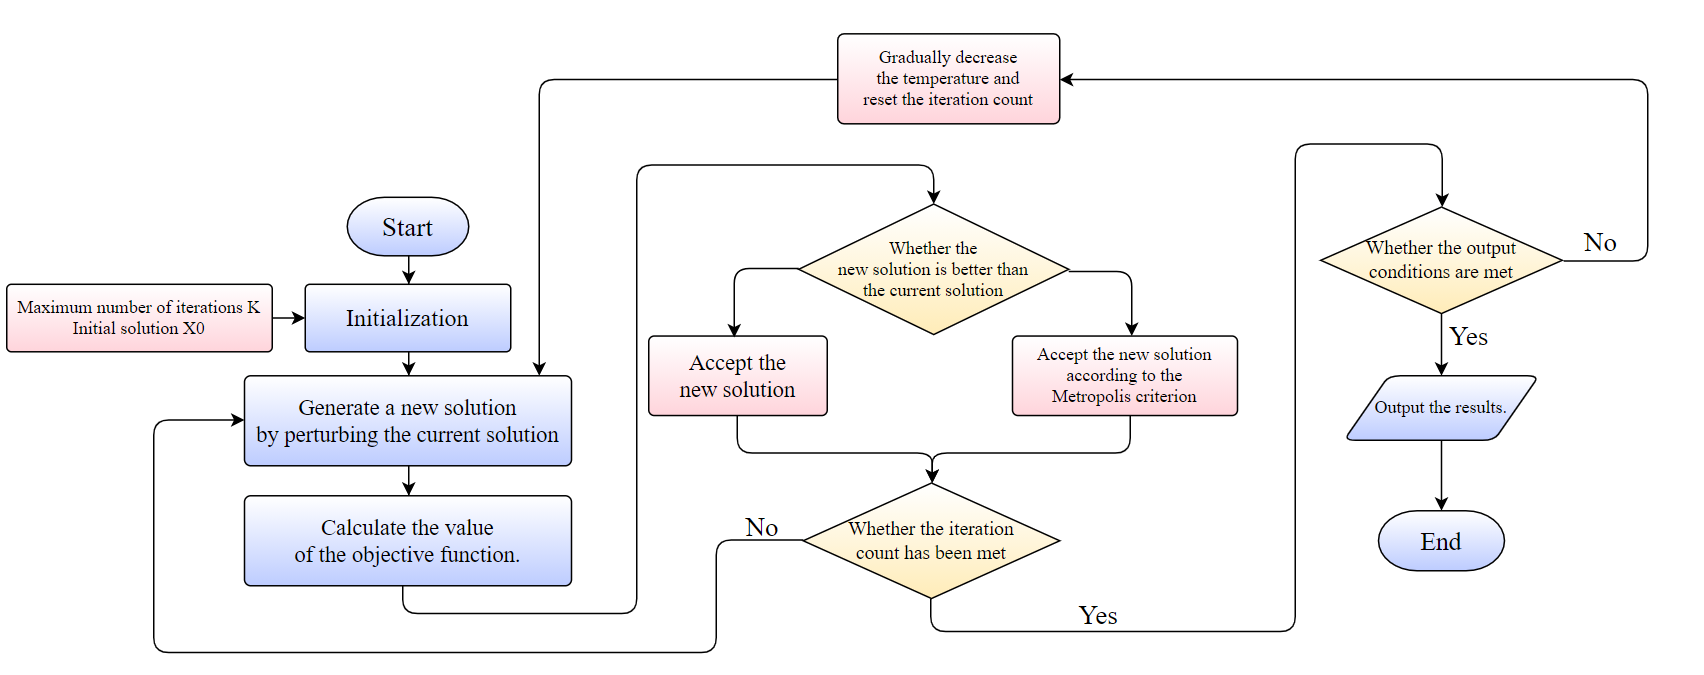
\includegraphics[width=0.8\textwidth]{./figures/SA.png}
    \caption{Flowchart of the Simulated Annealing Algorithm}
    \label{fig:my_label}
\end{figure}

\subsection{Detailed Analysis}
\hspace{2em}When farmers engage in organic farming, the agricultural ecosystem will change significantly. This section explains it from diverse dimensions.

\textbf{Pests control}. After controlling the utilization of chemicals, we recommend farmers to plant crops that are conductive to pests' enemies'  reproduction, or employ organic products to decrease the mating rate of pests. Though their population will rise temporarily, it  soon drops significantly (figure \ref{pest}), because even $r$ gets larger, secondary predators will limit their reproduction:
\begin{equation}
    \frac{dB_{pest}}{dt}=r'_{pest}B_{pest}(1-\frac{B_{pest}}{K_{pest}})+\sum_{i=pro} a_{pes-i}B_{pest}B_k-\sum_{j=pre} \beta_{j-pes}B_{pest}B_j-p
\end{equation}
where $r'_{pest}>r_{pest}$  but $j$ is larger, which means an increase in enemies' population, let alone $p>0$.

\begin{figure}[h]
    \centering
    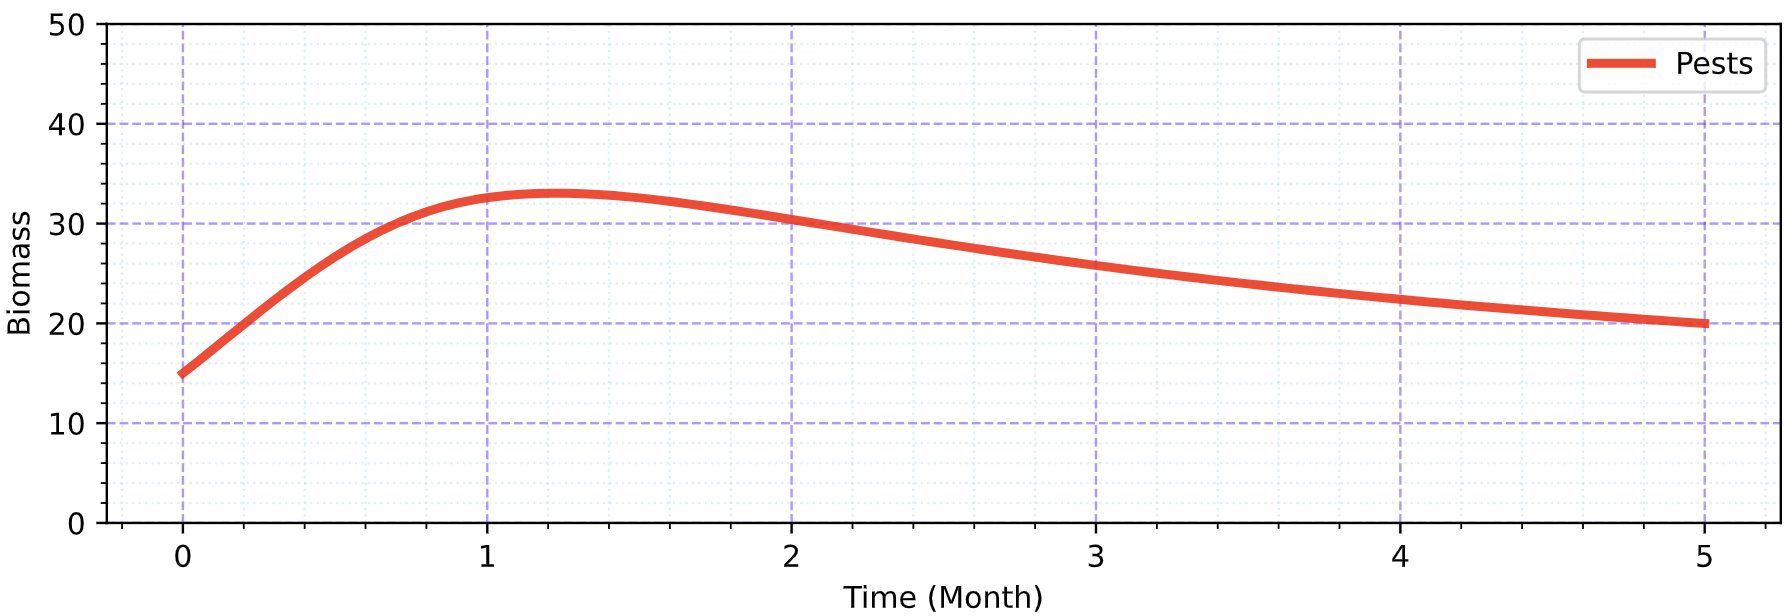
\includegraphics[width=0.6\textwidth]{./figures/pests.png}
    \caption{Biomass of pests after organic farming}
    \label{pest}
\end{figure}

\textbf{Crop health}. Chemicals are double-edged swords, on the one hand, they promote yields and defend crops from pests; on the other hand, they lead to reduction in crops nutrition. After the removal of chemicals, the plants’ health alters in the following fashion, where $N$ is nutrition and $D$ is damage caused by pests:
\begin{equation}
    \Delta H=\Delta N -\Delta D
\end{equation}

\textbf{Plant reproduction}. Plants include crops and weeds. In the absence of chemicals, weeds would intrude upon crops. To address this issue, farmers need to manually remove weeds or apply organic mulches. It is more recommended to change the types of crops grown in a specific field each season, which can disrupts weeds’ life cycle.

\textbf{Biodiversity}. Removal of chemicals is beneficial to biodiversity, as is mentioned in section 5 and 6. Additionally, we notice that by altering what to grow in each season can also stimulate the biodiversity.

\textbf{Long-term sustainability}. Ecological cost (EC) is an important indicator for measuring the damage to ecosystems. The higher the ecological cost, the weaker the sustainability of the ecosystem. According to [6], we have:
\begin{equation}
    EC=EC_f+EC_p=EC_{f1}+EC_{f2}+EC_{f3}+EC_p
\end{equation}
where $EC_{f1}$, $EC_{f2}$, $EC_{f3}$ refer to the costs of polluting the atmosphere, water and soil with fertilizers respectively, $EC_p$ is pesticide costs. After chemicals are removed, the costs aforementioned will be weakened significantly.

\textbf{Costs effectiveness}. Practicing organic farming does not rely on chemicals($C_1$) or costly machinery($C_2$), reducing farmers' operational costs. Meanwhile, organic products often fetch better prices in the market($\Delta P_1$). Even if the initial yield is lower($\Delta P_2$), the profit per unit may be higher. Moreover, the long-term environmental benefits can offset the initial investment costs of organic farming.
\begin{equation}
    CE=\frac{P_0+\Delta P_1-\Delta P_2}{C_0-C_1-C_2}
\end{equation}















%%%%%%%%%%%%%%%%%%%%%%%%%%%%%%鲁棒性分析
\section{Sensitivity and Robustness Analysis}
\hspace{2em}\textbf{Sensitivity Analysis. }Since our EEDM model is a crucial part in the simulation of human impacts on agricultural ecosystems, we calculate the Sensitivity Coefficient for equation \eqref{primitive} and \eqref{time}, which goes as:
\begin{equation}
	Sensitivity\ Coefficient(SC\  \text{for short})=\frac{\frac{\partial LSR}{\partial t}\times t}{LSR}=\frac{(-0.02924\times t+59.17)\times t}{-0.01462\times t^2+59.17\times t-59845.89}
\end{equation}
Let $t=2025$, we have $SC=-2.851556$ and we acquire $LSR(t=2025)=27.6\%$ which indicates that $LSR$ will drop to $26.8129\%$ till year 2045. Therefore, the outputs of EEDM isn't sensitive to time. Considering the practical meaning of EEDM model, such result implicates that if no measures are deliberately taken to reduce chemical use, our ecosystems may suffer severe losses in biodiversity at an astonishing rate and the deteriorating speed isn't likely to shrink automatically.

\textbf{Robustness Analysis. }The Monte Carlo Algorithm is employed to test the robustness of our MLP neural network proposed in section 4.2. Results are illustrated in figure \ref{mt}. 
\begin{figure}[h]
	\centering
	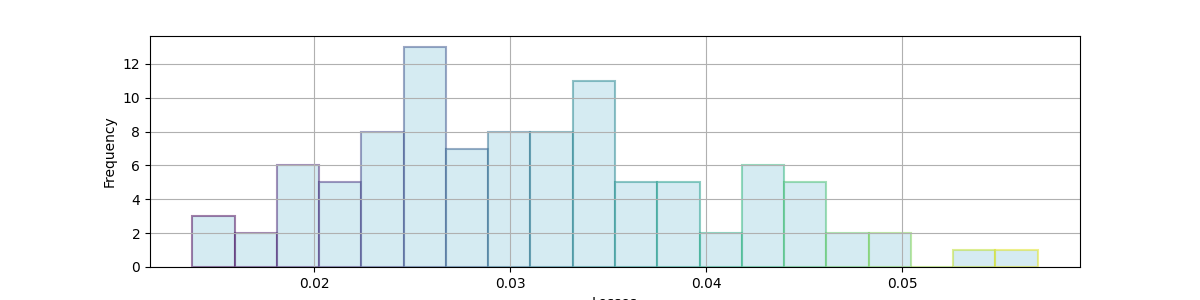
\includegraphics[width=\textwidth,trim=0cm 0.1cm 0cm 0.92cm,clip]{./figures/Monte Carlo.png}
	\caption{Results of Monte Carlo Robustness Testing.}
	\label{mt}
\end{figure}
	
From figure \ref{mt} we have $Mean\ loss=0.03123$, $Standard\ Deviation\ of\ Loss=0.00917$. Therefore we reach to the conclusion that our model converges successfully and features strong robustness and generalization ability, which as well proves the rationality of our following analysis.
	


\section{Evaluation of our Models}
\hspace{1.5em}\textbf{Strengths. }Firstly, deep-learning methods are deployed into practical use, acquiring ideal effects. Secondly, an innovative generalization of Pascal's Triangle is proposed to describe dynamic process of species reemergence. Thirdly, convolution kernels are appropriately employed to quantify the ecological interaction between bats and other species. Finally, using a multi-objective programming model, we derive the ideal state of adopting organic farming practices. We then conduct a detailed analysis of the impacts generated by various initiatives by working backwards from the ideal outcome metrics. This analysis is further supported through a review of relevant literature.

\textbf{Weaknesses. }Firstly, we base our model on an ideal circumstance that species' distribution follow a strict proportion under geographical framework, which neglects influence of extreme weather events such as earthquakes. Secondly, in the primary stage of agricultural ecosystem, we conduct our research focusing only on representative species. However, considering the complexity of the ecosystem's components and their interactions, it is difficult to derive highly precise and universally applicable results.





%%%%%%%%信
\addcontentsline{toc}{section}{Letter to Farmers}  
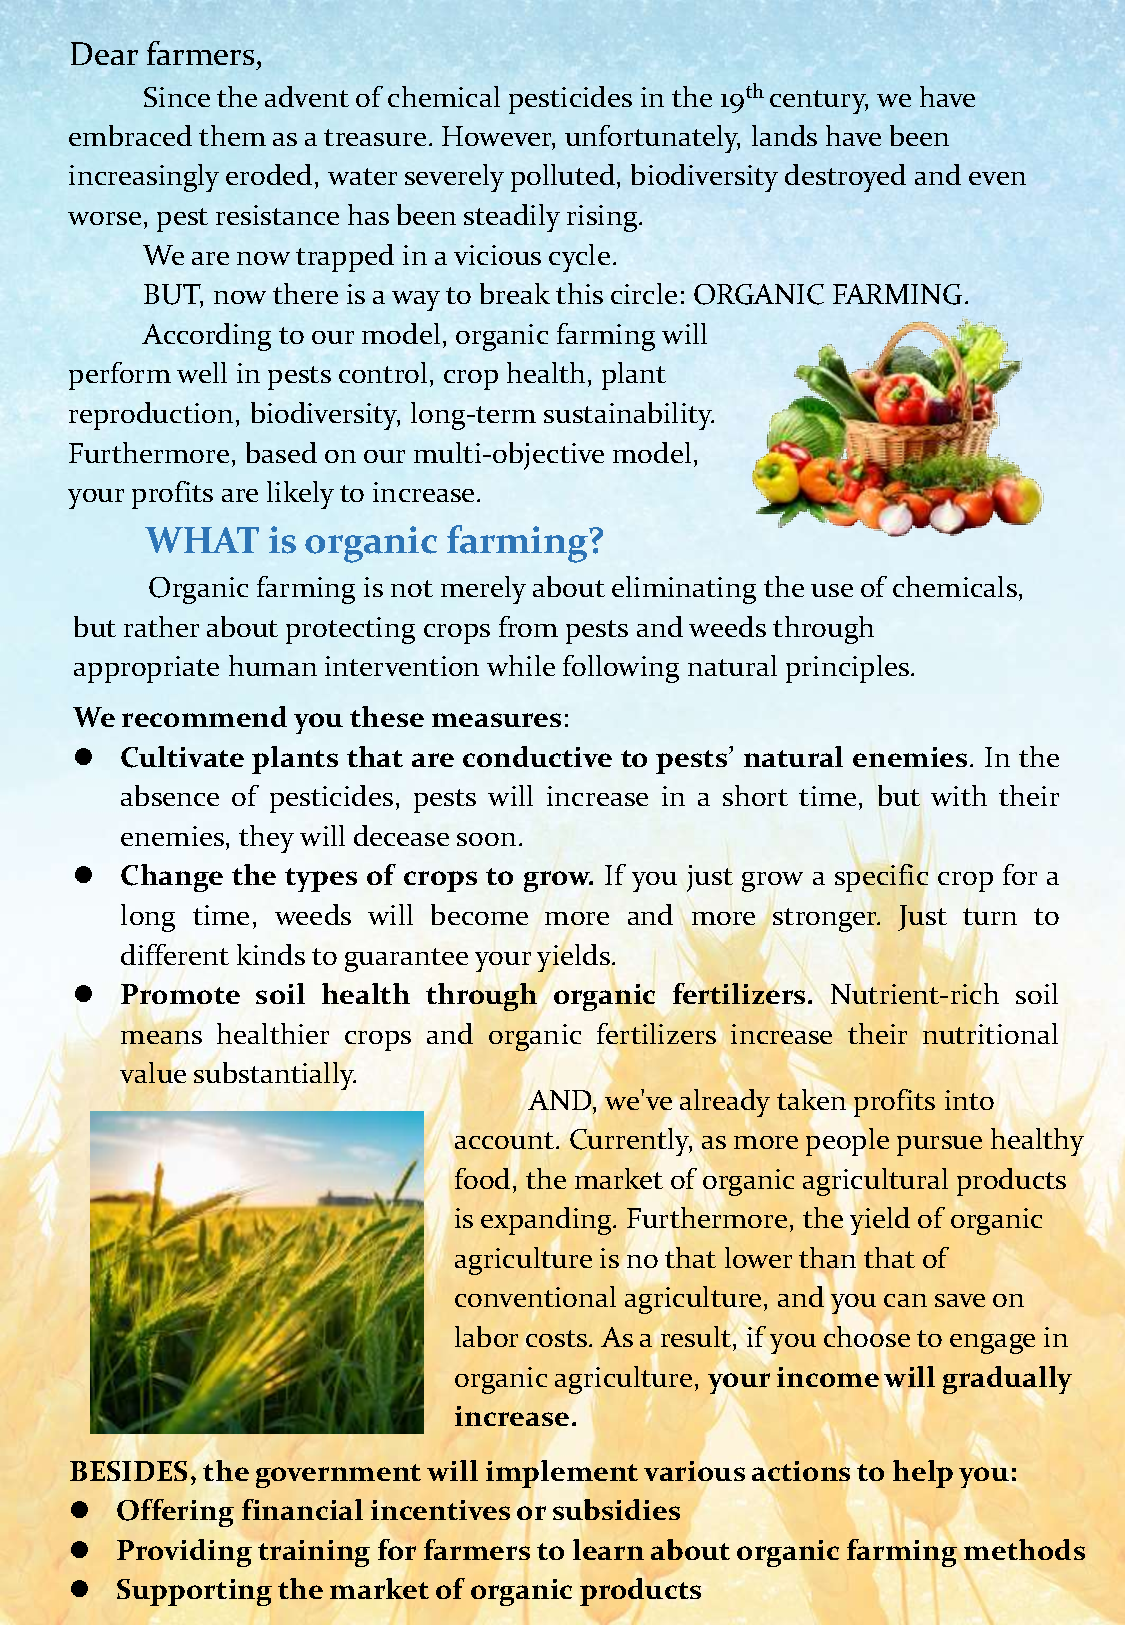
\includepdf[pages=1,scale=1,fitpaper=true]{./figures/xin.pdf}
%%%%%%%%%% 正文结束 %%%%%%%%%%%%
%%%%%%%%% 参考文献开始 %%%%%%%%%%%%
\addcontentsline{toc}{section}{References} 
\newpage
\begin{thebibliography}{00}
	
\bibitem{1} 
Craven, D.; Eisenhauer, N.; Hautier, Y.; et al. Multiple facets of biodiversity drive the diversity-stability relationship [J]. \emph{Nature ecology\& evolution}, \textbf{2018}, \emph{2}, 1579--1587.
		
\bibitem{2}
Mougi, A. Ecosystem engineering and food web stability [J]. \emph{Scientific reports}, \textbf{2024}, \emph{14}, DOI: 10.1038/s41598-024-70626-w 
		
		
\bibitem{3} 
Hatton, I.A.; Mazzarisi, O.; Altieri, A.; Smerlak, M. Diversity begets stability: Sublinear growth and competitive coexistence across ecosystems [J]. \emph{Science}, \textbf{2024}, \emph{383}, DOI:10.1126/science.adg8488


\bibitem{4}
Zhao, J.; Yu, L; Newbold, T.; etc. Biodiversity responses to agricultural practices in cropland and natural habitats [J]. \emph{Science of the Total Environment}, \textbf{2024}, \emph{922}, DOI:10.1016/j.scitotenv.2024.171296

\bibitem{5}
\textbf{URL: }\textit{https://ourworldindata.org}

\bibitem{6}
Yang T.;Sun Y. Evaluation of the net value of paddy ecosystem services in China[J]. \emph{China Agric. Univ},  \textbf{2020},  \emph{25}, 159-172.

\bibitem{7}
Xu, GH.;Yang, JJ; Research progress on stability mechanisms of food webs; a hierarchy-based framework[J].\emph{Acta Ecologica Sinica}, \textbf{2022}, \emph{42(20)}, 8493-8494 

\bibitem{8}
Seufert,V.;Ramankutty,N.Many shades of gray—The context-dependent performance of organic agriculture[J]. \emph{Science Adcances}, \textbf{2017},\emph{3}, DOI:10.1126/sciadv.1602638

\bibitem{9}
Muneret, L.; Mitchell, M.;Seufert, V.;et al.Evidence that organic farming promotes pest control[J].\emph{Nature sustainability},\textbf{2018},\emph{1},361–368.

\bibitem{10}
Tuck,S.; Winqvist,C.;Mota F.;et al. Land-use intensity and the effects of organic farming on biodiversity: a hierarchical meta-analysis[J].\emph{Journal of Applied Ecology},\textbf{2014},\emph{51},746–755.



\end{thebibliography}
%%%%%%%%% 参考文献结束 %%%%%%%%%


% AI 使用报告
\newpage
\begin{center}
    \textbf{\Large{AI Use Report}}
\end{center}

\addcontentsline{toc}{section}{AI Use Report}  
1. OpenAI ChatGPT(Jan 24, 2025 version, ChatGPT-4)\\
\hspace{2em}\textbf{Query}: When the forest is converted for agricultural use, what species would be in that ecosystem?

\textbf{Output}: When forests are converted into farmland, the ecosystem typically undergoes significant changes, affecting the species composition. The plant, animal, and microbial populations of the original forest ecosystem may decrease or disappear, while new species may gradually enter. Common changes in populations include:

Plant Populations: Native forest plants, such as trees and shrubs, are usually replaced by crops. Initially, the farmland may contain some weeds, herbaceous plants, and agricultural crops (such as corn, wheat, rice, etc.). Over time, drought-tolerant or nutrient-poor soil-tolerant plants may become dominant.

Insect Populations: Forest insects, such as tree pests and forest-dwelling insects, may decrease or be replaced. Farmland may host agricultural pests, pollinating insects (like bees), and other insects adapted to the agricultural environment (such as aphids, flea beetles, etc.).

Microbial Populations: Forest soils, rich in organic material, provide a favorable environment for microorganisms, but the transition to farmland may change the nutrient levels and soil structure, altering the microbial populations. Farmland microbial populations typically include pesticide-resistant microorganisms, some rhizosphere microorganisms, and soil bacteria that help decompose organic matter.

Animal Populations: Animal populations from the forest, particularly species reliant on trees for habitat (such as birds and mammals), may decrease or migrate. Farmland may see an increase in species that feed on crops, such as small rodents and birds.

Natural Enemies and Predators: With the emergence of farmland, the populations of natural enemies (such as certain birds, mammals) and predatory insects may also change. For example, farmland may see the introduction of natural pest controllers like spiders and parasitic wasps.

These changes in populations typically affect ecological balance and biodiversity, with farming practices (such as pesticide use, fertilization, irrigation, etc.) having a significant impact on the survival and migration of species.

\textbf{Explanation}: Our team are not sure about the original species of the newly-converted forest, so we inquired ChatGPT to get some inspiration.

2. OpenAI ChatGPT(Jan 26, 2025 version, ChatGPT-4)\\
\hspace{2em}\textbf{Query}: What does Cellular Automaton mean?

\textbf{Output}: A Cellular Automaton (CA) is a discrete mathematical model used to simulate complex systems and processes. It consists of a set of rules, and each unit (called a cell) can have different states. Cells interact with each other and change their states based on specific rules. Cellular automata are widely applied in fields such as computer science, physics, and biology, especially for simulating self-organizing phenomena, complex systems, and ecological models.

Key features of cellular automata include:

Grid Structure: Cellular automata typically exist in a regular grid format, where each grid cell is called a cell. The cells can be in two dimensions, three dimensions, or higher dimensions.

State: Each cell has a state, often represented by discrete values (e.g., 0 or 1, indicating dead or alive). These states are updated based on the states of neighboring cells according to a set of rules.

Neighborhood: Cells have a neighborhood relationship with surrounding cells. Common neighborhoods include Moore neighborhood (8 neighbors) and Von Neumann neighborhood (4 neighbors).

Update Rules: A cell's state is updated according to a set of rules, which are based on the states of the neighboring cells. These rules can be simple or complex, and they determine the system's behavior and evolution.

Discreteness: Both time and space are discrete, with the cell states being updated at each time step.

A classic example of a cellular automaton is Conway's Game of Life, which simulates the life and death of organisms based on simple rules, demonstrating complex life phenomena.

Cellular automata have broad applications, including image processing, fluid dynamics, ecological models, and neural networks.

\textbf{Explanation}:While reading a literature on species competition, we came across the concept of cellular automata, where a cell influence and is influenced by its eight neighbors. This led us to realise that convolution can be used to model the impact of one species on another.

%%%%%%%%% 全文结束 %%%%%%%%%%%%%
\end{document}
\end
